\documentclass[twoside]{book}

% Packages required by doxygen
\usepackage{fixltx2e}
\usepackage{calc}
\usepackage{doxygen}
\usepackage{graphicx}
\usepackage[utf8]{inputenc}
\usepackage{makeidx}
\usepackage{multicol}
\usepackage{multirow}
\PassOptionsToPackage{warn}{textcomp}
\usepackage{textcomp}
\usepackage[nointegrals]{wasysym}
\usepackage[table]{xcolor}

% NLS support packages
\usepackage[brazil]{babel}
% Font selection
\usepackage[T1]{fontenc}
\usepackage{mathptmx}
\usepackage[scaled=.90]{helvet}
\usepackage{courier}
\usepackage{amssymb}
\usepackage{sectsty}
\renewcommand{\familydefault}{\sfdefault}
\allsectionsfont{%
  \fontseries{bc}\selectfont%
  \color{darkgray}%
}
\renewcommand{\DoxyLabelFont}{%
  \fontseries{bc}\selectfont%
  \color{darkgray}%
}
\newcommand{\+}{\discretionary{\mbox{\scriptsize$\hookleftarrow$}}{}{}}

% Page & text layout
\usepackage{geometry}
\geometry{%
  a4paper,%
  top=2.5cm,%
  bottom=2.5cm,%
  left=2.5cm,%
  right=2.5cm%
}
\tolerance=750
\hfuzz=15pt
\hbadness=750
\setlength{\emergencystretch}{15pt}
\setlength{\parindent}{0cm}
\setlength{\parskip}{0.2cm}
\makeatletter
\renewcommand{\paragraph}{%
  \@startsection{paragraph}{4}{0ex}{-1.0ex}{1.0ex}{%
    \normalfont\normalsize\bfseries\SS@parafont%
  }%
}
\renewcommand{\subparagraph}{%
  \@startsection{subparagraph}{5}{0ex}{-1.0ex}{1.0ex}{%
    \normalfont\normalsize\bfseries\SS@subparafont%
  }%
}
\makeatother

% Headers & footers
\usepackage{fancyhdr}
\pagestyle{fancyplain}
\fancyhead[LE]{\fancyplain{}{\bfseries\thepage}}
\fancyhead[CE]{\fancyplain{}{}}
\fancyhead[RE]{\fancyplain{}{\bfseries\leftmark}}
\fancyhead[LO]{\fancyplain{}{\bfseries\rightmark}}
\fancyhead[CO]{\fancyplain{}{}}
\fancyhead[RO]{\fancyplain{}{\bfseries\thepage}}
\fancyfoot[LE]{\fancyplain{}{}}
\fancyfoot[CE]{\fancyplain{}{}}
\fancyfoot[RE]{\fancyplain{}{\bfseries\scriptsize Gerado em Sexta, 20 de Junho de 2014 00\+:07\+:31 para Spartacus por Doxygen }}
\fancyfoot[LO]{\fancyplain{}{\bfseries\scriptsize Gerado em Sexta, 20 de Junho de 2014 00\+:07\+:31 para Spartacus por Doxygen }}
\fancyfoot[CO]{\fancyplain{}{}}
\fancyfoot[RO]{\fancyplain{}{}}
\renewcommand{\footrulewidth}{0.4pt}
\renewcommand{\chaptermark}[1]{%
  \markboth{#1}{}%
}
\renewcommand{\sectionmark}[1]{%
  \markright{\thesection\ #1}%
}

% Indices & bibliography
\usepackage{natbib}
\usepackage[titles]{tocloft}
\setcounter{tocdepth}{3}
\setcounter{secnumdepth}{5}
\makeindex

% Hyperlinks (required, but should be loaded last)
\usepackage{ifpdf}
\ifpdf
  \usepackage[pdftex,pagebackref=true]{hyperref}
\else
  \usepackage[ps2pdf,pagebackref=true]{hyperref}
\fi
\hypersetup{%
  colorlinks=true,%
  linkcolor=blue,%
  citecolor=blue,%
  unicode%
}

% Custom commands
\newcommand{\clearemptydoublepage}{%
  \newpage{\pagestyle{empty}\cleardoublepage}%
}


%===== C O N T E N T S =====

\begin{document}

% Titlepage & ToC
\hypersetup{pageanchor=false,
             bookmarks=true,
             bookmarksnumbered=true,
             pdfencoding=unicode
            }
\pagenumbering{roman}
\begin{titlepage}
\vspace*{7cm}
\begin{center}%
{\Large Spartacus \\[1ex]\large 0.\+17.\+1 }\\
\vspace*{1cm}
{\large Gerado por Doxygen 1.8.7}\\
\vspace*{0.5cm}
{\small Sexta, 20 de Junho de 2014 00:07:31}\\
\end{center}
\end{titlepage}
\clearemptydoublepage
\tableofcontents
\clearemptydoublepage
\pagenumbering{arabic}
\hypersetup{pageanchor=true}

%--- Begin generated contents ---
\chapter{Namespaces}
\section{Lista de Namespaces}
Esta é a lista de todos os Namespaces documentados com suas respectivas descrições\+:\begin{DoxyCompactList}
\item\contentsline{section}{\hyperlink{namespaceSpartacus}{Spartacus} }{\pageref{namespaceSpartacus}}{}
\item\contentsline{section}{\hyperlink{namespaceSpartacus_1_1Database}{Spartacus.\+Database} }{\pageref{namespaceSpartacus_1_1Database}}{}
\item\contentsline{section}{\hyperlink{namespaceSpartacus_1_1Reporting}{Spartacus.\+Reporting} }{\pageref{namespaceSpartacus_1_1Reporting}}{}
\item\contentsline{section}{\hyperlink{namespaceSpartacus_1_1Utils}{Spartacus.\+Utils} }{\pageref{namespaceSpartacus_1_1Utils}}{}
\end{DoxyCompactList}

\chapter{Índice Hierárquico}
\section{Hierarquia de Classes}
Esta lista de hierarquias está parcialmente ordenada (ordem alfabética)\+:\begin{DoxyCompactList}
\item \contentsline{section}{Spartacus.\+Database.\+Command}{\pageref{classSpartacus_1_1Database_1_1Command}}{}
\item \contentsline{section}{Spartacus.\+Utils.\+Exception}{\pageref{classSpartacus_1_1Utils_1_1Exception}}{}
\item \contentsline{section}{Spartacus.\+Database.\+Exception}{\pageref{classSpartacus_1_1Database_1_1Exception}}{}
\item \contentsline{section}{Spartacus.\+Reporting.\+Exception}{\pageref{classSpartacus_1_1Reporting_1_1Exception}}{}
\item \contentsline{section}{Spartacus.\+Utils.\+File}{\pageref{classSpartacus_1_1Utils_1_1File}}{}
\item \contentsline{section}{Spartacus.\+Utils.\+File\+Explorer}{\pageref{classSpartacus_1_1Utils_1_1FileExplorer}}{}
\item \contentsline{section}{Spartacus.\+Database.\+Generic}{\pageref{classSpartacus_1_1Database_1_1Generic}}{}
\begin{DoxyCompactList}
\item \contentsline{section}{Spartacus.\+Database.\+Firebird}{\pageref{classSpartacus_1_1Database_1_1Firebird}}{}
\item \contentsline{section}{Spartacus.\+Database.\+Mysql}{\pageref{classSpartacus_1_1Database_1_1Mysql}}{}
\item \contentsline{section}{Spartacus.\+Database.\+Odbc}{\pageref{classSpartacus_1_1Database_1_1Odbc}}{}
\item \contentsline{section}{Spartacus.\+Database.\+Oledb}{\pageref{classSpartacus_1_1Database_1_1Oledb}}{}
\item \contentsline{section}{Spartacus.\+Database.\+Sqlite}{\pageref{classSpartacus_1_1Database_1_1Sqlite}}{}
\end{DoxyCompactList}
\item \contentsline{section}{Spartacus.\+Database.\+Parameter}{\pageref{classSpartacus_1_1Database_1_1Parameter}}{}
\item \contentsline{section}{Spartacus.\+Utils.\+Synchronizer}{\pageref{classSpartacus_1_1Utils_1_1Synchronizer}}{}
\end{DoxyCompactList}

\chapter{Índice das Estruturas de Dados}
\section{Estruturas de Dados}
Aqui estão as estruturas de dados, uniões e suas respectivas descrições\+:\begin{DoxyCompactList}
\item\contentsline{section}{\hyperlink{classSpartacus_1_1Reporting_1_1Block}{Spartacus.\+Reporting.\+Block} \\*Classe \hyperlink{classSpartacus_1_1Reporting_1_1Block}{Block}. Representa um bloco que pode conter qualquer informação. O cabeçalho do relatório e o rodapé do relatório são blocos. }{\pageref{classSpartacus_1_1Reporting_1_1Block}}{}
\item\contentsline{section}{\hyperlink{classSpartacus_1_1Reporting_1_1Border}{Spartacus.\+Reporting.\+Border} \\*Classe \hyperlink{classSpartacus_1_1Reporting_1_1Border}{Border}. Armazena informações sobre quais bordas devem ser ativadas. }{\pageref{classSpartacus_1_1Reporting_1_1Border}}{}
\item\contentsline{section}{\hyperlink{classSpartacus_1_1Net_1_1Client}{Spartacus.\+Net.\+Client} \\*Classe \hyperlink{classSpartacus_1_1Net_1_1Client}{Client}. Herda da classe \hyperlink{classSpartacus_1_1Net_1_1Endpoint}{Spartacus.\+Net.\+Endpoint}. }{\pageref{classSpartacus_1_1Net_1_1Client}}{}
\item\contentsline{section}{\hyperlink{classSpartacus_1_1Database_1_1Command}{Spartacus.\+Database.\+Command} \\*Classe \hyperlink{classSpartacus_1_1Database_1_1Command}{Command}. Representa um comando S\+Q\+L que pode possuir parâmetros entre \#. }{\pageref{classSpartacus_1_1Database_1_1Command}}{}
\item\contentsline{section}{\hyperlink{classSpartacus_1_1Net_1_1Cryptor}{Spartacus.\+Net.\+Cryptor} \\*Classe \hyperlink{classSpartacus_1_1Net_1_1Cryptor}{Cryptor}. Objeto genérico que pode criptografar e descriptografar strings e arquivos. }{\pageref{classSpartacus_1_1Net_1_1Cryptor}}{}
\item\contentsline{section}{\hyperlink{classSpartacus_1_1Net_1_1Endpoint}{Spartacus.\+Net.\+Endpoint} \\*Classe \hyperlink{classSpartacus_1_1Net_1_1Endpoint}{Endpoint}. Representa um ponto de comunicação, que pode ser tanto um cliente ou um servidor. }{\pageref{classSpartacus_1_1Net_1_1Endpoint}}{}
\item\contentsline{section}{\hyperlink{classSpartacus_1_1Utils_1_1Exception}{Spartacus.\+Utils.\+Exception} \\*Classe \hyperlink{classSpartacus_1_1Utils_1_1Exception}{Spartacus.\+Utils.\+Exception}. Herda da classe System.\+Exception. }{\pageref{classSpartacus_1_1Utils_1_1Exception}}{}
\item\contentsline{section}{\hyperlink{classSpartacus_1_1Net_1_1Exception}{Spartacus.\+Net.\+Exception} \\*Classe \hyperlink{classSpartacus_1_1Net_1_1Exception}{Spartacus.\+Net.\+Exception}. Herda da classe System.\+Exception. }{\pageref{classSpartacus_1_1Net_1_1Exception}}{}
\item\contentsline{section}{\hyperlink{classSpartacus_1_1Database_1_1Exception}{Spartacus.\+Database.\+Exception} \\*Classe \hyperlink{classSpartacus_1_1Database_1_1Exception}{Spartacus.\+Database.\+Exception}. Herda da classe System.\+Exception. }{\pageref{classSpartacus_1_1Database_1_1Exception}}{}
\item\contentsline{section}{\hyperlink{classSpartacus_1_1Reporting_1_1Exception}{Spartacus.\+Reporting.\+Exception} \\*Classe \hyperlink{classSpartacus_1_1Reporting_1_1Exception}{Spartacus.\+Reporting.\+Exception}. Herda da classe System.\+Exception. }{\pageref{classSpartacus_1_1Reporting_1_1Exception}}{}
\item\contentsline{section}{\hyperlink{classSpartacus_1_1Reporting_1_1Field}{Spartacus.\+Reporting.\+Field} \\*Classe \hyperlink{classSpartacus_1_1Reporting_1_1Field}{Field}. Representa um campo de dados do relatório. }{\pageref{classSpartacus_1_1Reporting_1_1Field}}{}
\item\contentsline{section}{\hyperlink{classSpartacus_1_1Utils_1_1File}{Spartacus.\+Utils.\+File} \\*Classe \hyperlink{classSpartacus_1_1Utils_1_1File}{File}. Representa um arquivo ou um diretório. Pode ser usado em listas de arquivos para processamento em massa, ou para construção de árvores de arquivos. }{\pageref{classSpartacus_1_1Utils_1_1File}}{}
\item\contentsline{section}{\hyperlink{classSpartacus_1_1Utils_1_1FileExplorer}{Spartacus.\+Utils.\+File\+Explorer} \\*Classe \hyperlink{classSpartacus_1_1Utils_1_1FileExplorer}{File\+Explorer}. Representa um explorador de arquivos genérico, que pode ser usado em qualquer interface (prompt de comando, desktop ou web). }{\pageref{classSpartacus_1_1Utils_1_1FileExplorer}}{}
\item\contentsline{section}{\hyperlink{classSpartacus_1_1Database_1_1Firebird}{Spartacus.\+Database.\+Firebird} \\*Classe \hyperlink{classSpartacus_1_1Database_1_1Firebird}{Spartacus.\+Database.\+Firebird}. Herda da classe \hyperlink{classSpartacus_1_1Database_1_1Generic}{Spartacus.\+Database.\+Generic}. Utiliza o \hyperlink{classSpartacus_1_1Database_1_1Firebird}{Firebird} .N\+E\+T Provider para acessar um S\+G\+B\+D \hyperlink{classSpartacus_1_1Database_1_1Firebird}{Firebird}. }{\pageref{classSpartacus_1_1Database_1_1Firebird}}{}
\item\contentsline{section}{\hyperlink{classSpartacus_1_1Reporting_1_1Font}{Spartacus.\+Reporting.\+Font} \\*Classe Fonte. }{\pageref{classSpartacus_1_1Reporting_1_1Font}}{}
\item\contentsline{section}{\hyperlink{classSpartacus_1_1Database_1_1Generic}{Spartacus.\+Database.\+Generic} \\*Classe abstrata \hyperlink{classSpartacus_1_1Database_1_1Generic}{Spartacus.\+Database.\+Generic}. Armazena informações de conexão que são genéricas a qualquer S\+G\+B\+D. Provê polimorfismo, por ser uma classe abstrata. }{\pageref{classSpartacus_1_1Database_1_1Generic}}{}
\item\contentsline{section}{\hyperlink{classSpartacus_1_1Reporting_1_1Group}{Spartacus.\+Reporting.\+Group} \\*Classe \hyperlink{classSpartacus_1_1Reporting_1_1Group}{Group}. Representa um agrupamento de dados do relatório. }{\pageref{classSpartacus_1_1Reporting_1_1Group}}{}
\item\contentsline{section}{\hyperlink{classSpartacus_1_1Database_1_1Mysql}{Spartacus.\+Database.\+Mysql} \\*Classe \hyperlink{classSpartacus_1_1Database_1_1Mysql}{Spartacus.\+Database.\+Mysql}. Herda da classe \hyperlink{classSpartacus_1_1Database_1_1Generic}{Spartacus.\+Database.\+Generic}. Utiliza o My\+S\+Q\+L .N\+E\+T Provider para acessar um S\+G\+B\+D My\+S\+Q\+L. }{\pageref{classSpartacus_1_1Database_1_1Mysql}}{}
\item\contentsline{section}{\hyperlink{classSpartacus_1_1Reporting_1_1Object}{Spartacus.\+Reporting.\+Object} \\*Classe \hyperlink{classSpartacus_1_1Reporting_1_1Object}{Object}. Representa um objeto que pode ser renderizado dentro de um \hyperlink{classSpartacus_1_1Reporting_1_1Block}{Spartacus.\+Reporting.\+Block}. }{\pageref{classSpartacus_1_1Reporting_1_1Object}}{}
\item\contentsline{section}{\hyperlink{classSpartacus_1_1Database_1_1Odbc}{Spartacus.\+Database.\+Odbc} \\*Classe \hyperlink{classSpartacus_1_1Database_1_1Odbc}{Spartacus.\+Database.\+Odbc}. Herda da classe \hyperlink{classSpartacus_1_1Database_1_1Generic}{Spartacus.\+Database.\+Generic}. Utiliza a implementação O\+D\+B\+C (Open \hyperlink{namespaceSpartacus_1_1Database}{Database} Connectivity) para acessar qualquer S\+G\+B\+D. }{\pageref{classSpartacus_1_1Database_1_1Odbc}}{}
\item\contentsline{section}{\hyperlink{classSpartacus_1_1Database_1_1Oledb}{Spartacus.\+Database.\+Oledb} \\*Classe \hyperlink{classSpartacus_1_1Database_1_1Oledb}{Spartacus.\+Database.\+Oledb}; Herda da classe \hyperlink{classSpartacus_1_1Database_1_1Generic}{Spartacus.\+Database.\+Generic}. Utiliza a implementação O\+L\+E D\+B para acessar qualquer S\+G\+B\+D. }{\pageref{classSpartacus_1_1Database_1_1Oledb}}{}
\item\contentsline{section}{\hyperlink{classSpartacus_1_1Database_1_1Parameter}{Spartacus.\+Database.\+Parameter} \\*Classe \hyperlink{classSpartacus_1_1Database_1_1Parameter}{Parameter}. Representa um parâmetro da classe \hyperlink{classSpartacus_1_1Database_1_1Command}{Spartacus.\+Database.\+Command}. }{\pageref{classSpartacus_1_1Database_1_1Parameter}}{}
\item\contentsline{section}{\hyperlink{classSpartacus_1_1Database_1_1Postgresql}{Spartacus.\+Database.\+Postgresql} \\*Classe \hyperlink{classSpartacus_1_1Database_1_1Postgresql}{Spartacus.\+Database.\+Postgresql}. Herda da classe \hyperlink{classSpartacus_1_1Database_1_1Generic}{Spartacus.\+Database.\+Generic}. Utiliza o Npgsql .N\+E\+T Provider para acessar um S\+G\+B\+D Postgre\+S\+Q\+L. }{\pageref{classSpartacus_1_1Database_1_1Postgresql}}{}
\item\contentsline{section}{\hyperlink{classSpartacus_1_1Reporting_1_1Report}{Spartacus.\+Reporting.\+Report} \\*Classe \hyperlink{classSpartacus_1_1Reporting_1_1Report}{Report}. Representa um relatório em P\+D\+F. }{\pageref{classSpartacus_1_1Reporting_1_1Report}}{}
\item\contentsline{section}{\hyperlink{classSpartacus_1_1Reporting_1_1Settings}{Spartacus.\+Reporting.\+Settings} \\*Classe \hyperlink{classSpartacus_1_1Reporting_1_1Settings}{Settings}. Armazena informações gerais sobre o relatório. }{\pageref{classSpartacus_1_1Reporting_1_1Settings}}{}
\item\contentsline{section}{\hyperlink{classSpartacus_1_1Database_1_1Sqlite}{Spartacus.\+Database.\+Sqlite} \\*Classe \hyperlink{classSpartacus_1_1Database_1_1Sqlite}{Spartacus.\+Database.\+Sqlite}. Herda da classe \hyperlink{classSpartacus_1_1Database_1_1Generic}{Spartacus.\+Database.\+Generic}. Utiliza o Mono.\+Data.\+Sqlite para acessar um S\+G\+B\+D \hyperlink{classSpartacus_1_1Database_1_1Sqlite}{Sqlite}. }{\pageref{classSpartacus_1_1Database_1_1Sqlite}}{}
\item\contentsline{section}{\hyperlink{classSpartacus_1_1Utils_1_1Synchronizer}{Spartacus.\+Utils.\+Synchronizer} \\*Classe \hyperlink{classSpartacus_1_1Utils_1_1Synchronizer}{Synchronizer}. Sincroniza duas pastas. }{\pageref{classSpartacus_1_1Utils_1_1Synchronizer}}{}
\end{DoxyCompactList}

\chapter{Namespaces}
\hypertarget{namespaceSpartacus}{\section{Pacote Spartacus}
\label{namespaceSpartacus}\index{Spartacus@{Spartacus}}
}
\subsection*{Namespaces}
\begin{DoxyCompactItemize}
\item 
package \hyperlink{namespaceSpartacus_1_1Database}{Database}
\item 
package \hyperlink{namespaceSpartacus_1_1Forms}{Forms}
\item 
package \hyperlink{namespaceSpartacus_1_1Net}{Net}
\item 
package \hyperlink{namespaceSpartacus_1_1Reporting}{Reporting}
\item 
package \hyperlink{namespaceSpartacus_1_1Utils}{Utils}
\end{DoxyCompactItemize}

\hypertarget{namespaceSpartacus_1_1Database}{\section{Pacote Spartacus.\+Database}
\label{namespaceSpartacus_1_1Database}\index{Spartacus.\+Database@{Spartacus.\+Database}}
}
\subsection*{Estruturas de Dados}
\begin{DoxyCompactItemize}
\item 
class \hyperlink{classSpartacus_1_1Database_1_1Command}{Command}
\begin{DoxyCompactList}\small\item\em Classe \hyperlink{classSpartacus_1_1Database_1_1Command}{Command}. Representa um comando S\+Q\+L que pode possuir parâmetros entre \#. \end{DoxyCompactList}\item 
class \hyperlink{classSpartacus_1_1Database_1_1Exception}{Exception}
\begin{DoxyCompactList}\small\item\em Classe \hyperlink{classSpartacus_1_1Database_1_1Exception}{Spartacus.\+Database.\+Exception}. Herda da classe System.\+Exception. \end{DoxyCompactList}\item 
class \hyperlink{classSpartacus_1_1Database_1_1Firebird}{Firebird}
\begin{DoxyCompactList}\small\item\em Classe \hyperlink{classSpartacus_1_1Database_1_1Firebird}{Spartacus.\+Database.\+Firebird}. Herda da classe \hyperlink{classSpartacus_1_1Database_1_1Generic}{Spartacus.\+Database.\+Generic}. Utiliza o \hyperlink{classSpartacus_1_1Database_1_1Firebird}{Firebird} .N\+E\+T Provider para acessar um S\+G\+B\+D \hyperlink{classSpartacus_1_1Database_1_1Firebird}{Firebird}. \end{DoxyCompactList}\item 
class \hyperlink{classSpartacus_1_1Database_1_1Generic}{Generic}
\begin{DoxyCompactList}\small\item\em Classe abstrata \hyperlink{classSpartacus_1_1Database_1_1Generic}{Spartacus.\+Database.\+Generic}. Armazena informações de conexão que são genéricas a qualquer S\+G\+B\+D. Provê polimorfismo, por ser uma classe abstrata. \end{DoxyCompactList}\item 
class \hyperlink{classSpartacus_1_1Database_1_1Mysql}{Mysql}
\begin{DoxyCompactList}\small\item\em Classe \hyperlink{classSpartacus_1_1Database_1_1Mysql}{Spartacus.\+Database.\+Mysql}. Herda da classe \hyperlink{classSpartacus_1_1Database_1_1Generic}{Spartacus.\+Database.\+Generic}. Utiliza o My\+S\+Q\+L .N\+E\+T Provider para acessar um S\+G\+B\+D My\+S\+Q\+L. \end{DoxyCompactList}\item 
class \hyperlink{classSpartacus_1_1Database_1_1Odbc}{Odbc}
\begin{DoxyCompactList}\small\item\em Classe \hyperlink{classSpartacus_1_1Database_1_1Odbc}{Spartacus.\+Database.\+Odbc}. Herda da classe \hyperlink{classSpartacus_1_1Database_1_1Generic}{Spartacus.\+Database.\+Generic}. Utiliza a implementação O\+D\+B\+C (Open \hyperlink{namespaceSpartacus_1_1Database}{Database} Connectivity) para acessar qualquer S\+G\+B\+D. \end{DoxyCompactList}\item 
class \hyperlink{classSpartacus_1_1Database_1_1Oledb}{Oledb}
\begin{DoxyCompactList}\small\item\em Classe \hyperlink{classSpartacus_1_1Database_1_1Oledb}{Spartacus.\+Database.\+Oledb}; Herda da classe \hyperlink{classSpartacus_1_1Database_1_1Generic}{Spartacus.\+Database.\+Generic}. Utiliza a implementação O\+L\+E D\+B para acessar qualquer S\+G\+B\+D. \end{DoxyCompactList}\item 
class \hyperlink{classSpartacus_1_1Database_1_1Parameter}{Parameter}
\begin{DoxyCompactList}\small\item\em Classe \hyperlink{classSpartacus_1_1Database_1_1Parameter}{Parameter}. Representa um parâmetro da classe \hyperlink{classSpartacus_1_1Database_1_1Command}{Spartacus.\+Database.\+Command}. \end{DoxyCompactList}\item 
class \hyperlink{classSpartacus_1_1Database_1_1Postgresql}{Postgresql}
\begin{DoxyCompactList}\small\item\em Classe \hyperlink{classSpartacus_1_1Database_1_1Postgresql}{Spartacus.\+Database.\+Postgresql}. Herda da classe \hyperlink{classSpartacus_1_1Database_1_1Generic}{Spartacus.\+Database.\+Generic}. Utiliza o Npgsql .N\+E\+T Provider para acessar um S\+G\+B\+D Postgre\+S\+Q\+L. \end{DoxyCompactList}\item 
class \hyperlink{classSpartacus_1_1Database_1_1Sqlite}{Sqlite}
\begin{DoxyCompactList}\small\item\em Classe \hyperlink{classSpartacus_1_1Database_1_1Sqlite}{Spartacus.\+Database.\+Sqlite}. Herda da classe \hyperlink{classSpartacus_1_1Database_1_1Generic}{Spartacus.\+Database.\+Generic}. Utiliza o Mono.\+Data.\+Sqlite para acessar um S\+G\+B\+D \hyperlink{classSpartacus_1_1Database_1_1Sqlite}{Sqlite}. \end{DoxyCompactList}\end{DoxyCompactItemize}
\subsection*{Enumerações}
\begin{DoxyCompactItemize}
\item 
enum \hyperlink{namespaceSpartacus_1_1Database_a9d4c2be7c9bc257b8d34c84b43e5ec32}{Type} 
\begin{DoxyCompactList}\small\item\em Tipos de Dados. \end{DoxyCompactList}\item 
enum \hyperlink{namespaceSpartacus_1_1Database_a5c77dce887cad55e7ea67f0f98a7d71f}{Locale} 
\begin{DoxyCompactList}\small\item\em Representações de números reais\+: A\+M\+E\+R\+I\+C\+A\+N\+: separador decimal\+: . separador de milhar\+: , E\+U\+R\+O\+P\+E\+A\+N\+: separador decimal\+: , separador de milhar\+: . \end{DoxyCompactList}\end{DoxyCompactItemize}


\subsection{Enumerações}
\hypertarget{namespaceSpartacus_1_1Database_a5c77dce887cad55e7ea67f0f98a7d71f}{\index{Spartacus\+::\+Database@{Spartacus\+::\+Database}!Locale@{Locale}}
\index{Locale@{Locale}!Spartacus\+::\+Database@{Spartacus\+::\+Database}}
\subsubsection[{Locale}]{\setlength{\rightskip}{0pt plus 5cm}enum {\bf Spartacus.\+Database.\+Locale}}}\label{namespaceSpartacus_1_1Database_a5c77dce887cad55e7ea67f0f98a7d71f}


Representações de números reais\+: A\+M\+E\+R\+I\+C\+A\+N\+: separador decimal\+: . separador de milhar\+: , E\+U\+R\+O\+P\+E\+A\+N\+: separador decimal\+: , separador de milhar\+: . 

\hypertarget{namespaceSpartacus_1_1Database_a9d4c2be7c9bc257b8d34c84b43e5ec32}{\index{Spartacus\+::\+Database@{Spartacus\+::\+Database}!Type@{Type}}
\index{Type@{Type}!Spartacus\+::\+Database@{Spartacus\+::\+Database}}
\subsubsection[{Type}]{\setlength{\rightskip}{0pt plus 5cm}enum {\bf Spartacus.\+Database.\+Type}}}\label{namespaceSpartacus_1_1Database_a9d4c2be7c9bc257b8d34c84b43e5ec32}


Tipos de Dados. 


\hypertarget{namespaceSpartacus_1_1Reporting}{\section{Pacote Spartacus.\+Reporting}
\label{namespaceSpartacus_1_1Reporting}\index{Spartacus.\+Reporting@{Spartacus.\+Reporting}}
}
\subsection*{Estruturas de Dados}
\begin{DoxyCompactItemize}
\item 
class \hyperlink{classSpartacus_1_1Reporting_1_1Block}{Block}
\begin{DoxyCompactList}\small\item\em Classe \hyperlink{classSpartacus_1_1Reporting_1_1Block}{Block}. Representa um bloco que pode conter qualquer informação. O cabeçalho do relatório e o rodapé do relatório são blocos. \end{DoxyCompactList}\item 
class \hyperlink{classSpartacus_1_1Reporting_1_1Border}{Border}
\begin{DoxyCompactList}\small\item\em Classe \hyperlink{classSpartacus_1_1Reporting_1_1Border}{Border}. Armazena informações sobre quais bordas devem ser ativadas. \end{DoxyCompactList}\item 
class \hyperlink{classSpartacus_1_1Reporting_1_1Exception}{Exception}
\begin{DoxyCompactList}\small\item\em Classe \hyperlink{classSpartacus_1_1Reporting_1_1Exception}{Spartacus.\+Reporting.\+Exception}. Herda da classe System.\+Exception. \end{DoxyCompactList}\item 
class \hyperlink{classSpartacus_1_1Reporting_1_1Field}{Field}
\begin{DoxyCompactList}\small\item\em Classe \hyperlink{classSpartacus_1_1Reporting_1_1Field}{Field}. Representa um campo de dados do relatório. \end{DoxyCompactList}\item 
class \hyperlink{classSpartacus_1_1Reporting_1_1Font}{Font}
\begin{DoxyCompactList}\small\item\em Classe Fonte. \end{DoxyCompactList}\item 
class \hyperlink{classSpartacus_1_1Reporting_1_1Group}{Group}
\begin{DoxyCompactList}\small\item\em Classe \hyperlink{classSpartacus_1_1Reporting_1_1Group}{Group}. Representa um agrupamento de dados do relatório. \end{DoxyCompactList}\item 
class \hyperlink{classSpartacus_1_1Reporting_1_1Object}{Object}
\begin{DoxyCompactList}\small\item\em Classe \hyperlink{classSpartacus_1_1Reporting_1_1Object}{Object}. Representa um objeto que pode ser renderizado dentro de um \hyperlink{classSpartacus_1_1Reporting_1_1Block}{Spartacus.\+Reporting.\+Block}. \end{DoxyCompactList}\item 
class \hyperlink{classSpartacus_1_1Reporting_1_1Report}{Report}
\begin{DoxyCompactList}\small\item\em Classe \hyperlink{classSpartacus_1_1Reporting_1_1Report}{Report}. Representa um relatório em P\+D\+F. \end{DoxyCompactList}\item 
class \hyperlink{classSpartacus_1_1Reporting_1_1Settings}{Settings}
\begin{DoxyCompactList}\small\item\em Classe \hyperlink{classSpartacus_1_1Reporting_1_1Settings}{Settings}. Armazena informações gerais sobre o relatório. \end{DoxyCompactList}\end{DoxyCompactItemize}
\subsection*{Enumerações}
\begin{DoxyCompactItemize}
\item 
enum \hyperlink{namespaceSpartacus_1_1Reporting_a1b74021bf4e6e2fe6eac8a1aebddd05e}{Field\+Alignment} 
\begin{DoxyCompactList}\small\item\em Alinhamento do Campo. \end{DoxyCompactList}\item 
enum \hyperlink{namespaceSpartacus_1_1Reporting_a9108ed8004cb83935ed4785cc790fddf}{Font\+Family} 
\begin{DoxyCompactList}\small\item\em Família de fonte. \end{DoxyCompactList}\item 
enum \hyperlink{namespaceSpartacus_1_1Reporting_a3727122f6fe78a79014ed0180e0ac2e3}{Object\+Type} 
\begin{DoxyCompactList}\small\item\em Tipo do Objeto. \end{DoxyCompactList}\item 
enum \hyperlink{namespaceSpartacus_1_1Reporting_a5e056b0c6896c4426cb938d08c5acb34}{Page\+Layout} 
\begin{DoxyCompactList}\small\item\em Layout da Página. \end{DoxyCompactList}\item 
enum \hyperlink{namespaceSpartacus_1_1Reporting_ab924f4d0d38ee1ef2a116121e4ec44fa}{Page\+Margin} 
\begin{DoxyCompactList}\small\item\em Tipo de margem. \end{DoxyCompactList}\end{DoxyCompactItemize}


\subsection{Enumerações}
\hypertarget{namespaceSpartacus_1_1Reporting_a1b74021bf4e6e2fe6eac8a1aebddd05e}{\index{Spartacus\+::\+Reporting@{Spartacus\+::\+Reporting}!Field\+Alignment@{Field\+Alignment}}
\index{Field\+Alignment@{Field\+Alignment}!Spartacus\+::\+Reporting@{Spartacus\+::\+Reporting}}
\subsubsection[{Field\+Alignment}]{\setlength{\rightskip}{0pt plus 5cm}enum {\bf Spartacus.\+Reporting.\+Field\+Alignment}}}\label{namespaceSpartacus_1_1Reporting_a1b74021bf4e6e2fe6eac8a1aebddd05e}


Alinhamento do Campo. 

\hypertarget{namespaceSpartacus_1_1Reporting_a9108ed8004cb83935ed4785cc790fddf}{\index{Spartacus\+::\+Reporting@{Spartacus\+::\+Reporting}!Font\+Family@{Font\+Family}}
\index{Font\+Family@{Font\+Family}!Spartacus\+::\+Reporting@{Spartacus\+::\+Reporting}}
\subsubsection[{Font\+Family}]{\setlength{\rightskip}{0pt plus 5cm}enum {\bf Spartacus.\+Reporting.\+Font\+Family}}}\label{namespaceSpartacus_1_1Reporting_a9108ed8004cb83935ed4785cc790fddf}


Família de fonte. 

\hypertarget{namespaceSpartacus_1_1Reporting_a3727122f6fe78a79014ed0180e0ac2e3}{\index{Spartacus\+::\+Reporting@{Spartacus\+::\+Reporting}!Object\+Type@{Object\+Type}}
\index{Object\+Type@{Object\+Type}!Spartacus\+::\+Reporting@{Spartacus\+::\+Reporting}}
\subsubsection[{Object\+Type}]{\setlength{\rightskip}{0pt plus 5cm}enum {\bf Spartacus.\+Reporting.\+Object\+Type}}}\label{namespaceSpartacus_1_1Reporting_a3727122f6fe78a79014ed0180e0ac2e3}


Tipo do Objeto. 

\hypertarget{namespaceSpartacus_1_1Reporting_a5e056b0c6896c4426cb938d08c5acb34}{\index{Spartacus\+::\+Reporting@{Spartacus\+::\+Reporting}!Page\+Layout@{Page\+Layout}}
\index{Page\+Layout@{Page\+Layout}!Spartacus\+::\+Reporting@{Spartacus\+::\+Reporting}}
\subsubsection[{Page\+Layout}]{\setlength{\rightskip}{0pt plus 5cm}enum {\bf Spartacus.\+Reporting.\+Page\+Layout}}}\label{namespaceSpartacus_1_1Reporting_a5e056b0c6896c4426cb938d08c5acb34}


Layout da Página. 

\hypertarget{namespaceSpartacus_1_1Reporting_ab924f4d0d38ee1ef2a116121e4ec44fa}{\index{Spartacus\+::\+Reporting@{Spartacus\+::\+Reporting}!Page\+Margin@{Page\+Margin}}
\index{Page\+Margin@{Page\+Margin}!Spartacus\+::\+Reporting@{Spartacus\+::\+Reporting}}
\subsubsection[{Page\+Margin}]{\setlength{\rightskip}{0pt plus 5cm}enum {\bf Spartacus.\+Reporting.\+Page\+Margin}}}\label{namespaceSpartacus_1_1Reporting_ab924f4d0d38ee1ef2a116121e4ec44fa}


Tipo de margem. 


\hypertarget{namespaceSpartacus_1_1Utils}{\section{Pacote Spartacus.\+Utils}
\label{namespaceSpartacus_1_1Utils}\index{Spartacus.\+Utils@{Spartacus.\+Utils}}
}
\subsection*{Estruturas de Dados}
\begin{DoxyCompactItemize}
\item 
class \hyperlink{classSpartacus_1_1Utils_1_1Exception}{Exception}
\begin{DoxyCompactList}\small\item\em Classe \hyperlink{classSpartacus_1_1Utils_1_1Exception}{Spartacus.\+Utils.\+Exception}. Herda da classe System.\+Exception. \end{DoxyCompactList}\item 
class \hyperlink{classSpartacus_1_1Utils_1_1File}{File}
\begin{DoxyCompactList}\small\item\em Classe \hyperlink{classSpartacus_1_1Utils_1_1File}{File}. Representa um arquivo ou um diretório. Pode ser usado em listas de arquivos para processamento em massa, ou para construção de árvores de arquivos. \end{DoxyCompactList}\item 
class \hyperlink{classSpartacus_1_1Utils_1_1FileExplorer}{File\+Explorer}
\begin{DoxyCompactList}\small\item\em Classe \hyperlink{classSpartacus_1_1Utils_1_1FileExplorer}{File\+Explorer}. Representa um explorador de arquivos genérico, que pode ser usado em qualquer interface (prompt de comando, desktop ou web). \end{DoxyCompactList}\item 
class \hyperlink{classSpartacus_1_1Utils_1_1Synchronizer}{Synchronizer}
\begin{DoxyCompactList}\small\item\em Classe \hyperlink{classSpartacus_1_1Utils_1_1Synchronizer}{Synchronizer}. Sincroniza duas pastas. \end{DoxyCompactList}\end{DoxyCompactItemize}
\subsection*{Enumerações}
\begin{DoxyCompactItemize}
\item 
enum \hyperlink{namespaceSpartacus_1_1Utils_a2bc44488e88db523cb2dcffaa6e77541}{File\+Type} 
\begin{DoxyCompactList}\small\item\em A classe \hyperlink{classSpartacus_1_1Utils_1_1File}{Spartacus.\+Utils.\+File} pode representar tanto um arquivo quanto um diretório. A única coisa que diferencia é o tipo do arquivo. \end{DoxyCompactList}\item 
enum \hyperlink{namespaceSpartacus_1_1Utils_a9ee24558a33d60b42674bae3eed2a094}{Path\+Separator} 
\begin{DoxyCompactList}\small\item\em Separador de diretórios do nome do arquivo. Em sistemas Unix é S\+L\+A\+S\+H (/), e em sistemas Windows é B\+A\+C\+K\+S\+L\+A\+S\+H (). \end{DoxyCompactList}\item 
enum \hyperlink{namespaceSpartacus_1_1Utils_a81ab9f259fbae2db00ea1cd29690a6cf}{File\+Attributes} 
\begin{DoxyCompactList}\small\item\em Enumera os atributos de arquivos apresentados no grid de arquivos. \end{DoxyCompactList}\item 
enum \hyperlink{namespaceSpartacus_1_1Utils_ae4b47116ae1dc35f3dc3ea735874beee}{Tree\+Type} 
\begin{DoxyCompactList}\small\item\em A classe \hyperlink{classSpartacus_1_1Utils_1_1Synchronizer}{Spartacus.\+Utils.\+Synchronizer} pode obter a árvore de arquivos automaticamente ou através de arquivo. \end{DoxyCompactList}\item 
enum \hyperlink{namespaceSpartacus_1_1Utils_a835f63b39808393d4b72d203056ae42e}{Sync\+Action} 
\begin{DoxyCompactList}\small\item\em Ação a ser tomada ao ser detectada a diferença. \end{DoxyCompactList}\item 
enum \hyperlink{namespaceSpartacus_1_1Utils_a64d6efe7b3923d4631036138e1b8b57f}{Locality} 
\begin{DoxyCompactList}\small\item\em Localidade da pasta. \end{DoxyCompactList}\item 
enum \hyperlink{namespaceSpartacus_1_1Utils_a71ccbdd8fb504defa1e9ea38771651e5}{Direction} 
\begin{DoxyCompactList}\small\item\em Direção da pasta. \end{DoxyCompactList}\end{DoxyCompactItemize}


\subsection{Enumerações}
\hypertarget{namespaceSpartacus_1_1Utils_a71ccbdd8fb504defa1e9ea38771651e5}{\index{Spartacus\+::\+Utils@{Spartacus\+::\+Utils}!Direction@{Direction}}
\index{Direction@{Direction}!Spartacus\+::\+Utils@{Spartacus\+::\+Utils}}
\subsubsection[{Direction}]{\setlength{\rightskip}{0pt plus 5cm}enum {\bf Spartacus.\+Utils.\+Direction}}}\label{namespaceSpartacus_1_1Utils_a71ccbdd8fb504defa1e9ea38771651e5}


Direção da pasta. 

\hypertarget{namespaceSpartacus_1_1Utils_a81ab9f259fbae2db00ea1cd29690a6cf}{\index{Spartacus\+::\+Utils@{Spartacus\+::\+Utils}!File\+Attributes@{File\+Attributes}}
\index{File\+Attributes@{File\+Attributes}!Spartacus\+::\+Utils@{Spartacus\+::\+Utils}}
\subsubsection[{File\+Attributes}]{\setlength{\rightskip}{0pt plus 5cm}enum {\bf Spartacus.\+Utils.\+File\+Attributes}}}\label{namespaceSpartacus_1_1Utils_a81ab9f259fbae2db00ea1cd29690a6cf}


Enumera os atributos de arquivos apresentados no grid de arquivos. 

\hypertarget{namespaceSpartacus_1_1Utils_a2bc44488e88db523cb2dcffaa6e77541}{\index{Spartacus\+::\+Utils@{Spartacus\+::\+Utils}!File\+Type@{File\+Type}}
\index{File\+Type@{File\+Type}!Spartacus\+::\+Utils@{Spartacus\+::\+Utils}}
\subsubsection[{File\+Type}]{\setlength{\rightskip}{0pt plus 5cm}enum {\bf Spartacus.\+Utils.\+File\+Type}}}\label{namespaceSpartacus_1_1Utils_a2bc44488e88db523cb2dcffaa6e77541}


A classe \hyperlink{classSpartacus_1_1Utils_1_1File}{Spartacus.\+Utils.\+File} pode representar tanto um arquivo quanto um diretório. A única coisa que diferencia é o tipo do arquivo. 

\hypertarget{namespaceSpartacus_1_1Utils_a64d6efe7b3923d4631036138e1b8b57f}{\index{Spartacus\+::\+Utils@{Spartacus\+::\+Utils}!Locality@{Locality}}
\index{Locality@{Locality}!Spartacus\+::\+Utils@{Spartacus\+::\+Utils}}
\subsubsection[{Locality}]{\setlength{\rightskip}{0pt plus 5cm}enum {\bf Spartacus.\+Utils.\+Locality}}}\label{namespaceSpartacus_1_1Utils_a64d6efe7b3923d4631036138e1b8b57f}


Localidade da pasta. 

\hypertarget{namespaceSpartacus_1_1Utils_a9ee24558a33d60b42674bae3eed2a094}{\index{Spartacus\+::\+Utils@{Spartacus\+::\+Utils}!Path\+Separator@{Path\+Separator}}
\index{Path\+Separator@{Path\+Separator}!Spartacus\+::\+Utils@{Spartacus\+::\+Utils}}
\subsubsection[{Path\+Separator}]{\setlength{\rightskip}{0pt plus 5cm}enum {\bf Spartacus.\+Utils.\+Path\+Separator}}}\label{namespaceSpartacus_1_1Utils_a9ee24558a33d60b42674bae3eed2a094}


Separador de diretórios do nome do arquivo. Em sistemas Unix é S\+L\+A\+S\+H (/), e em sistemas Windows é B\+A\+C\+K\+S\+L\+A\+S\+H (). 

\hypertarget{namespaceSpartacus_1_1Utils_a835f63b39808393d4b72d203056ae42e}{\index{Spartacus\+::\+Utils@{Spartacus\+::\+Utils}!Sync\+Action@{Sync\+Action}}
\index{Sync\+Action@{Sync\+Action}!Spartacus\+::\+Utils@{Spartacus\+::\+Utils}}
\subsubsection[{Sync\+Action}]{\setlength{\rightskip}{0pt plus 5cm}enum {\bf Spartacus.\+Utils.\+Sync\+Action}}}\label{namespaceSpartacus_1_1Utils_a835f63b39808393d4b72d203056ae42e}


Ação a ser tomada ao ser detectada a diferença. 

\hypertarget{namespaceSpartacus_1_1Utils_ae4b47116ae1dc35f3dc3ea735874beee}{\index{Spartacus\+::\+Utils@{Spartacus\+::\+Utils}!Tree\+Type@{Tree\+Type}}
\index{Tree\+Type@{Tree\+Type}!Spartacus\+::\+Utils@{Spartacus\+::\+Utils}}
\subsubsection[{Tree\+Type}]{\setlength{\rightskip}{0pt plus 5cm}enum {\bf Spartacus.\+Utils.\+Tree\+Type}}}\label{namespaceSpartacus_1_1Utils_ae4b47116ae1dc35f3dc3ea735874beee}


A classe \hyperlink{classSpartacus_1_1Utils_1_1Synchronizer}{Spartacus.\+Utils.\+Synchronizer} pode obter a árvore de arquivos automaticamente ou através de arquivo. 


\chapter{Estruturas}
\hypertarget{classSpartacus_1_1Database_1_1Command}{\section{Referência da Classe Spartacus.\+Database.\+Command}
\label{classSpartacus_1_1Database_1_1Command}\index{Spartacus.\+Database.\+Command@{Spartacus.\+Database.\+Command}}
}


Classe \hyperlink{classSpartacus_1_1Database_1_1Command}{Command}. Representa um comando S\+Q\+L que pode possuir parâmetros entre \#.  


\subsection*{Métodos Públicos}
\begin{DoxyCompactItemize}
\item 
\hyperlink{classSpartacus_1_1Database_1_1Command_a0e38f3ba81cd4cb287d864cb5a74064f}{Command} ()
\begin{DoxyCompactList}\small\item\em Inicializa uma nova instância da classe \hyperlink{classSpartacus_1_1Database_1_1Command}{Spartacus.\+Database.\+Command}. \end{DoxyCompactList}\item 
void \hyperlink{classSpartacus_1_1Database_1_1Command_a3a47720daded2ce8a3040850bf8a4549}{Update\+Text} ()
\begin{DoxyCompactList}\small\item\em Atualiza o código S\+Q\+L. Substitui os nomes de parâmetro com tag de início e fim \#, com o valor de cada parâmetro já formatado. Essa função deve ser chamada antes de executar o Comando no banco de dados. \end{DoxyCompactList}\item 
void \hyperlink{classSpartacus_1_1Database_1_1Command_a84f9a1c5469c160104be652fb73be8b5}{Clear} ()
\begin{DoxyCompactList}\small\item\em Apaga o texto e a lista de parâmetros da classe \hyperlink{classSpartacus_1_1Database_1_1Command}{Spartacus.\+Database.\+Command}. Dessa forma, a instância pode ser reaproveitada com um código S\+Q\+L diferente. \end{DoxyCompactList}\item 
void \hyperlink{classSpartacus_1_1Database_1_1Command_afc24cfe49d456b8df8b7f0e2b0bb2865}{Add\+Parameter} (string p\+\_\+name, \hyperlink{namespaceSpartacus_1_1Database_a9d4c2be7c9bc257b8d34c84b43e5ec32}{Spartacus.\+Database.\+Type} p\+\_\+type)
\begin{DoxyCompactList}\small\item\em Adiciona um Parâmetro à lista de Parâmetros. \end{DoxyCompactList}\item 
void \hyperlink{classSpartacus_1_1Database_1_1Command_a905b936fa9ea2528e2b0aeb0cf9364b8}{Set\+Value} (string p\+\_\+name, string p\+\_\+value)
\begin{DoxyCompactList}\small\item\em Atribui o valor do Parâmetro de nome {\itshape p\+\_\+name} . \end{DoxyCompactList}\item 
void \hyperlink{classSpartacus_1_1Database_1_1Command_a2e63315ecde0374b3c09e8a70d69a2d9}{Set\+Value} (string p\+\_\+name, bool p\+\_\+null)
\begin{DoxyCompactList}\small\item\em Atribui o valor do Parâmetro de nome {\itshape p\+\_\+name} . \end{DoxyCompactList}\item 
void \hyperlink{classSpartacus_1_1Database_1_1Command_a8903011c730c4d62b58d2c262e21e97c}{Set\+Date\+Format} (string p\+\_\+name, string p\+\_\+dateformat)
\begin{DoxyCompactList}\small\item\em Atribui um formato de data específico ao Parâmetro de nome {\itshape p\+\_\+name} . \end{DoxyCompactList}\item 
void \hyperlink{classSpartacus_1_1Database_1_1Command_a9890ac8a0731a0344be06bd51a4eb76e}{Set\+Locale} (String p\+\_\+name, \hyperlink{namespaceSpartacus_1_1Database_a5c77dce887cad55e7ea67f0f98a7d71f}{Spartacus.\+Database.\+Locale} p\+\_\+locale)
\begin{DoxyCompactList}\small\item\em Atribui uma localização, ou seja, uma representação de número real, ao Parâmetro de nome {\itshape p\+\_\+name} . \end{DoxyCompactList}\item 
string \hyperlink{classSpartacus_1_1Database_1_1Command_a568d7745d17518efa25c066c4ad96b6e}{Get\+Value} (String p\+\_\+name)
\begin{DoxyCompactList}\small\item\em Retorna o valor do Parâmetro de nome {\itshape p\+\_\+name} . \end{DoxyCompactList}\end{DoxyCompactItemize}
\subsection*{Métodos Públicos Estáticos}
\begin{DoxyCompactItemize}
\item 
static string \hyperlink{classSpartacus_1_1Database_1_1Command_a884d32a16239536c83f3115324bb9138}{Remove\+Unwanted\+Chars} (string p\+\_\+string)
\begin{DoxyCompactList}\small\item\em Remove de uma string todos os caracteres com acentuação ou proibidos para a inserção S\+Q\+L. \end{DoxyCompactList}\item 
static string \hyperlink{classSpartacus_1_1Database_1_1Command_ac75ed32626603bdb3575fdecc80761d5}{Remove\+Unwanted\+Chars\+Execute} (string p\+\_\+string)
\begin{DoxyCompactList}\small\item\em Remove de uma string todos os caracteres com acentuação ou proibidos para a inserção S\+Q\+L. Utilizada pela função Execute, que executa inserts, updates e procedures. Apenas o caractere ' (39) é permitido. \end{DoxyCompactList}\end{DoxyCompactItemize}
\subsection*{Campos de Dados}
\begin{DoxyCompactItemize}
\item 
string \hyperlink{classSpartacus_1_1Database_1_1Command_aac557f84f3e833295d59632f0961311e}{v\+\_\+text}
\begin{DoxyCompactList}\small\item\em Código S\+Q\+L a ser executado no banco de dados. \end{DoxyCompactList}\item 
System.\+Collections.\+Array\+List \hyperlink{classSpartacus_1_1Database_1_1Command_a5c3be946e68795c69964abc7954862a0}{v\+\_\+parameters}
\begin{DoxyCompactList}\small\item\em Lista de Parâmetros. Cada parâmetro da lista deve ter um nome diferente. \end{DoxyCompactList}\end{DoxyCompactItemize}


\subsection{Descrição Detalhada}
Classe \hyperlink{classSpartacus_1_1Database_1_1Command}{Command}. Representa um comando S\+Q\+L que pode possuir parâmetros entre \#. 



\subsection{Construtores \& Destrutores}
\hypertarget{classSpartacus_1_1Database_1_1Command_a0e38f3ba81cd4cb287d864cb5a74064f}{\index{Spartacus\+::\+Database\+::\+Command@{Spartacus\+::\+Database\+::\+Command}!Command@{Command}}
\index{Command@{Command}!Spartacus\+::\+Database\+::\+Command@{Spartacus\+::\+Database\+::\+Command}}
\subsubsection[{Command}]{\setlength{\rightskip}{0pt plus 5cm}Spartacus.\+Database.\+Command.\+Command (
\begin{DoxyParamCaption}
{}
\end{DoxyParamCaption}
)\hspace{0.3cm}{\ttfamily [inline]}}}\label{classSpartacus_1_1Database_1_1Command_a0e38f3ba81cd4cb287d864cb5a74064f}


Inicializa uma nova instância da classe \hyperlink{classSpartacus_1_1Database_1_1Command}{Spartacus.\+Database.\+Command}. 



\subsection{Métodos}
\hypertarget{classSpartacus_1_1Database_1_1Command_afc24cfe49d456b8df8b7f0e2b0bb2865}{\index{Spartacus\+::\+Database\+::\+Command@{Spartacus\+::\+Database\+::\+Command}!Add\+Parameter@{Add\+Parameter}}
\index{Add\+Parameter@{Add\+Parameter}!Spartacus\+::\+Database\+::\+Command@{Spartacus\+::\+Database\+::\+Command}}
\subsubsection[{Add\+Parameter}]{\setlength{\rightskip}{0pt plus 5cm}void Spartacus.\+Database.\+Command.\+Add\+Parameter (
\begin{DoxyParamCaption}
\item[{string}]{p\+\_\+name, }
\item[{{\bf Spartacus.\+Database.\+Type}}]{p\+\_\+type}
\end{DoxyParamCaption}
)\hspace{0.3cm}{\ttfamily [inline]}}}\label{classSpartacus_1_1Database_1_1Command_afc24cfe49d456b8df8b7f0e2b0bb2865}


Adiciona um Parâmetro à lista de Parâmetros. 


\begin{DoxyParams}{Parâmetros}
{\em p\+\_\+name} & Nome do Parâmetro dentro do Comando S\+Q\+L. \\
\hline
{\em p\+\_\+type} & Tipo de dados do Parâmetro. \\
\hline
\end{DoxyParams}
\hypertarget{classSpartacus_1_1Database_1_1Command_a84f9a1c5469c160104be652fb73be8b5}{\index{Spartacus\+::\+Database\+::\+Command@{Spartacus\+::\+Database\+::\+Command}!Clear@{Clear}}
\index{Clear@{Clear}!Spartacus\+::\+Database\+::\+Command@{Spartacus\+::\+Database\+::\+Command}}
\subsubsection[{Clear}]{\setlength{\rightskip}{0pt plus 5cm}void Spartacus.\+Database.\+Command.\+Clear (
\begin{DoxyParamCaption}
{}
\end{DoxyParamCaption}
)\hspace{0.3cm}{\ttfamily [inline]}}}\label{classSpartacus_1_1Database_1_1Command_a84f9a1c5469c160104be652fb73be8b5}


Apaga o texto e a lista de parâmetros da classe \hyperlink{classSpartacus_1_1Database_1_1Command}{Spartacus.\+Database.\+Command}. Dessa forma, a instância pode ser reaproveitada com um código S\+Q\+L diferente. 

\hypertarget{classSpartacus_1_1Database_1_1Command_a568d7745d17518efa25c066c4ad96b6e}{\index{Spartacus\+::\+Database\+::\+Command@{Spartacus\+::\+Database\+::\+Command}!Get\+Value@{Get\+Value}}
\index{Get\+Value@{Get\+Value}!Spartacus\+::\+Database\+::\+Command@{Spartacus\+::\+Database\+::\+Command}}
\subsubsection[{Get\+Value}]{\setlength{\rightskip}{0pt plus 5cm}string Spartacus.\+Database.\+Command.\+Get\+Value (
\begin{DoxyParamCaption}
\item[{String}]{p\+\_\+name}
\end{DoxyParamCaption}
)\hspace{0.3cm}{\ttfamily [inline]}}}\label{classSpartacus_1_1Database_1_1Command_a568d7745d17518efa25c066c4ad96b6e}


Retorna o valor do Parâmetro de nome {\itshape p\+\_\+name} . 

\begin{DoxyReturn}{Retorna}
Valor do Parâmetro. 
\end{DoxyReturn}

\begin{DoxyParams}{Parâmetros}
{\em p\+\_\+name} & Nome do Parâmetro. \\
\hline
\end{DoxyParams}

\begin{DoxyExceptions}{Exceções}
{\em \hyperlink{classSpartacus_1_1Database_1_1Exception}{Spartacus.\+Database.\+Exception}} & Exceção acontece quando o parâmetro não existir.\\
\hline
\end{DoxyExceptions}
\hypertarget{classSpartacus_1_1Database_1_1Command_a884d32a16239536c83f3115324bb9138}{\index{Spartacus\+::\+Database\+::\+Command@{Spartacus\+::\+Database\+::\+Command}!Remove\+Unwanted\+Chars@{Remove\+Unwanted\+Chars}}
\index{Remove\+Unwanted\+Chars@{Remove\+Unwanted\+Chars}!Spartacus\+::\+Database\+::\+Command@{Spartacus\+::\+Database\+::\+Command}}
\subsubsection[{Remove\+Unwanted\+Chars}]{\setlength{\rightskip}{0pt plus 5cm}static string Spartacus.\+Database.\+Command.\+Remove\+Unwanted\+Chars (
\begin{DoxyParamCaption}
\item[{string}]{p\+\_\+string}
\end{DoxyParamCaption}
)\hspace{0.3cm}{\ttfamily [inline]}, {\ttfamily [static]}}}\label{classSpartacus_1_1Database_1_1Command_a884d32a16239536c83f3115324bb9138}


Remove de uma string todos os caracteres com acentuação ou proibidos para a inserção S\+Q\+L. 

\begin{DoxyReturn}{Retorna}
String livre de caracteres com acentuação ou proibidos para a inserção S\+Q\+L. 
\end{DoxyReturn}

\begin{DoxyParams}{Parâmetros}
{\em p\+\_\+string} & String a ser tratada. \\
\hline
\end{DoxyParams}
\hypertarget{classSpartacus_1_1Database_1_1Command_ac75ed32626603bdb3575fdecc80761d5}{\index{Spartacus\+::\+Database\+::\+Command@{Spartacus\+::\+Database\+::\+Command}!Remove\+Unwanted\+Chars\+Execute@{Remove\+Unwanted\+Chars\+Execute}}
\index{Remove\+Unwanted\+Chars\+Execute@{Remove\+Unwanted\+Chars\+Execute}!Spartacus\+::\+Database\+::\+Command@{Spartacus\+::\+Database\+::\+Command}}
\subsubsection[{Remove\+Unwanted\+Chars\+Execute}]{\setlength{\rightskip}{0pt plus 5cm}static string Spartacus.\+Database.\+Command.\+Remove\+Unwanted\+Chars\+Execute (
\begin{DoxyParamCaption}
\item[{string}]{p\+\_\+string}
\end{DoxyParamCaption}
)\hspace{0.3cm}{\ttfamily [inline]}, {\ttfamily [static]}}}\label{classSpartacus_1_1Database_1_1Command_ac75ed32626603bdb3575fdecc80761d5}


Remove de uma string todos os caracteres com acentuação ou proibidos para a inserção S\+Q\+L. Utilizada pela função Execute, que executa inserts, updates e procedures. Apenas o caractere ' (39) é permitido. 

\begin{DoxyReturn}{Retorna}
String livre de caracteres com acentuação ou proibidos para a inserção S\+Q\+L (com exceção do caractere ' (39)). 
\end{DoxyReturn}

\begin{DoxyParams}{Parâmetros}
{\em p\+\_\+string} & String a ser tratada. \\
\hline
\end{DoxyParams}
\hypertarget{classSpartacus_1_1Database_1_1Command_a8903011c730c4d62b58d2c262e21e97c}{\index{Spartacus\+::\+Database\+::\+Command@{Spartacus\+::\+Database\+::\+Command}!Set\+Date\+Format@{Set\+Date\+Format}}
\index{Set\+Date\+Format@{Set\+Date\+Format}!Spartacus\+::\+Database\+::\+Command@{Spartacus\+::\+Database\+::\+Command}}
\subsubsection[{Set\+Date\+Format}]{\setlength{\rightskip}{0pt plus 5cm}void Spartacus.\+Database.\+Command.\+Set\+Date\+Format (
\begin{DoxyParamCaption}
\item[{string}]{p\+\_\+name, }
\item[{string}]{p\+\_\+dateformat}
\end{DoxyParamCaption}
)\hspace{0.3cm}{\ttfamily [inline]}}}\label{classSpartacus_1_1Database_1_1Command_a8903011c730c4d62b58d2c262e21e97c}


Atribui um formato de data específico ao Parâmetro de nome {\itshape p\+\_\+name} . 


\begin{DoxyParams}{Parâmetros}
{\em p\+\_\+name} & Nome do Parâmetro. \\
\hline
{\em p\+\_\+dateformat} & Formato específico de data. \\
\hline
\end{DoxyParams}

\begin{DoxyExceptions}{Exceções}
{\em \hyperlink{classSpartacus_1_1Database_1_1Exception}{Spartacus.\+Database.\+Exception}} & Exceção acontece quando o parâmetro não existir.\\
\hline
\end{DoxyExceptions}
\hypertarget{classSpartacus_1_1Database_1_1Command_a9890ac8a0731a0344be06bd51a4eb76e}{\index{Spartacus\+::\+Database\+::\+Command@{Spartacus\+::\+Database\+::\+Command}!Set\+Locale@{Set\+Locale}}
\index{Set\+Locale@{Set\+Locale}!Spartacus\+::\+Database\+::\+Command@{Spartacus\+::\+Database\+::\+Command}}
\subsubsection[{Set\+Locale}]{\setlength{\rightskip}{0pt plus 5cm}void Spartacus.\+Database.\+Command.\+Set\+Locale (
\begin{DoxyParamCaption}
\item[{String}]{p\+\_\+name, }
\item[{{\bf Spartacus.\+Database.\+Locale}}]{p\+\_\+locale}
\end{DoxyParamCaption}
)\hspace{0.3cm}{\ttfamily [inline]}}}\label{classSpartacus_1_1Database_1_1Command_a9890ac8a0731a0344be06bd51a4eb76e}


Atribui uma localização, ou seja, uma representação de número real, ao Parâmetro de nome {\itshape p\+\_\+name} . 


\begin{DoxyParams}{Parâmetros}
{\em p\+\_\+name} & Nome do Parâmetro. \\
\hline
{\em p\+\_\+localse} & Localização, representação de número real, A\+M\+E\+R\+I\+C\+A\+N ou E\+U\+R\+O\+P\+E\+A\+N. \\
\hline
\end{DoxyParams}

\begin{DoxyExceptions}{Exceções}
{\em \hyperlink{classSpartacus_1_1Database_1_1Exception}{Spartacus.\+Database.\+Exception}} & Exceção acontece quando o parâmetro não existir.\\
\hline
\end{DoxyExceptions}
\hypertarget{classSpartacus_1_1Database_1_1Command_a905b936fa9ea2528e2b0aeb0cf9364b8}{\index{Spartacus\+::\+Database\+::\+Command@{Spartacus\+::\+Database\+::\+Command}!Set\+Value@{Set\+Value}}
\index{Set\+Value@{Set\+Value}!Spartacus\+::\+Database\+::\+Command@{Spartacus\+::\+Database\+::\+Command}}
\subsubsection[{Set\+Value}]{\setlength{\rightskip}{0pt plus 5cm}void Spartacus.\+Database.\+Command.\+Set\+Value (
\begin{DoxyParamCaption}
\item[{string}]{p\+\_\+name, }
\item[{string}]{p\+\_\+value}
\end{DoxyParamCaption}
)\hspace{0.3cm}{\ttfamily [inline]}}}\label{classSpartacus_1_1Database_1_1Command_a905b936fa9ea2528e2b0aeb0cf9364b8}


Atribui o valor do Parâmetro de nome {\itshape p\+\_\+name} . 


\begin{DoxyParams}{Parâmetros}
{\em p\+\_\+name} & Nome do Parâmetro que vai ter o valor atribuído. \\
\hline
{\em p\+\_\+value} & Valor a ser atribuído ao Parâmetro. \\
\hline
\end{DoxyParams}

\begin{DoxyExceptions}{Exceções}
{\em \hyperlink{classSpartacus_1_1Database_1_1Exception}{Spartacus.\+Database.\+Exception}} & Exceção acontece quando o parâmetro não existir.\\
\hline
\end{DoxyExceptions}
\hypertarget{classSpartacus_1_1Database_1_1Command_a2e63315ecde0374b3c09e8a70d69a2d9}{\index{Spartacus\+::\+Database\+::\+Command@{Spartacus\+::\+Database\+::\+Command}!Set\+Value@{Set\+Value}}
\index{Set\+Value@{Set\+Value}!Spartacus\+::\+Database\+::\+Command@{Spartacus\+::\+Database\+::\+Command}}
\subsubsection[{Set\+Value}]{\setlength{\rightskip}{0pt plus 5cm}void Spartacus.\+Database.\+Command.\+Set\+Value (
\begin{DoxyParamCaption}
\item[{string}]{p\+\_\+name, }
\item[{bool}]{p\+\_\+null}
\end{DoxyParamCaption}
)\hspace{0.3cm}{\ttfamily [inline]}}}\label{classSpartacus_1_1Database_1_1Command_a2e63315ecde0374b3c09e8a70d69a2d9}


Atribui o valor do Parâmetro de nome {\itshape p\+\_\+name} . 


\begin{DoxyParams}{Parâmetros}
{\em p\+\_\+name} & Nome do Parâmetro que vai ter o valor atribuído. \\
\hline
{\em p\+\_\+null} & Indica se o valor do Parâmetro deve ser N\+U\+L\+L ou não. \\
\hline
\end{DoxyParams}

\begin{DoxyExceptions}{Exceções}
{\em \hyperlink{classSpartacus_1_1Database_1_1Exception}{Spartacus.\+Database.\+Exception}} & Exceção acontece quando o parâmetro não existir.\\
\hline
\end{DoxyExceptions}
\hypertarget{classSpartacus_1_1Database_1_1Command_a3a47720daded2ce8a3040850bf8a4549}{\index{Spartacus\+::\+Database\+::\+Command@{Spartacus\+::\+Database\+::\+Command}!Update\+Text@{Update\+Text}}
\index{Update\+Text@{Update\+Text}!Spartacus\+::\+Database\+::\+Command@{Spartacus\+::\+Database\+::\+Command}}
\subsubsection[{Update\+Text}]{\setlength{\rightskip}{0pt plus 5cm}void Spartacus.\+Database.\+Command.\+Update\+Text (
\begin{DoxyParamCaption}
{}
\end{DoxyParamCaption}
)\hspace{0.3cm}{\ttfamily [inline]}}}\label{classSpartacus_1_1Database_1_1Command_a3a47720daded2ce8a3040850bf8a4549}


Atualiza o código S\+Q\+L. Substitui os nomes de parâmetro com tag de início e fim \#, com o valor de cada parâmetro já formatado. Essa função deve ser chamada antes de executar o Comando no banco de dados. 



\subsection{Campos}
\hypertarget{classSpartacus_1_1Database_1_1Command_a5c3be946e68795c69964abc7954862a0}{\index{Spartacus\+::\+Database\+::\+Command@{Spartacus\+::\+Database\+::\+Command}!v\+\_\+parameters@{v\+\_\+parameters}}
\index{v\+\_\+parameters@{v\+\_\+parameters}!Spartacus\+::\+Database\+::\+Command@{Spartacus\+::\+Database\+::\+Command}}
\subsubsection[{v\+\_\+parameters}]{\setlength{\rightskip}{0pt plus 5cm}System.\+Collections.\+Array\+List Spartacus.\+Database.\+Command.\+v\+\_\+parameters}}\label{classSpartacus_1_1Database_1_1Command_a5c3be946e68795c69964abc7954862a0}


Lista de Parâmetros. Cada parâmetro da lista deve ter um nome diferente. 

\hypertarget{classSpartacus_1_1Database_1_1Command_aac557f84f3e833295d59632f0961311e}{\index{Spartacus\+::\+Database\+::\+Command@{Spartacus\+::\+Database\+::\+Command}!v\+\_\+text@{v\+\_\+text}}
\index{v\+\_\+text@{v\+\_\+text}!Spartacus\+::\+Database\+::\+Command@{Spartacus\+::\+Database\+::\+Command}}
\subsubsection[{v\+\_\+text}]{\setlength{\rightskip}{0pt plus 5cm}string Spartacus.\+Database.\+Command.\+v\+\_\+text}}\label{classSpartacus_1_1Database_1_1Command_aac557f84f3e833295d59632f0961311e}


Código S\+Q\+L a ser executado no banco de dados. 



A documentação para esta classe foi gerada a partir do seguinte arquivo\+:\begin{DoxyCompactItemize}
\item 
Spartacus.\+Database.\+Command.\+cs\end{DoxyCompactItemize}

\hypertarget{classSpartacus_1_1Utils_1_1Exception}{\section{Referência da Classe Spartacus.\+Utils.\+Exception}
\label{classSpartacus_1_1Utils_1_1Exception}\index{Spartacus.\+Utils.\+Exception@{Spartacus.\+Utils.\+Exception}}
}


Classe \hyperlink{classSpartacus_1_1Utils_1_1Exception}{Spartacus.\+Utils.\+Exception}. Herda da classe System.\+Exception.  




Herdeiro de Exception.

\subsection*{Métodos Públicos}
\begin{DoxyCompactItemize}
\item 
\hyperlink{classSpartacus_1_1Utils_1_1Exception_a4981d476deb03f7c04ca4599982c87fd}{Exception} (string p\+\_\+context)
\begin{DoxyCompactList}\small\item\em Inicializa uma nova instância da classe \hyperlink{classSpartacus_1_1Utils_1_1Exception}{Spartacus.\+Utils.\+Exception}. \end{DoxyCompactList}\item 
\hyperlink{classSpartacus_1_1Utils_1_1Exception_a96e063e716856532a0fd3f8e4b949211}{Exception} (string p\+\_\+context, System.\+Exception p\+\_\+inner)
\begin{DoxyCompactList}\small\item\em Inicializa uma nova instância da classe \hyperlink{classSpartacus_1_1Utils_1_1Exception}{Spartacus.\+Utils.\+Exception}. \end{DoxyCompactList}\item 
\hyperlink{classSpartacus_1_1Utils_1_1Exception_a2fde113b7768db590d44920b43912df8}{Exception} (string p\+\_\+context, string p\+\_\+message)
\begin{DoxyCompactList}\small\item\em Inicializa uma nova instância da classe \hyperlink{classSpartacus_1_1Utils_1_1Exception}{Spartacus.\+Utils.\+Exception}. \end{DoxyCompactList}\item 
\hyperlink{classSpartacus_1_1Utils_1_1Exception_a72eb29731cacc2ed5ce06bdd4f0f72d8}{Exception} (string p\+\_\+context, string p\+\_\+format, params object\mbox{[}$\,$\mbox{]} p\+\_\+args)
\begin{DoxyCompactList}\small\item\em Inicializa uma nova instância da classe \hyperlink{classSpartacus_1_1Utils_1_1Exception}{Spartacus.\+Utils.\+Exception}. \end{DoxyCompactList}\item 
\hyperlink{classSpartacus_1_1Utils_1_1Exception_a8b776cfd23b8e6b56fa421dce5749296}{Exception} (string p\+\_\+context, string p\+\_\+message, System.\+Exception p\+\_\+inner)
\begin{DoxyCompactList}\small\item\em Inicializa uma nova instância da classe \hyperlink{classSpartacus_1_1Utils_1_1Exception}{Spartacus.\+Utils.\+Exception}. \end{DoxyCompactList}\item 
\hyperlink{classSpartacus_1_1Utils_1_1Exception_af3b6140989f787a172a10bedbddff1a2}{Exception} (string p\+\_\+context, string p\+\_\+format, System.\+Exception p\+\_\+inner, params object\mbox{[}$\,$\mbox{]} p\+\_\+args)
\begin{DoxyCompactList}\small\item\em Inicializa uma nova instância da classe \hyperlink{classSpartacus_1_1Utils_1_1Exception}{Spartacus.\+Utils.\+Exception}. \end{DoxyCompactList}\end{DoxyCompactItemize}
\subsection*{Campos de Dados}
\begin{DoxyCompactItemize}
\item 
string \hyperlink{classSpartacus_1_1Utils_1_1Exception_a7fca16a29a778b1dea36109d89e8b7cd}{v\+\_\+message}
\begin{DoxyCompactList}\small\item\em Mensagem de Exceção. Formato\+: \{Classe de Exceção\} at \{Contexto\}\+: \mbox{[}\{Data e Hora\}\mbox{]} \mbox{[}\{Mensagem\}$\vert$$<$$<$\+N\+O\+M\+E\+S\+S\+A\+G\+E$>$$>$\mbox{]}~\newline
~\newline
 \mbox{[}(\{Exceção Interna\})$\vert$\mbox{]} \mbox{[}\{Mensagem da Exceção Interna\}$\vert$\mbox{]} \end{DoxyCompactList}\end{DoxyCompactItemize}


\subsection{Descrição Detalhada}
Classe \hyperlink{classSpartacus_1_1Utils_1_1Exception}{Spartacus.\+Utils.\+Exception}. Herda da classe System.\+Exception. 



\subsection{Construtores \& Destrutores}
\hypertarget{classSpartacus_1_1Utils_1_1Exception_a4981d476deb03f7c04ca4599982c87fd}{\index{Spartacus\+::\+Utils\+::\+Exception@{Spartacus\+::\+Utils\+::\+Exception}!Exception@{Exception}}
\index{Exception@{Exception}!Spartacus\+::\+Utils\+::\+Exception@{Spartacus\+::\+Utils\+::\+Exception}}
\subsubsection[{Exception}]{\setlength{\rightskip}{0pt plus 5cm}Spartacus.\+Utils.\+Exception.\+Exception (
\begin{DoxyParamCaption}
\item[{string}]{p\+\_\+context}
\end{DoxyParamCaption}
)\hspace{0.3cm}{\ttfamily [inline]}}}\label{classSpartacus_1_1Utils_1_1Exception_a4981d476deb03f7c04ca4599982c87fd}


Inicializa uma nova instância da classe \hyperlink{classSpartacus_1_1Utils_1_1Exception}{Spartacus.\+Utils.\+Exception}. 


\begin{DoxyParams}{Parâmetros}
{\em p\+\_\+context} & Contexto onde ocorreu a exceção (método caller -\/$>$ nome completo do método calee). \\
\hline
\end{DoxyParams}
\hypertarget{classSpartacus_1_1Utils_1_1Exception_a96e063e716856532a0fd3f8e4b949211}{\index{Spartacus\+::\+Utils\+::\+Exception@{Spartacus\+::\+Utils\+::\+Exception}!Exception@{Exception}}
\index{Exception@{Exception}!Spartacus\+::\+Utils\+::\+Exception@{Spartacus\+::\+Utils\+::\+Exception}}
\subsubsection[{Exception}]{\setlength{\rightskip}{0pt plus 5cm}Spartacus.\+Utils.\+Exception.\+Exception (
\begin{DoxyParamCaption}
\item[{string}]{p\+\_\+context, }
\item[{System.\+Exception}]{p\+\_\+inner}
\end{DoxyParamCaption}
)\hspace{0.3cm}{\ttfamily [inline]}}}\label{classSpartacus_1_1Utils_1_1Exception_a96e063e716856532a0fd3f8e4b949211}


Inicializa uma nova instância da classe \hyperlink{classSpartacus_1_1Utils_1_1Exception}{Spartacus.\+Utils.\+Exception}. 


\begin{DoxyParams}{Parâmetros}
{\em p\+\_\+context} & Contexto onde ocorreu a exceção. \\
\hline
{\em p\+\_\+inner} & Exceção interna, encapsulada por esta exceção. \\
\hline
\end{DoxyParams}
\hypertarget{classSpartacus_1_1Utils_1_1Exception_a2fde113b7768db590d44920b43912df8}{\index{Spartacus\+::\+Utils\+::\+Exception@{Spartacus\+::\+Utils\+::\+Exception}!Exception@{Exception}}
\index{Exception@{Exception}!Spartacus\+::\+Utils\+::\+Exception@{Spartacus\+::\+Utils\+::\+Exception}}
\subsubsection[{Exception}]{\setlength{\rightskip}{0pt plus 5cm}Spartacus.\+Utils.\+Exception.\+Exception (
\begin{DoxyParamCaption}
\item[{string}]{p\+\_\+context, }
\item[{string}]{p\+\_\+message}
\end{DoxyParamCaption}
)\hspace{0.3cm}{\ttfamily [inline]}}}\label{classSpartacus_1_1Utils_1_1Exception_a2fde113b7768db590d44920b43912df8}


Inicializa uma nova instância da classe \hyperlink{classSpartacus_1_1Utils_1_1Exception}{Spartacus.\+Utils.\+Exception}. 


\begin{DoxyParams}{Parâmetros}
{\em p\+\_\+context} & Contexto onde ocorreu a exceção (método caller -\/$>$ nome completo do método calee). \\
\hline
{\em p\+\_\+message} & Mensagem descritiva da exceção. \\
\hline
\end{DoxyParams}
\hypertarget{classSpartacus_1_1Utils_1_1Exception_a72eb29731cacc2ed5ce06bdd4f0f72d8}{\index{Spartacus\+::\+Utils\+::\+Exception@{Spartacus\+::\+Utils\+::\+Exception}!Exception@{Exception}}
\index{Exception@{Exception}!Spartacus\+::\+Utils\+::\+Exception@{Spartacus\+::\+Utils\+::\+Exception}}
\subsubsection[{Exception}]{\setlength{\rightskip}{0pt plus 5cm}Spartacus.\+Utils.\+Exception.\+Exception (
\begin{DoxyParamCaption}
\item[{string}]{p\+\_\+context, }
\item[{string}]{p\+\_\+format, }
\item[{params object\mbox{[}$\,$\mbox{]}}]{p\+\_\+args}
\end{DoxyParamCaption}
)\hspace{0.3cm}{\ttfamily [inline]}}}\label{classSpartacus_1_1Utils_1_1Exception_a72eb29731cacc2ed5ce06bdd4f0f72d8}


Inicializa uma nova instância da classe \hyperlink{classSpartacus_1_1Utils_1_1Exception}{Spartacus.\+Utils.\+Exception}. 


\begin{DoxyParams}{Parâmetros}
{\em p\+\_\+context} & Contexto onde ocorreu a exceção (método caller -\/$>$ nome completo do método calee). \\
\hline
{\em p\+\_\+format} & Formato da mensagem descritiva da exceção. \\
\hline
{\em p\+\_\+args} & Argumentos da mensagem descritiva da exceção. \\
\hline
\end{DoxyParams}
\hypertarget{classSpartacus_1_1Utils_1_1Exception_a8b776cfd23b8e6b56fa421dce5749296}{\index{Spartacus\+::\+Utils\+::\+Exception@{Spartacus\+::\+Utils\+::\+Exception}!Exception@{Exception}}
\index{Exception@{Exception}!Spartacus\+::\+Utils\+::\+Exception@{Spartacus\+::\+Utils\+::\+Exception}}
\subsubsection[{Exception}]{\setlength{\rightskip}{0pt plus 5cm}Spartacus.\+Utils.\+Exception.\+Exception (
\begin{DoxyParamCaption}
\item[{string}]{p\+\_\+context, }
\item[{string}]{p\+\_\+message, }
\item[{System.\+Exception}]{p\+\_\+inner}
\end{DoxyParamCaption}
)\hspace{0.3cm}{\ttfamily [inline]}}}\label{classSpartacus_1_1Utils_1_1Exception_a8b776cfd23b8e6b56fa421dce5749296}


Inicializa uma nova instância da classe \hyperlink{classSpartacus_1_1Utils_1_1Exception}{Spartacus.\+Utils.\+Exception}. 


\begin{DoxyParams}{Parâmetros}
{\em p\+\_\+context} & Contexto onde ocorreu a exceção (método caller -\/$>$ nome completo do método calee). \\
\hline
{\em p\+\_\+message} & Mensagem descritiva da exceção. \\
\hline
{\em p\+\_\+inner} & Exceção interna, encapsulada por esta exceção. \\
\hline
\end{DoxyParams}
\hypertarget{classSpartacus_1_1Utils_1_1Exception_af3b6140989f787a172a10bedbddff1a2}{\index{Spartacus\+::\+Utils\+::\+Exception@{Spartacus\+::\+Utils\+::\+Exception}!Exception@{Exception}}
\index{Exception@{Exception}!Spartacus\+::\+Utils\+::\+Exception@{Spartacus\+::\+Utils\+::\+Exception}}
\subsubsection[{Exception}]{\setlength{\rightskip}{0pt plus 5cm}Spartacus.\+Utils.\+Exception.\+Exception (
\begin{DoxyParamCaption}
\item[{string}]{p\+\_\+context, }
\item[{string}]{p\+\_\+format, }
\item[{System.\+Exception}]{p\+\_\+inner, }
\item[{params object\mbox{[}$\,$\mbox{]}}]{p\+\_\+args}
\end{DoxyParamCaption}
)\hspace{0.3cm}{\ttfamily [inline]}}}\label{classSpartacus_1_1Utils_1_1Exception_af3b6140989f787a172a10bedbddff1a2}


Inicializa uma nova instância da classe \hyperlink{classSpartacus_1_1Utils_1_1Exception}{Spartacus.\+Utils.\+Exception}. 


\begin{DoxyParams}{Parâmetros}
{\em p\+\_\+context} & Contexto onde ocorreu a exceção (método caller -\/$>$ nome completo do método calee). \\
\hline
{\em p\+\_\+format} & Formato da mensagem descritiva da exceção. \\
\hline
{\em p\+\_\+inner} & Exceção interna, encapsulada por esta exceção. \\
\hline
{\em p\+\_\+args} & Argumentos da mensagem descritiva da exceção. \\
\hline
\end{DoxyParams}


\subsection{Campos}
\hypertarget{classSpartacus_1_1Utils_1_1Exception_a7fca16a29a778b1dea36109d89e8b7cd}{\index{Spartacus\+::\+Utils\+::\+Exception@{Spartacus\+::\+Utils\+::\+Exception}!v\+\_\+message@{v\+\_\+message}}
\index{v\+\_\+message@{v\+\_\+message}!Spartacus\+::\+Utils\+::\+Exception@{Spartacus\+::\+Utils\+::\+Exception}}
\subsubsection[{v\+\_\+message}]{\setlength{\rightskip}{0pt plus 5cm}string Spartacus.\+Utils.\+Exception.\+v\+\_\+message}}\label{classSpartacus_1_1Utils_1_1Exception_a7fca16a29a778b1dea36109d89e8b7cd}


Mensagem de Exceção. Formato\+: \{Classe de Exceção\} at \{Contexto\}\+: \mbox{[}\{Data e Hora\}\mbox{]} \mbox{[}\{Mensagem\}$\vert$$<$$<$\+N\+O\+M\+E\+S\+S\+A\+G\+E$>$$>$\mbox{]}~\newline
~\newline
 \mbox{[}(\{Exceção Interna\})$\vert$\mbox{]} \mbox{[}\{Mensagem da Exceção Interna\}$\vert$\mbox{]} 



A documentação para esta classe foi gerada a partir do seguinte arquivo\+:\begin{DoxyCompactItemize}
\item 
Spartacus.\+Utils.\+Exception.\+cs\end{DoxyCompactItemize}

\hypertarget{classSpartacus_1_1Database_1_1Exception}{\section{Referência da Classe Spartacus.\+Database.\+Exception}
\label{classSpartacus_1_1Database_1_1Exception}\index{Spartacus.\+Database.\+Exception@{Spartacus.\+Database.\+Exception}}
}


Classe \hyperlink{classSpartacus_1_1Database_1_1Exception}{Spartacus.\+Database.\+Exception}. Herda da classe System.\+Exception.  




Herdeiro de Exception.

\subsection*{Métodos Públicos}
\begin{DoxyCompactItemize}
\item 
\hyperlink{classSpartacus_1_1Database_1_1Exception_adf6ace1d6f1d63ecb74e427710c18f16}{Exception} (string p\+\_\+context)
\begin{DoxyCompactList}\small\item\em Inicializa uma nova instância da classe \hyperlink{classSpartacus_1_1Database_1_1Exception}{Spartacus.\+Database.\+Exception}. \end{DoxyCompactList}\item 
\hyperlink{classSpartacus_1_1Database_1_1Exception_ad7305b35fa31867ee45e8d0dd06a9089}{Exception} (string p\+\_\+context, System.\+Exception p\+\_\+inner)
\begin{DoxyCompactList}\small\item\em Inicializa uma nova instância da classe \hyperlink{classSpartacus_1_1Database_1_1Exception}{Spartacus.\+Database.\+Exception}. \end{DoxyCompactList}\item 
\hyperlink{classSpartacus_1_1Database_1_1Exception_aecdcc30e11779a5d3fc208fbb2d4d17a}{Exception} (string p\+\_\+context, string p\+\_\+message)
\begin{DoxyCompactList}\small\item\em Inicializa uma nova instância da classe \hyperlink{classSpartacus_1_1Database_1_1Exception}{Spartacus.\+Database.\+Exception}. \end{DoxyCompactList}\item 
\hyperlink{classSpartacus_1_1Database_1_1Exception_aa6192b1b2e663fe7ebc54d7a392f930a}{Exception} (string p\+\_\+context, string p\+\_\+format, params object\mbox{[}$\,$\mbox{]} p\+\_\+args)
\begin{DoxyCompactList}\small\item\em Inicializa uma nova instância da classe \hyperlink{classSpartacus_1_1Database_1_1Exception}{Spartacus.\+Database.\+Exception}. \end{DoxyCompactList}\item 
\hyperlink{classSpartacus_1_1Database_1_1Exception_a623b43e7a582b54337fdd7ce6e9cf271}{Exception} (string p\+\_\+context, string p\+\_\+message, System.\+Exception p\+\_\+inner)
\begin{DoxyCompactList}\small\item\em Inicializa uma nova instância da classe \hyperlink{classSpartacus_1_1Database_1_1Exception}{Spartacus.\+Database.\+Exception}. \end{DoxyCompactList}\item 
\hyperlink{classSpartacus_1_1Database_1_1Exception_af68469717710e3ef88e069e5ff7d96ad}{Exception} (string p\+\_\+context, string p\+\_\+format, System.\+Exception p\+\_\+inner, params object\mbox{[}$\,$\mbox{]} p\+\_\+args)
\begin{DoxyCompactList}\small\item\em Inicializa uma nova instância da classe \hyperlink{classSpartacus_1_1Database_1_1Exception}{Spartacus.\+Database.\+Exception}. \end{DoxyCompactList}\end{DoxyCompactItemize}
\subsection*{Campos de Dados}
\begin{DoxyCompactItemize}
\item 
string \hyperlink{classSpartacus_1_1Database_1_1Exception_a85a7570c692341c7442be096a9c3739a}{v\+\_\+message}
\begin{DoxyCompactList}\small\item\em Mensagem de Exceção. Formato\+: \{Classe de Exceção\} at \{Contexto\}\+: \mbox{[}\{Data e Hora\}\mbox{]} \mbox{[}\{Mensagem\}$\vert$$<$$<$\+N\+O\+M\+E\+S\+S\+A\+G\+E$>$$>$\mbox{]}~\newline
~\newline
 \mbox{[}(\{Exceção Interna\})$\vert$\mbox{]} \mbox{[}\{Mensagem da Exceção Interna\}$\vert$\mbox{]} \end{DoxyCompactList}\end{DoxyCompactItemize}


\subsection{Descrição Detalhada}
Classe \hyperlink{classSpartacus_1_1Database_1_1Exception}{Spartacus.\+Database.\+Exception}. Herda da classe System.\+Exception. 



\subsection{Construtores \& Destrutores}
\hypertarget{classSpartacus_1_1Database_1_1Exception_adf6ace1d6f1d63ecb74e427710c18f16}{\index{Spartacus\+::\+Database\+::\+Exception@{Spartacus\+::\+Database\+::\+Exception}!Exception@{Exception}}
\index{Exception@{Exception}!Spartacus\+::\+Database\+::\+Exception@{Spartacus\+::\+Database\+::\+Exception}}
\subsubsection[{Exception}]{\setlength{\rightskip}{0pt plus 5cm}Spartacus.\+Database.\+Exception.\+Exception (
\begin{DoxyParamCaption}
\item[{string}]{p\+\_\+context}
\end{DoxyParamCaption}
)\hspace{0.3cm}{\ttfamily [inline]}}}\label{classSpartacus_1_1Database_1_1Exception_adf6ace1d6f1d63ecb74e427710c18f16}


Inicializa uma nova instância da classe \hyperlink{classSpartacus_1_1Database_1_1Exception}{Spartacus.\+Database.\+Exception}. 


\begin{DoxyParams}{Parâmetros}
{\em p\+\_\+context} & Contexto onde ocorreu a exceção (método caller -\/$>$ nome completo do método calee). \\
\hline
\end{DoxyParams}
\hypertarget{classSpartacus_1_1Database_1_1Exception_ad7305b35fa31867ee45e8d0dd06a9089}{\index{Spartacus\+::\+Database\+::\+Exception@{Spartacus\+::\+Database\+::\+Exception}!Exception@{Exception}}
\index{Exception@{Exception}!Spartacus\+::\+Database\+::\+Exception@{Spartacus\+::\+Database\+::\+Exception}}
\subsubsection[{Exception}]{\setlength{\rightskip}{0pt plus 5cm}Spartacus.\+Database.\+Exception.\+Exception (
\begin{DoxyParamCaption}
\item[{string}]{p\+\_\+context, }
\item[{System.\+Exception}]{p\+\_\+inner}
\end{DoxyParamCaption}
)\hspace{0.3cm}{\ttfamily [inline]}}}\label{classSpartacus_1_1Database_1_1Exception_ad7305b35fa31867ee45e8d0dd06a9089}


Inicializa uma nova instância da classe \hyperlink{classSpartacus_1_1Database_1_1Exception}{Spartacus.\+Database.\+Exception}. 


\begin{DoxyParams}{Parâmetros}
{\em p\+\_\+context} & Contexto onde ocorreu a exceção. \\
\hline
{\em p\+\_\+inner} & Exceção interna, encapsulada por esta exceção. \\
\hline
\end{DoxyParams}
\hypertarget{classSpartacus_1_1Database_1_1Exception_aecdcc30e11779a5d3fc208fbb2d4d17a}{\index{Spartacus\+::\+Database\+::\+Exception@{Spartacus\+::\+Database\+::\+Exception}!Exception@{Exception}}
\index{Exception@{Exception}!Spartacus\+::\+Database\+::\+Exception@{Spartacus\+::\+Database\+::\+Exception}}
\subsubsection[{Exception}]{\setlength{\rightskip}{0pt plus 5cm}Spartacus.\+Database.\+Exception.\+Exception (
\begin{DoxyParamCaption}
\item[{string}]{p\+\_\+context, }
\item[{string}]{p\+\_\+message}
\end{DoxyParamCaption}
)\hspace{0.3cm}{\ttfamily [inline]}}}\label{classSpartacus_1_1Database_1_1Exception_aecdcc30e11779a5d3fc208fbb2d4d17a}


Inicializa uma nova instância da classe \hyperlink{classSpartacus_1_1Database_1_1Exception}{Spartacus.\+Database.\+Exception}. 


\begin{DoxyParams}{Parâmetros}
{\em p\+\_\+context} & Contexto onde ocorreu a exceção (método caller -\/$>$ nome completo do método calee). \\
\hline
{\em p\+\_\+message} & Mensagem descritiva da exceção. \\
\hline
\end{DoxyParams}
\hypertarget{classSpartacus_1_1Database_1_1Exception_aa6192b1b2e663fe7ebc54d7a392f930a}{\index{Spartacus\+::\+Database\+::\+Exception@{Spartacus\+::\+Database\+::\+Exception}!Exception@{Exception}}
\index{Exception@{Exception}!Spartacus\+::\+Database\+::\+Exception@{Spartacus\+::\+Database\+::\+Exception}}
\subsubsection[{Exception}]{\setlength{\rightskip}{0pt plus 5cm}Spartacus.\+Database.\+Exception.\+Exception (
\begin{DoxyParamCaption}
\item[{string}]{p\+\_\+context, }
\item[{string}]{p\+\_\+format, }
\item[{params object\mbox{[}$\,$\mbox{]}}]{p\+\_\+args}
\end{DoxyParamCaption}
)\hspace{0.3cm}{\ttfamily [inline]}}}\label{classSpartacus_1_1Database_1_1Exception_aa6192b1b2e663fe7ebc54d7a392f930a}


Inicializa uma nova instância da classe \hyperlink{classSpartacus_1_1Database_1_1Exception}{Spartacus.\+Database.\+Exception}. 


\begin{DoxyParams}{Parâmetros}
{\em p\+\_\+context} & Contexto onde ocorreu a exceção (método caller -\/$>$ nome completo do método calee). \\
\hline
{\em p\+\_\+format} & Formato da mensagem descritiva da exceção. \\
\hline
{\em p\+\_\+args} & Argumentos da mensagem descritiva da exceção. \\
\hline
\end{DoxyParams}
\hypertarget{classSpartacus_1_1Database_1_1Exception_a623b43e7a582b54337fdd7ce6e9cf271}{\index{Spartacus\+::\+Database\+::\+Exception@{Spartacus\+::\+Database\+::\+Exception}!Exception@{Exception}}
\index{Exception@{Exception}!Spartacus\+::\+Database\+::\+Exception@{Spartacus\+::\+Database\+::\+Exception}}
\subsubsection[{Exception}]{\setlength{\rightskip}{0pt plus 5cm}Spartacus.\+Database.\+Exception.\+Exception (
\begin{DoxyParamCaption}
\item[{string}]{p\+\_\+context, }
\item[{string}]{p\+\_\+message, }
\item[{System.\+Exception}]{p\+\_\+inner}
\end{DoxyParamCaption}
)\hspace{0.3cm}{\ttfamily [inline]}}}\label{classSpartacus_1_1Database_1_1Exception_a623b43e7a582b54337fdd7ce6e9cf271}


Inicializa uma nova instância da classe \hyperlink{classSpartacus_1_1Database_1_1Exception}{Spartacus.\+Database.\+Exception}. 


\begin{DoxyParams}{Parâmetros}
{\em p\+\_\+context} & Contexto onde ocorreu a exceção (método caller -\/$>$ nome completo do método calee). \\
\hline
{\em p\+\_\+message} & Mensagem descritiva da exceção. \\
\hline
{\em p\+\_\+inner} & Exceção interna, encapsulada por esta exceção. \\
\hline
\end{DoxyParams}
\hypertarget{classSpartacus_1_1Database_1_1Exception_af68469717710e3ef88e069e5ff7d96ad}{\index{Spartacus\+::\+Database\+::\+Exception@{Spartacus\+::\+Database\+::\+Exception}!Exception@{Exception}}
\index{Exception@{Exception}!Spartacus\+::\+Database\+::\+Exception@{Spartacus\+::\+Database\+::\+Exception}}
\subsubsection[{Exception}]{\setlength{\rightskip}{0pt plus 5cm}Spartacus.\+Database.\+Exception.\+Exception (
\begin{DoxyParamCaption}
\item[{string}]{p\+\_\+context, }
\item[{string}]{p\+\_\+format, }
\item[{System.\+Exception}]{p\+\_\+inner, }
\item[{params object\mbox{[}$\,$\mbox{]}}]{p\+\_\+args}
\end{DoxyParamCaption}
)\hspace{0.3cm}{\ttfamily [inline]}}}\label{classSpartacus_1_1Database_1_1Exception_af68469717710e3ef88e069e5ff7d96ad}


Inicializa uma nova instância da classe \hyperlink{classSpartacus_1_1Database_1_1Exception}{Spartacus.\+Database.\+Exception}. 


\begin{DoxyParams}{Parâmetros}
{\em p\+\_\+context} & Contexto onde ocorreu a exceção (método caller -\/$>$ nome completo do método calee). \\
\hline
{\em p\+\_\+format} & Formato da mensagem descritiva da exceção. \\
\hline
{\em p\+\_\+inner} & Exceção interna, encapsulada por esta exceção. \\
\hline
{\em p\+\_\+args} & Argumentos da mensagem descritiva da exceção. \\
\hline
\end{DoxyParams}


\subsection{Campos}
\hypertarget{classSpartacus_1_1Database_1_1Exception_a85a7570c692341c7442be096a9c3739a}{\index{Spartacus\+::\+Database\+::\+Exception@{Spartacus\+::\+Database\+::\+Exception}!v\+\_\+message@{v\+\_\+message}}
\index{v\+\_\+message@{v\+\_\+message}!Spartacus\+::\+Database\+::\+Exception@{Spartacus\+::\+Database\+::\+Exception}}
\subsubsection[{v\+\_\+message}]{\setlength{\rightskip}{0pt plus 5cm}string Spartacus.\+Database.\+Exception.\+v\+\_\+message}}\label{classSpartacus_1_1Database_1_1Exception_a85a7570c692341c7442be096a9c3739a}


Mensagem de Exceção. Formato\+: \{Classe de Exceção\} at \{Contexto\}\+: \mbox{[}\{Data e Hora\}\mbox{]} \mbox{[}\{Mensagem\}$\vert$$<$$<$\+N\+O\+M\+E\+S\+S\+A\+G\+E$>$$>$\mbox{]}~\newline
~\newline
 \mbox{[}(\{Exceção Interna\})$\vert$\mbox{]} \mbox{[}\{Mensagem da Exceção Interna\}$\vert$\mbox{]} 



A documentação para esta classe foi gerada a partir do seguinte arquivo\+:\begin{DoxyCompactItemize}
\item 
Spartacus.\+Database.\+Exception.\+cs\end{DoxyCompactItemize}

\hypertarget{classSpartacus_1_1Reporting_1_1Exception}{\section{Referência da Classe Spartacus.\+Reporting.\+Exception}
\label{classSpartacus_1_1Reporting_1_1Exception}\index{Spartacus.\+Reporting.\+Exception@{Spartacus.\+Reporting.\+Exception}}
}


Classe \hyperlink{classSpartacus_1_1Reporting_1_1Exception}{Spartacus.\+Reporting.\+Exception}. Herda da classe System.\+Exception.  




Herdeiro de Exception.

\subsection*{Métodos Públicos}
\begin{DoxyCompactItemize}
\item 
\hyperlink{classSpartacus_1_1Reporting_1_1Exception_a547dfd31ac15f7a1a1dd78aacff47876}{Exception} (string p\+\_\+context)
\begin{DoxyCompactList}\small\item\em Inicializa uma nova instância da classe \hyperlink{classSpartacus_1_1Reporting_1_1Exception}{Spartacus.\+Reporting.\+Exception}. \end{DoxyCompactList}\item 
\hyperlink{classSpartacus_1_1Reporting_1_1Exception_a1733858bc80ceff8fe38e38fc741aa9c}{Exception} (string p\+\_\+context, System.\+Exception p\+\_\+inner)
\begin{DoxyCompactList}\small\item\em Inicializa uma nova instância da classe \hyperlink{classSpartacus_1_1Reporting_1_1Exception}{Spartacus.\+Reporting.\+Exception}. \end{DoxyCompactList}\item 
\hyperlink{classSpartacus_1_1Reporting_1_1Exception_a33f61683704033d886603e692edbc9c9}{Exception} (string p\+\_\+context, string p\+\_\+message)
\begin{DoxyCompactList}\small\item\em Inicializa uma nova instância da classe \hyperlink{classSpartacus_1_1Reporting_1_1Exception}{Spartacus.\+Reporting.\+Exception}. \end{DoxyCompactList}\item 
\hyperlink{classSpartacus_1_1Reporting_1_1Exception_a71d8433cb75a06b96e673ec296fa0d09}{Exception} (string p\+\_\+context, string p\+\_\+format, params object\mbox{[}$\,$\mbox{]} p\+\_\+args)
\begin{DoxyCompactList}\small\item\em Inicializa uma nova instância da classe \hyperlink{classSpartacus_1_1Reporting_1_1Exception}{Spartacus.\+Reporting.\+Exception}. \end{DoxyCompactList}\item 
\hyperlink{classSpartacus_1_1Reporting_1_1Exception_ad67d5db9fcea34b35f069a269eec813c}{Exception} (string p\+\_\+context, string p\+\_\+message, System.\+Exception p\+\_\+inner)
\begin{DoxyCompactList}\small\item\em Inicializa uma nova instância da classe \hyperlink{classSpartacus_1_1Reporting_1_1Exception}{Spartacus.\+Reporting.\+Exception}. \end{DoxyCompactList}\item 
\hyperlink{classSpartacus_1_1Reporting_1_1Exception_a1c822492d0048058f1f5e0b17bf11669}{Exception} (string p\+\_\+context, string p\+\_\+format, System.\+Exception p\+\_\+inner, params object\mbox{[}$\,$\mbox{]} p\+\_\+args)
\begin{DoxyCompactList}\small\item\em Inicializa uma nova instância da classe \hyperlink{classSpartacus_1_1Reporting_1_1Exception}{Spartacus.\+Reporting.\+Exception}. \end{DoxyCompactList}\end{DoxyCompactItemize}
\subsection*{Campos de Dados}
\begin{DoxyCompactItemize}
\item 
string \hyperlink{classSpartacus_1_1Reporting_1_1Exception_a503dc1f90d6ba1cdaa6b5a5e9fd5178b}{v\+\_\+message}
\begin{DoxyCompactList}\small\item\em Mensagem de Exceção. Formato\+: \{Classe de Exceção\} at \{Contexto\}\+: \mbox{[}\{Data e Hora\}\mbox{]} \mbox{[}\{Mensagem\}$\vert$$<$$<$\+N\+O\+M\+E\+S\+S\+A\+G\+E$>$$>$\mbox{]}~\newline
~\newline
 \mbox{[}(\{Exceção Interna\})$\vert$\mbox{]} \mbox{[}\{Mensagem da Exceção Interna\}$\vert$\mbox{]} \end{DoxyCompactList}\end{DoxyCompactItemize}


\subsection{Descrição Detalhada}
Classe \hyperlink{classSpartacus_1_1Reporting_1_1Exception}{Spartacus.\+Reporting.\+Exception}. Herda da classe System.\+Exception. 



\subsection{Construtores \& Destrutores}
\hypertarget{classSpartacus_1_1Reporting_1_1Exception_a547dfd31ac15f7a1a1dd78aacff47876}{\index{Spartacus\+::\+Reporting\+::\+Exception@{Spartacus\+::\+Reporting\+::\+Exception}!Exception@{Exception}}
\index{Exception@{Exception}!Spartacus\+::\+Reporting\+::\+Exception@{Spartacus\+::\+Reporting\+::\+Exception}}
\subsubsection[{Exception}]{\setlength{\rightskip}{0pt plus 5cm}Spartacus.\+Reporting.\+Exception.\+Exception (
\begin{DoxyParamCaption}
\item[{string}]{p\+\_\+context}
\end{DoxyParamCaption}
)\hspace{0.3cm}{\ttfamily [inline]}}}\label{classSpartacus_1_1Reporting_1_1Exception_a547dfd31ac15f7a1a1dd78aacff47876}


Inicializa uma nova instância da classe \hyperlink{classSpartacus_1_1Reporting_1_1Exception}{Spartacus.\+Reporting.\+Exception}. 


\begin{DoxyParams}{Parâmetros}
{\em p\+\_\+context} & Contexto onde ocorreu a exceção (método caller -\/$>$ nome completo do método calee). \\
\hline
\end{DoxyParams}
\hypertarget{classSpartacus_1_1Reporting_1_1Exception_a1733858bc80ceff8fe38e38fc741aa9c}{\index{Spartacus\+::\+Reporting\+::\+Exception@{Spartacus\+::\+Reporting\+::\+Exception}!Exception@{Exception}}
\index{Exception@{Exception}!Spartacus\+::\+Reporting\+::\+Exception@{Spartacus\+::\+Reporting\+::\+Exception}}
\subsubsection[{Exception}]{\setlength{\rightskip}{0pt plus 5cm}Spartacus.\+Reporting.\+Exception.\+Exception (
\begin{DoxyParamCaption}
\item[{string}]{p\+\_\+context, }
\item[{System.\+Exception}]{p\+\_\+inner}
\end{DoxyParamCaption}
)\hspace{0.3cm}{\ttfamily [inline]}}}\label{classSpartacus_1_1Reporting_1_1Exception_a1733858bc80ceff8fe38e38fc741aa9c}


Inicializa uma nova instância da classe \hyperlink{classSpartacus_1_1Reporting_1_1Exception}{Spartacus.\+Reporting.\+Exception}. 


\begin{DoxyParams}{Parâmetros}
{\em p\+\_\+context} & Contexto onde ocorreu a exceção. \\
\hline
{\em p\+\_\+inner} & Exceção interna, encapsulada por esta exceção. \\
\hline
\end{DoxyParams}
\hypertarget{classSpartacus_1_1Reporting_1_1Exception_a33f61683704033d886603e692edbc9c9}{\index{Spartacus\+::\+Reporting\+::\+Exception@{Spartacus\+::\+Reporting\+::\+Exception}!Exception@{Exception}}
\index{Exception@{Exception}!Spartacus\+::\+Reporting\+::\+Exception@{Spartacus\+::\+Reporting\+::\+Exception}}
\subsubsection[{Exception}]{\setlength{\rightskip}{0pt plus 5cm}Spartacus.\+Reporting.\+Exception.\+Exception (
\begin{DoxyParamCaption}
\item[{string}]{p\+\_\+context, }
\item[{string}]{p\+\_\+message}
\end{DoxyParamCaption}
)\hspace{0.3cm}{\ttfamily [inline]}}}\label{classSpartacus_1_1Reporting_1_1Exception_a33f61683704033d886603e692edbc9c9}


Inicializa uma nova instância da classe \hyperlink{classSpartacus_1_1Reporting_1_1Exception}{Spartacus.\+Reporting.\+Exception}. 


\begin{DoxyParams}{Parâmetros}
{\em p\+\_\+context} & Contexto onde ocorreu a exceção (método caller -\/$>$ nome completo do método calee). \\
\hline
{\em p\+\_\+message} & Mensagem descritiva da exceção. \\
\hline
\end{DoxyParams}
\hypertarget{classSpartacus_1_1Reporting_1_1Exception_a71d8433cb75a06b96e673ec296fa0d09}{\index{Spartacus\+::\+Reporting\+::\+Exception@{Spartacus\+::\+Reporting\+::\+Exception}!Exception@{Exception}}
\index{Exception@{Exception}!Spartacus\+::\+Reporting\+::\+Exception@{Spartacus\+::\+Reporting\+::\+Exception}}
\subsubsection[{Exception}]{\setlength{\rightskip}{0pt plus 5cm}Spartacus.\+Reporting.\+Exception.\+Exception (
\begin{DoxyParamCaption}
\item[{string}]{p\+\_\+context, }
\item[{string}]{p\+\_\+format, }
\item[{params object\mbox{[}$\,$\mbox{]}}]{p\+\_\+args}
\end{DoxyParamCaption}
)\hspace{0.3cm}{\ttfamily [inline]}}}\label{classSpartacus_1_1Reporting_1_1Exception_a71d8433cb75a06b96e673ec296fa0d09}


Inicializa uma nova instância da classe \hyperlink{classSpartacus_1_1Reporting_1_1Exception}{Spartacus.\+Reporting.\+Exception}. 


\begin{DoxyParams}{Parâmetros}
{\em p\+\_\+context} & Contexto onde ocorreu a exceção (método caller -\/$>$ nome completo do método calee). \\
\hline
{\em p\+\_\+format} & Formato da mensagem descritiva da exceção. \\
\hline
{\em p\+\_\+args} & Argumentos da mensagem descritiva da exceção. \\
\hline
\end{DoxyParams}
\hypertarget{classSpartacus_1_1Reporting_1_1Exception_ad67d5db9fcea34b35f069a269eec813c}{\index{Spartacus\+::\+Reporting\+::\+Exception@{Spartacus\+::\+Reporting\+::\+Exception}!Exception@{Exception}}
\index{Exception@{Exception}!Spartacus\+::\+Reporting\+::\+Exception@{Spartacus\+::\+Reporting\+::\+Exception}}
\subsubsection[{Exception}]{\setlength{\rightskip}{0pt plus 5cm}Spartacus.\+Reporting.\+Exception.\+Exception (
\begin{DoxyParamCaption}
\item[{string}]{p\+\_\+context, }
\item[{string}]{p\+\_\+message, }
\item[{System.\+Exception}]{p\+\_\+inner}
\end{DoxyParamCaption}
)\hspace{0.3cm}{\ttfamily [inline]}}}\label{classSpartacus_1_1Reporting_1_1Exception_ad67d5db9fcea34b35f069a269eec813c}


Inicializa uma nova instância da classe \hyperlink{classSpartacus_1_1Reporting_1_1Exception}{Spartacus.\+Reporting.\+Exception}. 


\begin{DoxyParams}{Parâmetros}
{\em p\+\_\+context} & Contexto onde ocorreu a exceção (método caller -\/$>$ nome completo do método calee). \\
\hline
{\em p\+\_\+message} & Mensagem descritiva da exceção. \\
\hline
{\em p\+\_\+inner} & Exceção interna, encapsulada por esta exceção. \\
\hline
\end{DoxyParams}
\hypertarget{classSpartacus_1_1Reporting_1_1Exception_a1c822492d0048058f1f5e0b17bf11669}{\index{Spartacus\+::\+Reporting\+::\+Exception@{Spartacus\+::\+Reporting\+::\+Exception}!Exception@{Exception}}
\index{Exception@{Exception}!Spartacus\+::\+Reporting\+::\+Exception@{Spartacus\+::\+Reporting\+::\+Exception}}
\subsubsection[{Exception}]{\setlength{\rightskip}{0pt plus 5cm}Spartacus.\+Reporting.\+Exception.\+Exception (
\begin{DoxyParamCaption}
\item[{string}]{p\+\_\+context, }
\item[{string}]{p\+\_\+format, }
\item[{System.\+Exception}]{p\+\_\+inner, }
\item[{params object\mbox{[}$\,$\mbox{]}}]{p\+\_\+args}
\end{DoxyParamCaption}
)\hspace{0.3cm}{\ttfamily [inline]}}}\label{classSpartacus_1_1Reporting_1_1Exception_a1c822492d0048058f1f5e0b17bf11669}


Inicializa uma nova instância da classe \hyperlink{classSpartacus_1_1Reporting_1_1Exception}{Spartacus.\+Reporting.\+Exception}. 


\begin{DoxyParams}{Parâmetros}
{\em p\+\_\+context} & Contexto onde ocorreu a exceção (método caller -\/$>$ nome completo do método calee). \\
\hline
{\em p\+\_\+format} & Formato da mensagem descritiva da exceção. \\
\hline
{\em p\+\_\+inner} & Exceção interna, encapsulada por esta exceção. \\
\hline
{\em p\+\_\+args} & Argumentos da mensagem descritiva da exceção. \\
\hline
\end{DoxyParams}


\subsection{Campos}
\hypertarget{classSpartacus_1_1Reporting_1_1Exception_a503dc1f90d6ba1cdaa6b5a5e9fd5178b}{\index{Spartacus\+::\+Reporting\+::\+Exception@{Spartacus\+::\+Reporting\+::\+Exception}!v\+\_\+message@{v\+\_\+message}}
\index{v\+\_\+message@{v\+\_\+message}!Spartacus\+::\+Reporting\+::\+Exception@{Spartacus\+::\+Reporting\+::\+Exception}}
\subsubsection[{v\+\_\+message}]{\setlength{\rightskip}{0pt plus 5cm}string Spartacus.\+Reporting.\+Exception.\+v\+\_\+message}}\label{classSpartacus_1_1Reporting_1_1Exception_a503dc1f90d6ba1cdaa6b5a5e9fd5178b}


Mensagem de Exceção. Formato\+: \{Classe de Exceção\} at \{Contexto\}\+: \mbox{[}\{Data e Hora\}\mbox{]} \mbox{[}\{Mensagem\}$\vert$$<$$<$\+N\+O\+M\+E\+S\+S\+A\+G\+E$>$$>$\mbox{]}~\newline
~\newline
 \mbox{[}(\{Exceção Interna\})$\vert$\mbox{]} \mbox{[}\{Mensagem da Exceção Interna\}$\vert$\mbox{]} 



A documentação para esta classe foi gerada a partir do seguinte arquivo\+:\begin{DoxyCompactItemize}
\item 
Spartacus.\+Reporting.\+Exception.\+cs\end{DoxyCompactItemize}

\hypertarget{classSpartacus_1_1Utils_1_1File}{\section{Referência da Classe Spartacus.\+Utils.\+File}
\label{classSpartacus_1_1Utils_1_1File}\index{Spartacus.\+Utils.\+File@{Spartacus.\+Utils.\+File}}
}


Classe \hyperlink{classSpartacus_1_1Utils_1_1File}{File}. Representa um arquivo ou um diretório. Pode ser usado em listas de arquivos para processamento em massa, ou para construção de árvores de arquivos.  


\subsection*{Métodos Públicos}
\begin{DoxyCompactItemize}
\item 
\hyperlink{classSpartacus_1_1Utils_1_1File_a950209a2d7a9ee1f916bd9a6c758ff61}{File} (int p\+\_\+id, int p\+\_\+parentid, \hyperlink{namespaceSpartacus_1_1Utils_a2bc44488e88db523cb2dcffaa6e77541}{Spartacus.\+Utils.\+File\+Type} p\+\_\+type, string p\+\_\+completename)
\begin{DoxyCompactList}\small\item\em Inicializa uma nova instância da classe \hyperlink{classSpartacus_1_1Utils_1_1File}{Spartacus.\+Utils.\+File}. \end{DoxyCompactList}\item 
\hyperlink{classSpartacus_1_1Utils_1_1File_a5b3e00eb2d4893662e61277db639851b}{File} (int p\+\_\+id, int p\+\_\+parentid, \hyperlink{namespaceSpartacus_1_1Utils_a2bc44488e88db523cb2dcffaa6e77541}{Spartacus.\+Utils.\+File\+Type} p\+\_\+type, string p\+\_\+completename, \hyperlink{namespaceSpartacus_1_1Utils_a9ee24558a33d60b42674bae3eed2a094}{Spartacus.\+Utils.\+Path\+Separator} p\+\_\+separator)
\begin{DoxyCompactList}\small\item\em Inicializa uma nova instância da classe \hyperlink{classSpartacus_1_1Utils_1_1File}{Spartacus.\+Utils.\+File}. \end{DoxyCompactList}\item 
\hyperlink{classSpartacus_1_1Utils_1_1File_aae915e7df02e86a2a2c4e53f91a20147}{File} (int p\+\_\+id, int p\+\_\+parentid, \hyperlink{namespaceSpartacus_1_1Utils_a2bc44488e88db523cb2dcffaa6e77541}{Spartacus.\+Utils.\+File\+Type} p\+\_\+type, string p\+\_\+completename, System.\+Date\+Time p\+\_\+lastwritedate)
\begin{DoxyCompactList}\small\item\em Inicializa uma nova instância da classe \hyperlink{classSpartacus_1_1Utils_1_1File}{Spartacus.\+Utils.\+File}. \end{DoxyCompactList}\item 
\hyperlink{classSpartacus_1_1Utils_1_1File_a6414d1f5579afb2436b4566e8a8dd634}{File} (int p\+\_\+id, int p\+\_\+parentid, \hyperlink{namespaceSpartacus_1_1Utils_a2bc44488e88db523cb2dcffaa6e77541}{Spartacus.\+Utils.\+File\+Type} p\+\_\+type, string p\+\_\+completename, \hyperlink{namespaceSpartacus_1_1Utils_a9ee24558a33d60b42674bae3eed2a094}{Spartacus.\+Utils.\+Path\+Separator} p\+\_\+separator, System.\+Date\+Time p\+\_\+lastwritedate)
\begin{DoxyCompactList}\small\item\em Inicializa uma nova instância da classe \hyperlink{classSpartacus_1_1Utils_1_1File}{Spartacus.\+Utils.\+File}. \end{DoxyCompactList}\item 
\hyperlink{classSpartacus_1_1Utils_1_1File_a3514b9b2a282cf37669ee33a72b85ce5}{File} (int p\+\_\+id, int p\+\_\+parentid, \hyperlink{namespaceSpartacus_1_1Utils_a2bc44488e88db523cb2dcffaa6e77541}{Spartacus.\+Utils.\+File\+Type} p\+\_\+type, string p\+\_\+completename, System.\+Date\+Time p\+\_\+lastwritedate, long p\+\_\+size)
\begin{DoxyCompactList}\small\item\em Inicializa uma nova instância da classe \hyperlink{classSpartacus_1_1Utils_1_1File}{Spartacus.\+Utils.\+File}. \end{DoxyCompactList}\item 
\hyperlink{classSpartacus_1_1Utils_1_1File_a254e0fcae9f7cec190648b846cd18e31}{File} (int p\+\_\+id, int p\+\_\+parentid, \hyperlink{namespaceSpartacus_1_1Utils_a2bc44488e88db523cb2dcffaa6e77541}{Spartacus.\+Utils.\+File\+Type} p\+\_\+type, string p\+\_\+completename, \hyperlink{namespaceSpartacus_1_1Utils_a9ee24558a33d60b42674bae3eed2a094}{Spartacus.\+Utils.\+Path\+Separator} p\+\_\+separator, System.\+Date\+Time p\+\_\+lastwritedate, long p\+\_\+size)
\begin{DoxyCompactList}\small\item\em Inicializa uma nova instância da classe \hyperlink{classSpartacus_1_1Utils_1_1File}{Spartacus.\+Utils.\+File}. \end{DoxyCompactList}\item 
\hyperlink{classSpartacus_1_1Utils_1_1File_a44ad56775a4dea0b798980e64027057a}{File} (int p\+\_\+id, int p\+\_\+parentid, \hyperlink{namespaceSpartacus_1_1Utils_a2bc44488e88db523cb2dcffaa6e77541}{Spartacus.\+Utils.\+File\+Type} p\+\_\+type, string p\+\_\+completename, System.\+Text.\+Encoding p\+\_\+encoding)
\begin{DoxyCompactList}\small\item\em Inicializa uma nova instância da classe \hyperlink{classSpartacus_1_1Utils_1_1File}{Spartacus.\+Utils.\+File}. \end{DoxyCompactList}\item 
\hyperlink{classSpartacus_1_1Utils_1_1File_a0dde8a7041852d42f8a9f2b13c82287a}{File} (int p\+\_\+id, int p\+\_\+parentid, \hyperlink{namespaceSpartacus_1_1Utils_a2bc44488e88db523cb2dcffaa6e77541}{Spartacus.\+Utils.\+File\+Type} p\+\_\+type, string p\+\_\+completename, \hyperlink{namespaceSpartacus_1_1Utils_a9ee24558a33d60b42674bae3eed2a094}{Spartacus.\+Utils.\+Path\+Separator} p\+\_\+separator, System.\+Text.\+Encoding p\+\_\+encoding)
\begin{DoxyCompactList}\small\item\em Inicializa uma nova instância da classe \hyperlink{classSpartacus_1_1Utils_1_1File}{Spartacus.\+Utils.\+File}. \end{DoxyCompactList}\item 
\hyperlink{classSpartacus_1_1Utils_1_1File_a7192688295d058b68b609afe89719862}{File} (int p\+\_\+id, int p\+\_\+parentid, \hyperlink{namespaceSpartacus_1_1Utils_a2bc44488e88db523cb2dcffaa6e77541}{Spartacus.\+Utils.\+File\+Type} p\+\_\+type, string p\+\_\+completename, System.\+Date\+Time p\+\_\+lastwritedate, System.\+Text.\+Encoding p\+\_\+encoding)
\begin{DoxyCompactList}\small\item\em Inicializa uma nova instância da classe \hyperlink{classSpartacus_1_1Utils_1_1File}{Spartacus.\+Utils.\+File}. \end{DoxyCompactList}\item 
\hyperlink{classSpartacus_1_1Utils_1_1File_a01375f1f7ffd341af4ee2f32ebfdc71c}{File} (int p\+\_\+id, int p\+\_\+parentid, \hyperlink{namespaceSpartacus_1_1Utils_a2bc44488e88db523cb2dcffaa6e77541}{Spartacus.\+Utils.\+File\+Type} p\+\_\+type, string p\+\_\+completename, \hyperlink{namespaceSpartacus_1_1Utils_a9ee24558a33d60b42674bae3eed2a094}{Spartacus.\+Utils.\+Path\+Separator} p\+\_\+separator, System.\+Date\+Time p\+\_\+lastwritedate, System.\+Text.\+Encoding p\+\_\+encoding)
\begin{DoxyCompactList}\small\item\em Inicializa uma nova instância da classe \hyperlink{classSpartacus_1_1Utils_1_1File}{Spartacus.\+Utils.\+File}. \end{DoxyCompactList}\item 
\hyperlink{classSpartacus_1_1Utils_1_1File_abc4d0978855b91e7ef4dfafdb631778f}{File} (int p\+\_\+id, int p\+\_\+parentid, \hyperlink{namespaceSpartacus_1_1Utils_a2bc44488e88db523cb2dcffaa6e77541}{Spartacus.\+Utils.\+File\+Type} p\+\_\+type, string p\+\_\+completename, System.\+Date\+Time p\+\_\+lastwritedate, long p\+\_\+size, System.\+Text.\+Encoding p\+\_\+encoding)
\begin{DoxyCompactList}\small\item\em Inicializa uma nova instância da classe \hyperlink{classSpartacus_1_1Utils_1_1File}{Spartacus.\+Utils.\+File}. \end{DoxyCompactList}\item 
\hyperlink{classSpartacus_1_1Utils_1_1File_a18acaaace0997553d2d9bcd4587300df}{File} (int p\+\_\+id, int p\+\_\+parentid, \hyperlink{namespaceSpartacus_1_1Utils_a2bc44488e88db523cb2dcffaa6e77541}{Spartacus.\+Utils.\+File\+Type} p\+\_\+type, string p\+\_\+completename, \hyperlink{namespaceSpartacus_1_1Utils_a9ee24558a33d60b42674bae3eed2a094}{Spartacus.\+Utils.\+Path\+Separator} p\+\_\+separator, System.\+Date\+Time p\+\_\+lastwritedate, long p\+\_\+size, System.\+Text.\+Encoding p\+\_\+encoding)
\begin{DoxyCompactList}\small\item\em Inicializa uma nova instância da classe \hyperlink{classSpartacus_1_1Utils_1_1File}{Spartacus.\+Utils.\+File}. \end{DoxyCompactList}\item 
\hyperlink{classSpartacus_1_1Utils_1_1File_a2f6686e920e27457a846ef4067e79410}{File} (int p\+\_\+id, int p\+\_\+parentid, \hyperlink{namespaceSpartacus_1_1Utils_a2bc44488e88db523cb2dcffaa6e77541}{Spartacus.\+Utils.\+File\+Type} p\+\_\+type, string p\+\_\+completename, bool p\+\_\+encryptedname)
\begin{DoxyCompactList}\small\item\em Inicializa uma nova instância da classe \hyperlink{classSpartacus_1_1Utils_1_1File}{Spartacus.\+Utils.\+File}. \end{DoxyCompactList}\item 
\hyperlink{classSpartacus_1_1Utils_1_1File_acd5456fa895296fccf1964209aa1a94a}{File} (int p\+\_\+id, int p\+\_\+parentid, \hyperlink{namespaceSpartacus_1_1Utils_a2bc44488e88db523cb2dcffaa6e77541}{Spartacus.\+Utils.\+File\+Type} p\+\_\+type, string p\+\_\+completename, bool p\+\_\+encryptedname, \hyperlink{namespaceSpartacus_1_1Utils_a9ee24558a33d60b42674bae3eed2a094}{Spartacus.\+Utils.\+Path\+Separator} p\+\_\+separator)
\begin{DoxyCompactList}\small\item\em Inicializa uma nova instância da classe \hyperlink{classSpartacus_1_1Utils_1_1File}{Spartacus.\+Utils.\+File}. \end{DoxyCompactList}\item 
\hyperlink{classSpartacus_1_1Utils_1_1File_af45da8433267c8bf19fabb847eecffe3}{File} (int p\+\_\+id, int p\+\_\+parentid, \hyperlink{namespaceSpartacus_1_1Utils_a2bc44488e88db523cb2dcffaa6e77541}{Spartacus.\+Utils.\+File\+Type} p\+\_\+type, string p\+\_\+completename, bool p\+\_\+encryptedname, System.\+Date\+Time p\+\_\+lastwritedate)
\begin{DoxyCompactList}\small\item\em Inicializa uma nova instância da classe \hyperlink{classSpartacus_1_1Utils_1_1File}{Spartacus.\+Utils.\+File}. \end{DoxyCompactList}\item 
\hyperlink{classSpartacus_1_1Utils_1_1File_acc6184e5bf334a278f4c5c55102abd76}{File} (int p\+\_\+id, int p\+\_\+parentid, \hyperlink{namespaceSpartacus_1_1Utils_a2bc44488e88db523cb2dcffaa6e77541}{Spartacus.\+Utils.\+File\+Type} p\+\_\+type, string p\+\_\+completename, bool p\+\_\+encryptedname, \hyperlink{namespaceSpartacus_1_1Utils_a9ee24558a33d60b42674bae3eed2a094}{Spartacus.\+Utils.\+Path\+Separator} p\+\_\+separator, System.\+Date\+Time p\+\_\+lastwritedate)
\begin{DoxyCompactList}\small\item\em Inicializa uma nova instância da classe \hyperlink{classSpartacus_1_1Utils_1_1File}{Spartacus.\+Utils.\+File}. \end{DoxyCompactList}\item 
\hyperlink{classSpartacus_1_1Utils_1_1File_ae8af90ef790d3cf62e650b47fc5cab3d}{File} (int p\+\_\+id, int p\+\_\+parentid, \hyperlink{namespaceSpartacus_1_1Utils_a2bc44488e88db523cb2dcffaa6e77541}{Spartacus.\+Utils.\+File\+Type} p\+\_\+type, string p\+\_\+completename, bool p\+\_\+encryptedname, System.\+Date\+Time p\+\_\+lastwritedate, long p\+\_\+size)
\begin{DoxyCompactList}\small\item\em Inicializa uma nova instância da classe \hyperlink{classSpartacus_1_1Utils_1_1File}{Spartacus.\+Utils.\+File}. \end{DoxyCompactList}\item 
\hyperlink{classSpartacus_1_1Utils_1_1File_a7ee582b5ee023b1fedcce9102cffa226}{File} (int p\+\_\+id, int p\+\_\+parentid, \hyperlink{namespaceSpartacus_1_1Utils_a2bc44488e88db523cb2dcffaa6e77541}{Spartacus.\+Utils.\+File\+Type} p\+\_\+type, string p\+\_\+completename, bool p\+\_\+encryptedname, \hyperlink{namespaceSpartacus_1_1Utils_a9ee24558a33d60b42674bae3eed2a094}{Spartacus.\+Utils.\+Path\+Separator} p\+\_\+separator, System.\+Date\+Time p\+\_\+lastwritedate, long p\+\_\+size)
\begin{DoxyCompactList}\small\item\em Inicializa uma nova instância da classe \hyperlink{classSpartacus_1_1Utils_1_1File}{Spartacus.\+Utils.\+File}. \end{DoxyCompactList}\item 
\hyperlink{classSpartacus_1_1Utils_1_1File_a51af32b9823da6fc33256e7ee820ea86}{File} (int p\+\_\+id, int p\+\_\+parentid, \hyperlink{namespaceSpartacus_1_1Utils_a2bc44488e88db523cb2dcffaa6e77541}{Spartacus.\+Utils.\+File\+Type} p\+\_\+type, string p\+\_\+completename, bool p\+\_\+encryptedname, System.\+Text.\+Encoding p\+\_\+encoding)
\begin{DoxyCompactList}\small\item\em Inicializa uma nova instância da classe \hyperlink{classSpartacus_1_1Utils_1_1File}{Spartacus.\+Utils.\+File}. \end{DoxyCompactList}\item 
\hyperlink{classSpartacus_1_1Utils_1_1File_a559e21a3db47947c63e2bdf3c59d96eb}{File} (int p\+\_\+id, int p\+\_\+parentid, \hyperlink{namespaceSpartacus_1_1Utils_a2bc44488e88db523cb2dcffaa6e77541}{Spartacus.\+Utils.\+File\+Type} p\+\_\+type, string p\+\_\+completename, bool p\+\_\+encryptedname, \hyperlink{namespaceSpartacus_1_1Utils_a9ee24558a33d60b42674bae3eed2a094}{Spartacus.\+Utils.\+Path\+Separator} p\+\_\+separator, System.\+Text.\+Encoding p\+\_\+encoding)
\begin{DoxyCompactList}\small\item\em Inicializa uma nova instância da classe \hyperlink{classSpartacus_1_1Utils_1_1File}{Spartacus.\+Utils.\+File}. \end{DoxyCompactList}\item 
\hyperlink{classSpartacus_1_1Utils_1_1File_a8b2f6fe8fb5582530e769926cd24515f}{File} (int p\+\_\+id, int p\+\_\+parentid, \hyperlink{namespaceSpartacus_1_1Utils_a2bc44488e88db523cb2dcffaa6e77541}{Spartacus.\+Utils.\+File\+Type} p\+\_\+type, string p\+\_\+completename, bool p\+\_\+encryptedname, System.\+Date\+Time p\+\_\+lastwritedate, System.\+Text.\+Encoding p\+\_\+encoding)
\begin{DoxyCompactList}\small\item\em Inicializa uma nova instância da classe \hyperlink{classSpartacus_1_1Utils_1_1File}{Spartacus.\+Utils.\+File}. \end{DoxyCompactList}\item 
\hyperlink{classSpartacus_1_1Utils_1_1File_a30f9e29f29158ac6dd8d80ea331c8885}{File} (int p\+\_\+id, int p\+\_\+parentid, \hyperlink{namespaceSpartacus_1_1Utils_a2bc44488e88db523cb2dcffaa6e77541}{Spartacus.\+Utils.\+File\+Type} p\+\_\+type, string p\+\_\+completename, bool p\+\_\+encryptedname, \hyperlink{namespaceSpartacus_1_1Utils_a9ee24558a33d60b42674bae3eed2a094}{Spartacus.\+Utils.\+Path\+Separator} p\+\_\+separator, System.\+Date\+Time p\+\_\+lastwritedate, System.\+Text.\+Encoding p\+\_\+encoding)
\begin{DoxyCompactList}\small\item\em Inicializa uma nova instância da classe \hyperlink{classSpartacus_1_1Utils_1_1File}{Spartacus.\+Utils.\+File}. \end{DoxyCompactList}\item 
\hyperlink{classSpartacus_1_1Utils_1_1File_a0f1ef7099d098ec3244be8a0dceee07b}{File} (int p\+\_\+id, int p\+\_\+parentid, \hyperlink{namespaceSpartacus_1_1Utils_a2bc44488e88db523cb2dcffaa6e77541}{Spartacus.\+Utils.\+File\+Type} p\+\_\+type, string p\+\_\+completename, bool p\+\_\+encryptedname, System.\+Date\+Time p\+\_\+lastwritedate, long p\+\_\+size, System.\+Text.\+Encoding p\+\_\+encoding)
\begin{DoxyCompactList}\small\item\em Inicializa uma nova instância da classe \hyperlink{classSpartacus_1_1Utils_1_1File}{Spartacus.\+Utils.\+File}. \end{DoxyCompactList}\item 
\hyperlink{classSpartacus_1_1Utils_1_1File_ae23d72186df34b5e7192b62c0e5318f1}{File} (int p\+\_\+id, int p\+\_\+parentid, \hyperlink{namespaceSpartacus_1_1Utils_a2bc44488e88db523cb2dcffaa6e77541}{Spartacus.\+Utils.\+File\+Type} p\+\_\+type, string p\+\_\+completename, bool p\+\_\+encryptedname, \hyperlink{namespaceSpartacus_1_1Utils_a9ee24558a33d60b42674bae3eed2a094}{Spartacus.\+Utils.\+Path\+Separator} p\+\_\+separator, System.\+Date\+Time p\+\_\+lastwritedate, long p\+\_\+size, System.\+Text.\+Encoding p\+\_\+encoding)
\begin{DoxyCompactList}\small\item\em Inicializa uma nova instância da classe \hyperlink{classSpartacus_1_1Utils_1_1File}{Spartacus.\+Utils.\+File}. \end{DoxyCompactList}\item 
string \hyperlink{classSpartacus_1_1Utils_1_1File_a6c209ce52f7803838ad5c5b62639e960}{Get\+Base\+Name\+No\+Ext} ()
\begin{DoxyCompactList}\small\item\em Faz o mesmo que a função Get\+Base\+Name, porém não considera a extensão do arquivo. Se for um diretório, retorna o mesmo valor que a função Get\+Base\+Name. \end{DoxyCompactList}\item 
string \hyperlink{classSpartacus_1_1Utils_1_1File_afd5b29174d563c6e89eaffd193f8f5ba}{Complete\+File\+Name} ()
\begin{DoxyCompactList}\small\item\em Retorna o nome completo do arquivo ou diretório atual. \end{DoxyCompactList}\item 
string \hyperlink{classSpartacus_1_1Utils_1_1File_a9239b1a9abde390b7194b9906d5f7ec0}{Complete\+File\+Name} (bool p\+\_\+encryptname)
\begin{DoxyCompactList}\small\item\em Retorna o nome completo criptografado do arquivo ou diretório atual. Isso é necessário para armazenar strings sem acento no banco de dados. \end{DoxyCompactList}\item 
string \hyperlink{classSpartacus_1_1Utils_1_1File_a9038c8331fbab5e85f4b6bb607775b3c}{Get\+Size} ()
\begin{DoxyCompactList}\small\item\em Converte o tamanho em bytes para uma string representando o tamanho do arquivo legível por humanos. \end{DoxyCompactList}\end{DoxyCompactItemize}
\subsection*{Campos de Dados}
\begin{DoxyCompactItemize}
\item 
int \hyperlink{classSpartacus_1_1Utils_1_1File_a17bc6165cc938a4f490025290945a6e3}{v\+\_\+id}
\begin{DoxyCompactList}\small\item\em Identificador único do arquivo (se aplicável). \end{DoxyCompactList}\item 
int \hyperlink{classSpartacus_1_1Utils_1_1File_a645b1c73f5a3bac42a4ceb6fc1bdb06b}{v\+\_\+parentid}
\begin{DoxyCompactList}\small\item\em Identificador do diretório pai do arquivo (se aplicável). \end{DoxyCompactList}\item 
\hyperlink{namespaceSpartacus_1_1Utils_a2bc44488e88db523cb2dcffaa6e77541}{Spartacus.\+Utils.\+File\+Type} \hyperlink{classSpartacus_1_1Utils_1_1File_ab7b8ce972a88dde2ffab4ad63c4cc637}{v\+\_\+filetype}
\begin{DoxyCompactList}\small\item\em Indica se é um arquivo ou um diretório. \end{DoxyCompactList}\item 
\hyperlink{namespaceSpartacus_1_1Utils_a9ee24558a33d60b42674bae3eed2a094}{Spartacus.\+Utils.\+Path\+Separator} \hyperlink{classSpartacus_1_1Utils_1_1File_a45f2a42a093161cbe318734f67264294}{v\+\_\+pathseparator}
\begin{DoxyCompactList}\small\item\em Separador de diretórios. \end{DoxyCompactList}\item 
string \hyperlink{classSpartacus_1_1Utils_1_1File_a8f91c323ee7ab05e66c18d2006a6569a}{v\+\_\+path}
\begin{DoxyCompactList}\small\item\em Caminho completo do diretório pai do arquivo ou diretório atual. \end{DoxyCompactList}\item 
string \hyperlink{classSpartacus_1_1Utils_1_1File_a080b095e2b7aa8e1e6afaeff1ab8f453}{v\+\_\+name}
\begin{DoxyCompactList}\small\item\em Nome base do arquivo ou diretório. \end{DoxyCompactList}\item 
string \hyperlink{classSpartacus_1_1Utils_1_1File_a8a2d38a5f48438d53858e6800313d45c}{v\+\_\+extension}
\begin{DoxyCompactList}\small\item\em Extensão do arquivo. \end{DoxyCompactList}\item 
System.\+Date\+Time \hyperlink{classSpartacus_1_1Utils_1_1File_a3ff14b7ecbf2e2b5bb41f44943a18c83}{v\+\_\+lastwritedate}
\begin{DoxyCompactList}\small\item\em Data da última modificação do arquivo ou diretório. \end{DoxyCompactList}\item 
long \hyperlink{classSpartacus_1_1Utils_1_1File_a174b72e731e64d86db44c6d781011137}{v\+\_\+size}
\begin{DoxyCompactList}\small\item\em Tamanho do arquivo. \end{DoxyCompactList}\item 
System.\+Text.\+Encoding \hyperlink{classSpartacus_1_1Utils_1_1File_af7a6fb35b3396d68a88c111ef642ab4f}{v\+\_\+encoding}
\begin{DoxyCompactList}\small\item\em Codificação de caracteres do arquivo. \end{DoxyCompactList}\item 
int \hyperlink{classSpartacus_1_1Utils_1_1File_a02b1d6f67f6718b43807e120244fcf4f}{v\+\_\+pagenumber}
\begin{DoxyCompactList}\small\item\em Número da página de grid em que o arquivo se encontra. \end{DoxyCompactList}\item 
bool \hyperlink{classSpartacus_1_1Utils_1_1File_a5ede704209b7aa9ed88b414629228bd9}{v\+\_\+protected}
\begin{DoxyCompactList}\small\item\em Informa se o arquivo ou diretório deve protegido contra escrita (fictício e não permissões reais do arquivo). \end{DoxyCompactList}\item 
bool \hyperlink{classSpartacus_1_1Utils_1_1File_a33edc75ffa7eab828065c54d645372ea}{v\+\_\+hidden}
\begin{DoxyCompactList}\small\item\em Informa se o arquivo é oculto ou não. \end{DoxyCompactList}\end{DoxyCompactItemize}


\subsection{Descrição Detalhada}
Classe \hyperlink{classSpartacus_1_1Utils_1_1File}{File}. Representa um arquivo ou um diretório. Pode ser usado em listas de arquivos para processamento em massa, ou para construção de árvores de arquivos. 



\subsection{Construtores \& Destrutores}
\hypertarget{classSpartacus_1_1Utils_1_1File_a950209a2d7a9ee1f916bd9a6c758ff61}{\index{Spartacus\+::\+Utils\+::\+File@{Spartacus\+::\+Utils\+::\+File}!File@{File}}
\index{File@{File}!Spartacus\+::\+Utils\+::\+File@{Spartacus\+::\+Utils\+::\+File}}
\subsubsection[{File}]{\setlength{\rightskip}{0pt plus 5cm}Spartacus.\+Utils.\+File.\+File (
\begin{DoxyParamCaption}
\item[{int}]{p\+\_\+id, }
\item[{int}]{p\+\_\+parentid, }
\item[{{\bf Spartacus.\+Utils.\+File\+Type}}]{p\+\_\+type, }
\item[{string}]{p\+\_\+completename}
\end{DoxyParamCaption}
)\hspace{0.3cm}{\ttfamily [inline]}}}\label{classSpartacus_1_1Utils_1_1File_a950209a2d7a9ee1f916bd9a6c758ff61}


Inicializa uma nova instância da classe \hyperlink{classSpartacus_1_1Utils_1_1File}{Spartacus.\+Utils.\+File}. 


\begin{DoxyParams}{Parâmetros}
{\em p\+\_\+id} & Identificador único do arquivo ou diretório (se aplicável). \\
\hline
{\em p\+\_\+parentid} & Identificador do diretório pai do arquivo ou diretório (se aplicável). \\
\hline
{\em p\+\_\+type} & Indica se é um arquivo ou um diretório. \\
\hline
{\em p\+\_\+completename} & Nome completo, absoluto ou relativo, do arquivo ou diretório atual. \\
\hline
\end{DoxyParams}
\hypertarget{classSpartacus_1_1Utils_1_1File_a5b3e00eb2d4893662e61277db639851b}{\index{Spartacus\+::\+Utils\+::\+File@{Spartacus\+::\+Utils\+::\+File}!File@{File}}
\index{File@{File}!Spartacus\+::\+Utils\+::\+File@{Spartacus\+::\+Utils\+::\+File}}
\subsubsection[{File}]{\setlength{\rightskip}{0pt plus 5cm}Spartacus.\+Utils.\+File.\+File (
\begin{DoxyParamCaption}
\item[{int}]{p\+\_\+id, }
\item[{int}]{p\+\_\+parentid, }
\item[{{\bf Spartacus.\+Utils.\+File\+Type}}]{p\+\_\+type, }
\item[{string}]{p\+\_\+completename, }
\item[{{\bf Spartacus.\+Utils.\+Path\+Separator}}]{p\+\_\+separator}
\end{DoxyParamCaption}
)\hspace{0.3cm}{\ttfamily [inline]}}}\label{classSpartacus_1_1Utils_1_1File_a5b3e00eb2d4893662e61277db639851b}


Inicializa uma nova instância da classe \hyperlink{classSpartacus_1_1Utils_1_1File}{Spartacus.\+Utils.\+File}. 


\begin{DoxyParams}{Parâmetros}
{\em p\+\_\+id} & Identificador único do arquivo ou diretório (se aplicável). \\
\hline
{\em p\+\_\+parentid} & Identificador do diretório pai do arquivo ou diretório (se aplicável). \\
\hline
{\em p\+\_\+type} & Indica se é um arquivo ou um diretório. \\
\hline
{\em p\+\_\+completename} & Nome completo, absoluto ou relativo, do arquivo ou diretório atual. \\
\hline
{\em p\+\_\+separator} & Separador de diretórios do caminho completo do arquivo. \\
\hline
\end{DoxyParams}
\hypertarget{classSpartacus_1_1Utils_1_1File_aae915e7df02e86a2a2c4e53f91a20147}{\index{Spartacus\+::\+Utils\+::\+File@{Spartacus\+::\+Utils\+::\+File}!File@{File}}
\index{File@{File}!Spartacus\+::\+Utils\+::\+File@{Spartacus\+::\+Utils\+::\+File}}
\subsubsection[{File}]{\setlength{\rightskip}{0pt plus 5cm}Spartacus.\+Utils.\+File.\+File (
\begin{DoxyParamCaption}
\item[{int}]{p\+\_\+id, }
\item[{int}]{p\+\_\+parentid, }
\item[{{\bf Spartacus.\+Utils.\+File\+Type}}]{p\+\_\+type, }
\item[{string}]{p\+\_\+completename, }
\item[{System.\+Date\+Time}]{p\+\_\+lastwritedate}
\end{DoxyParamCaption}
)\hspace{0.3cm}{\ttfamily [inline]}}}\label{classSpartacus_1_1Utils_1_1File_aae915e7df02e86a2a2c4e53f91a20147}


Inicializa uma nova instância da classe \hyperlink{classSpartacus_1_1Utils_1_1File}{Spartacus.\+Utils.\+File}. 


\begin{DoxyParams}{Parâmetros}
{\em p\+\_\+id} & Identificador único do arquivo ou diretório (se aplicável). \\
\hline
{\em p\+\_\+parentid} & Identificador do diretório pai do arquivo ou diretório (se aplicável). \\
\hline
{\em p\+\_\+type} & Indica se é um arquivo ou um diretório. \\
\hline
{\em p\+\_\+completename} & Nome completo, absoluto ou relativo, do arquivo ou diretório atual. \\
\hline
{\em p\+\_\+lastwritedate} & Data da última modificação do arquivo ou diretório. \\
\hline
\end{DoxyParams}
\hypertarget{classSpartacus_1_1Utils_1_1File_a6414d1f5579afb2436b4566e8a8dd634}{\index{Spartacus\+::\+Utils\+::\+File@{Spartacus\+::\+Utils\+::\+File}!File@{File}}
\index{File@{File}!Spartacus\+::\+Utils\+::\+File@{Spartacus\+::\+Utils\+::\+File}}
\subsubsection[{File}]{\setlength{\rightskip}{0pt plus 5cm}Spartacus.\+Utils.\+File.\+File (
\begin{DoxyParamCaption}
\item[{int}]{p\+\_\+id, }
\item[{int}]{p\+\_\+parentid, }
\item[{{\bf Spartacus.\+Utils.\+File\+Type}}]{p\+\_\+type, }
\item[{string}]{p\+\_\+completename, }
\item[{{\bf Spartacus.\+Utils.\+Path\+Separator}}]{p\+\_\+separator, }
\item[{System.\+Date\+Time}]{p\+\_\+lastwritedate}
\end{DoxyParamCaption}
)\hspace{0.3cm}{\ttfamily [inline]}}}\label{classSpartacus_1_1Utils_1_1File_a6414d1f5579afb2436b4566e8a8dd634}


Inicializa uma nova instância da classe \hyperlink{classSpartacus_1_1Utils_1_1File}{Spartacus.\+Utils.\+File}. 


\begin{DoxyParams}{Parâmetros}
{\em p\+\_\+id} & Identificador único do arquivo ou diretório (se aplicável). \\
\hline
{\em p\+\_\+parentid} & Identificador do diretório pai do arquivo ou diretório (se aplicável). \\
\hline
{\em p\+\_\+type} & Indica se é um arquivo ou um diretório. \\
\hline
{\em p\+\_\+completename} & Nome completo, absoluto ou relativo, do arquivo ou diretório atual. \\
\hline
{\em p\+\_\+separator} & Separador de diretórios do caminho completo do arquivo. \\
\hline
{\em p\+\_\+lastwritedate} & Data da última modificação do arquivo ou diretório. \\
\hline
\end{DoxyParams}
\hypertarget{classSpartacus_1_1Utils_1_1File_a3514b9b2a282cf37669ee33a72b85ce5}{\index{Spartacus\+::\+Utils\+::\+File@{Spartacus\+::\+Utils\+::\+File}!File@{File}}
\index{File@{File}!Spartacus\+::\+Utils\+::\+File@{Spartacus\+::\+Utils\+::\+File}}
\subsubsection[{File}]{\setlength{\rightskip}{0pt plus 5cm}Spartacus.\+Utils.\+File.\+File (
\begin{DoxyParamCaption}
\item[{int}]{p\+\_\+id, }
\item[{int}]{p\+\_\+parentid, }
\item[{{\bf Spartacus.\+Utils.\+File\+Type}}]{p\+\_\+type, }
\item[{string}]{p\+\_\+completename, }
\item[{System.\+Date\+Time}]{p\+\_\+lastwritedate, }
\item[{long}]{p\+\_\+size}
\end{DoxyParamCaption}
)\hspace{0.3cm}{\ttfamily [inline]}}}\label{classSpartacus_1_1Utils_1_1File_a3514b9b2a282cf37669ee33a72b85ce5}


Inicializa uma nova instância da classe \hyperlink{classSpartacus_1_1Utils_1_1File}{Spartacus.\+Utils.\+File}. 


\begin{DoxyParams}{Parâmetros}
{\em p\+\_\+id} & Identificador único do arquivo ou diretório (se aplicável). \\
\hline
{\em p\+\_\+parentid} & Identificador do diretório pai do arquivo ou diretório (se aplicável). \\
\hline
{\em p\+\_\+type} & Indica se é um arquivo ou um diretório. \\
\hline
{\em p\+\_\+completename} & Nome completo, absoluto ou relativo, do arquivo ou diretório atual. \\
\hline
{\em p\+\_\+lastwritedate} & Data da última modificação do arquivo ou diretório. \\
\hline
{\em p\+\_\+size} & Tamanho do arquivo. \\
\hline
\end{DoxyParams}
\hypertarget{classSpartacus_1_1Utils_1_1File_a254e0fcae9f7cec190648b846cd18e31}{\index{Spartacus\+::\+Utils\+::\+File@{Spartacus\+::\+Utils\+::\+File}!File@{File}}
\index{File@{File}!Spartacus\+::\+Utils\+::\+File@{Spartacus\+::\+Utils\+::\+File}}
\subsubsection[{File}]{\setlength{\rightskip}{0pt plus 5cm}Spartacus.\+Utils.\+File.\+File (
\begin{DoxyParamCaption}
\item[{int}]{p\+\_\+id, }
\item[{int}]{p\+\_\+parentid, }
\item[{{\bf Spartacus.\+Utils.\+File\+Type}}]{p\+\_\+type, }
\item[{string}]{p\+\_\+completename, }
\item[{{\bf Spartacus.\+Utils.\+Path\+Separator}}]{p\+\_\+separator, }
\item[{System.\+Date\+Time}]{p\+\_\+lastwritedate, }
\item[{long}]{p\+\_\+size}
\end{DoxyParamCaption}
)\hspace{0.3cm}{\ttfamily [inline]}}}\label{classSpartacus_1_1Utils_1_1File_a254e0fcae9f7cec190648b846cd18e31}


Inicializa uma nova instância da classe \hyperlink{classSpartacus_1_1Utils_1_1File}{Spartacus.\+Utils.\+File}. 


\begin{DoxyParams}{Parâmetros}
{\em p\+\_\+id} & Identificador único do arquivo ou diretório (se aplicável). \\
\hline
{\em p\+\_\+parentid} & Identificador do diretório pai do arquivo ou diretório (se aplicável). \\
\hline
{\em p\+\_\+type} & Indica se é um arquivo ou um diretório. \\
\hline
{\em p\+\_\+completename} & Nome completo, absoluto ou relativo, do arquivo ou diretório atual. \\
\hline
{\em p\+\_\+separator} & Separador de diretórios do caminho completo do arquivo. \\
\hline
{\em p\+\_\+lastwritedate} & Data da última modificação do arquivo ou diretório. \\
\hline
{\em p\+\_\+size} & Tamanho do arquivo. \\
\hline
\end{DoxyParams}
\hypertarget{classSpartacus_1_1Utils_1_1File_a44ad56775a4dea0b798980e64027057a}{\index{Spartacus\+::\+Utils\+::\+File@{Spartacus\+::\+Utils\+::\+File}!File@{File}}
\index{File@{File}!Spartacus\+::\+Utils\+::\+File@{Spartacus\+::\+Utils\+::\+File}}
\subsubsection[{File}]{\setlength{\rightskip}{0pt plus 5cm}Spartacus.\+Utils.\+File.\+File (
\begin{DoxyParamCaption}
\item[{int}]{p\+\_\+id, }
\item[{int}]{p\+\_\+parentid, }
\item[{{\bf Spartacus.\+Utils.\+File\+Type}}]{p\+\_\+type, }
\item[{string}]{p\+\_\+completename, }
\item[{System.\+Text.\+Encoding}]{p\+\_\+encoding}
\end{DoxyParamCaption}
)\hspace{0.3cm}{\ttfamily [inline]}}}\label{classSpartacus_1_1Utils_1_1File_a44ad56775a4dea0b798980e64027057a}


Inicializa uma nova instância da classe \hyperlink{classSpartacus_1_1Utils_1_1File}{Spartacus.\+Utils.\+File}. 


\begin{DoxyParams}{Parâmetros}
{\em p\+\_\+id} & Identificador único do arquivo ou diretório (se aplicável). \\
\hline
{\em p\+\_\+parentid} & Identificador do diretório pai do arquivo ou diretório (se aplicável). \\
\hline
{\em p\+\_\+type} & Indica se é um arquivo ou um diretório. \\
\hline
{\em p\+\_\+completename} & Nome completo, absoluto ou relativo, do arquivo ou diretório atual. \\
\hline
{\em p\+\_\+encoding} & Codificação do arquivo. \\
\hline
\end{DoxyParams}
\hypertarget{classSpartacus_1_1Utils_1_1File_a0dde8a7041852d42f8a9f2b13c82287a}{\index{Spartacus\+::\+Utils\+::\+File@{Spartacus\+::\+Utils\+::\+File}!File@{File}}
\index{File@{File}!Spartacus\+::\+Utils\+::\+File@{Spartacus\+::\+Utils\+::\+File}}
\subsubsection[{File}]{\setlength{\rightskip}{0pt plus 5cm}Spartacus.\+Utils.\+File.\+File (
\begin{DoxyParamCaption}
\item[{int}]{p\+\_\+id, }
\item[{int}]{p\+\_\+parentid, }
\item[{{\bf Spartacus.\+Utils.\+File\+Type}}]{p\+\_\+type, }
\item[{string}]{p\+\_\+completename, }
\item[{{\bf Spartacus.\+Utils.\+Path\+Separator}}]{p\+\_\+separator, }
\item[{System.\+Text.\+Encoding}]{p\+\_\+encoding}
\end{DoxyParamCaption}
)\hspace{0.3cm}{\ttfamily [inline]}}}\label{classSpartacus_1_1Utils_1_1File_a0dde8a7041852d42f8a9f2b13c82287a}


Inicializa uma nova instância da classe \hyperlink{classSpartacus_1_1Utils_1_1File}{Spartacus.\+Utils.\+File}. 


\begin{DoxyParams}{Parâmetros}
{\em p\+\_\+id} & Identificador único do arquivo ou diretório (se aplicável). \\
\hline
{\em p\+\_\+parentid} & Identificador do diretório pai do arquivo ou diretório (se aplicável). \\
\hline
{\em p\+\_\+type} & Indica se é um arquivo ou um diretório. \\
\hline
{\em p\+\_\+completename} & Nome completo, absoluto ou relativo, do arquivo ou diretório atual. \\
\hline
{\em p\+\_\+separator} & Separador de diretórios do caminho completo do arquivo. \\
\hline
{\em p\+\_\+encoding} & Codificação do arquivo. \\
\hline
\end{DoxyParams}
\hypertarget{classSpartacus_1_1Utils_1_1File_a7192688295d058b68b609afe89719862}{\index{Spartacus\+::\+Utils\+::\+File@{Spartacus\+::\+Utils\+::\+File}!File@{File}}
\index{File@{File}!Spartacus\+::\+Utils\+::\+File@{Spartacus\+::\+Utils\+::\+File}}
\subsubsection[{File}]{\setlength{\rightskip}{0pt plus 5cm}Spartacus.\+Utils.\+File.\+File (
\begin{DoxyParamCaption}
\item[{int}]{p\+\_\+id, }
\item[{int}]{p\+\_\+parentid, }
\item[{{\bf Spartacus.\+Utils.\+File\+Type}}]{p\+\_\+type, }
\item[{string}]{p\+\_\+completename, }
\item[{System.\+Date\+Time}]{p\+\_\+lastwritedate, }
\item[{System.\+Text.\+Encoding}]{p\+\_\+encoding}
\end{DoxyParamCaption}
)\hspace{0.3cm}{\ttfamily [inline]}}}\label{classSpartacus_1_1Utils_1_1File_a7192688295d058b68b609afe89719862}


Inicializa uma nova instância da classe \hyperlink{classSpartacus_1_1Utils_1_1File}{Spartacus.\+Utils.\+File}. 


\begin{DoxyParams}{Parâmetros}
{\em p\+\_\+id} & Identificador único do arquivo ou diretório (se aplicável). \\
\hline
{\em p\+\_\+parentid} & Identificador do diretório pai do arquivo ou diretório (se aplicável). \\
\hline
{\em p\+\_\+type} & Indica se é um arquivo ou um diretório. \\
\hline
{\em p\+\_\+completename} & Nome completo, absoluto ou relativo, do arquivo ou diretório atual. \\
\hline
{\em p\+\_\+lastwritedate} & Data da última modificação do arquivo ou diretório. \\
\hline
{\em p\+\_\+encoding} & Codificação do arquivo. \\
\hline
\end{DoxyParams}
\hypertarget{classSpartacus_1_1Utils_1_1File_a01375f1f7ffd341af4ee2f32ebfdc71c}{\index{Spartacus\+::\+Utils\+::\+File@{Spartacus\+::\+Utils\+::\+File}!File@{File}}
\index{File@{File}!Spartacus\+::\+Utils\+::\+File@{Spartacus\+::\+Utils\+::\+File}}
\subsubsection[{File}]{\setlength{\rightskip}{0pt plus 5cm}Spartacus.\+Utils.\+File.\+File (
\begin{DoxyParamCaption}
\item[{int}]{p\+\_\+id, }
\item[{int}]{p\+\_\+parentid, }
\item[{{\bf Spartacus.\+Utils.\+File\+Type}}]{p\+\_\+type, }
\item[{string}]{p\+\_\+completename, }
\item[{{\bf Spartacus.\+Utils.\+Path\+Separator}}]{p\+\_\+separator, }
\item[{System.\+Date\+Time}]{p\+\_\+lastwritedate, }
\item[{System.\+Text.\+Encoding}]{p\+\_\+encoding}
\end{DoxyParamCaption}
)\hspace{0.3cm}{\ttfamily [inline]}}}\label{classSpartacus_1_1Utils_1_1File_a01375f1f7ffd341af4ee2f32ebfdc71c}


Inicializa uma nova instância da classe \hyperlink{classSpartacus_1_1Utils_1_1File}{Spartacus.\+Utils.\+File}. 


\begin{DoxyParams}{Parâmetros}
{\em p\+\_\+id} & Identificador único do arquivo ou diretório (se aplicável). \\
\hline
{\em p\+\_\+parentid} & Identificador do diretório pai do arquivo ou diretório (se aplicável). \\
\hline
{\em p\+\_\+type} & Indica se é um arquivo ou um diretório. \\
\hline
{\em p\+\_\+completename} & Nome completo, absoluto ou relativo, do arquivo ou diretório atual. \\
\hline
{\em p\+\_\+separator} & Separador de diretórios do caminho completo do arquivo. \\
\hline
{\em p\+\_\+lastwritedate} & Data da última modificação do arquivo ou diretório. \\
\hline
{\em p\+\_\+encoding} & Codificação do arquivo. \\
\hline
\end{DoxyParams}
\hypertarget{classSpartacus_1_1Utils_1_1File_abc4d0978855b91e7ef4dfafdb631778f}{\index{Spartacus\+::\+Utils\+::\+File@{Spartacus\+::\+Utils\+::\+File}!File@{File}}
\index{File@{File}!Spartacus\+::\+Utils\+::\+File@{Spartacus\+::\+Utils\+::\+File}}
\subsubsection[{File}]{\setlength{\rightskip}{0pt plus 5cm}Spartacus.\+Utils.\+File.\+File (
\begin{DoxyParamCaption}
\item[{int}]{p\+\_\+id, }
\item[{int}]{p\+\_\+parentid, }
\item[{{\bf Spartacus.\+Utils.\+File\+Type}}]{p\+\_\+type, }
\item[{string}]{p\+\_\+completename, }
\item[{System.\+Date\+Time}]{p\+\_\+lastwritedate, }
\item[{long}]{p\+\_\+size, }
\item[{System.\+Text.\+Encoding}]{p\+\_\+encoding}
\end{DoxyParamCaption}
)\hspace{0.3cm}{\ttfamily [inline]}}}\label{classSpartacus_1_1Utils_1_1File_abc4d0978855b91e7ef4dfafdb631778f}


Inicializa uma nova instância da classe \hyperlink{classSpartacus_1_1Utils_1_1File}{Spartacus.\+Utils.\+File}. 


\begin{DoxyParams}{Parâmetros}
{\em p\+\_\+id} & Identificador único do arquivo ou diretório (se aplicável). \\
\hline
{\em p\+\_\+parentid} & Identificador do diretório pai do arquivo ou diretório (se aplicável). \\
\hline
{\em p\+\_\+type} & Indica se é um arquivo ou um diretório. \\
\hline
{\em p\+\_\+completename} & Nome completo, absoluto ou relativo, do arquivo ou diretório atual. \\
\hline
{\em p\+\_\+lastwritedate} & Data da última modificação do arquivo ou diretório. \\
\hline
{\em p\+\_\+size} & Tamanho do arquivo. \\
\hline
{\em p\+\_\+encoding} & Codificação do arquivo. \\
\hline
\end{DoxyParams}
\hypertarget{classSpartacus_1_1Utils_1_1File_a18acaaace0997553d2d9bcd4587300df}{\index{Spartacus\+::\+Utils\+::\+File@{Spartacus\+::\+Utils\+::\+File}!File@{File}}
\index{File@{File}!Spartacus\+::\+Utils\+::\+File@{Spartacus\+::\+Utils\+::\+File}}
\subsubsection[{File}]{\setlength{\rightskip}{0pt plus 5cm}Spartacus.\+Utils.\+File.\+File (
\begin{DoxyParamCaption}
\item[{int}]{p\+\_\+id, }
\item[{int}]{p\+\_\+parentid, }
\item[{{\bf Spartacus.\+Utils.\+File\+Type}}]{p\+\_\+type, }
\item[{string}]{p\+\_\+completename, }
\item[{{\bf Spartacus.\+Utils.\+Path\+Separator}}]{p\+\_\+separator, }
\item[{System.\+Date\+Time}]{p\+\_\+lastwritedate, }
\item[{long}]{p\+\_\+size, }
\item[{System.\+Text.\+Encoding}]{p\+\_\+encoding}
\end{DoxyParamCaption}
)\hspace{0.3cm}{\ttfamily [inline]}}}\label{classSpartacus_1_1Utils_1_1File_a18acaaace0997553d2d9bcd4587300df}


Inicializa uma nova instância da classe \hyperlink{classSpartacus_1_1Utils_1_1File}{Spartacus.\+Utils.\+File}. 


\begin{DoxyParams}{Parâmetros}
{\em p\+\_\+id} & Identificador único do arquivo ou diretório (se aplicável). \\
\hline
{\em p\+\_\+parentid} & Identificador do diretório pai do arquivo ou diretório (se aplicável). \\
\hline
{\em p\+\_\+type} & Indica se é um arquivo ou um diretório. \\
\hline
{\em p\+\_\+completename} & Nome completo, absoluto ou relativo, do arquivo ou diretório atual. \\
\hline
{\em p\+\_\+separator} & Separador de diretórios do caminho completo do arquivo. \\
\hline
{\em p\+\_\+lastwritedate} & Data da última modificação do arquivo ou diretório. \\
\hline
{\em p\+\_\+size} & Tamanho do arquivo. \\
\hline
{\em p\+\_\+encoding} & Codificação do arquivo. \\
\hline
\end{DoxyParams}
\hypertarget{classSpartacus_1_1Utils_1_1File_a2f6686e920e27457a846ef4067e79410}{\index{Spartacus\+::\+Utils\+::\+File@{Spartacus\+::\+Utils\+::\+File}!File@{File}}
\index{File@{File}!Spartacus\+::\+Utils\+::\+File@{Spartacus\+::\+Utils\+::\+File}}
\subsubsection[{File}]{\setlength{\rightskip}{0pt plus 5cm}Spartacus.\+Utils.\+File.\+File (
\begin{DoxyParamCaption}
\item[{int}]{p\+\_\+id, }
\item[{int}]{p\+\_\+parentid, }
\item[{{\bf Spartacus.\+Utils.\+File\+Type}}]{p\+\_\+type, }
\item[{string}]{p\+\_\+completename, }
\item[{bool}]{p\+\_\+encryptedname}
\end{DoxyParamCaption}
)\hspace{0.3cm}{\ttfamily [inline]}}}\label{classSpartacus_1_1Utils_1_1File_a2f6686e920e27457a846ef4067e79410}


Inicializa uma nova instância da classe \hyperlink{classSpartacus_1_1Utils_1_1File}{Spartacus.\+Utils.\+File}. 


\begin{DoxyParams}{Parâmetros}
{\em p\+\_\+id} & Identificador único do arquivo ou diretório (se aplicável). \\
\hline
{\em p\+\_\+parentid} & Identificador do diretório pai do arquivo ou diretório (se aplicável). \\
\hline
{\em p\+\_\+type} & Indica se é um arquivo ou um diretório. \\
\hline
{\em p\+\_\+completename} & Nome completo, absoluto ou relativo, do arquivo ou diretório atual. \\
\hline
{\em p\+\_\+encryptedname} & Se o nome do arquivo está criptografado ou não. \\
\hline
\end{DoxyParams}
\hypertarget{classSpartacus_1_1Utils_1_1File_acd5456fa895296fccf1964209aa1a94a}{\index{Spartacus\+::\+Utils\+::\+File@{Spartacus\+::\+Utils\+::\+File}!File@{File}}
\index{File@{File}!Spartacus\+::\+Utils\+::\+File@{Spartacus\+::\+Utils\+::\+File}}
\subsubsection[{File}]{\setlength{\rightskip}{0pt plus 5cm}Spartacus.\+Utils.\+File.\+File (
\begin{DoxyParamCaption}
\item[{int}]{p\+\_\+id, }
\item[{int}]{p\+\_\+parentid, }
\item[{{\bf Spartacus.\+Utils.\+File\+Type}}]{p\+\_\+type, }
\item[{string}]{p\+\_\+completename, }
\item[{bool}]{p\+\_\+encryptedname, }
\item[{{\bf Spartacus.\+Utils.\+Path\+Separator}}]{p\+\_\+separator}
\end{DoxyParamCaption}
)\hspace{0.3cm}{\ttfamily [inline]}}}\label{classSpartacus_1_1Utils_1_1File_acd5456fa895296fccf1964209aa1a94a}


Inicializa uma nova instância da classe \hyperlink{classSpartacus_1_1Utils_1_1File}{Spartacus.\+Utils.\+File}. 


\begin{DoxyParams}{Parâmetros}
{\em p\+\_\+id} & Identificador único do arquivo ou diretório (se aplicável). \\
\hline
{\em p\+\_\+parentid} & Identificador do diretório pai do arquivo ou diretório (se aplicável). \\
\hline
{\em p\+\_\+type} & Indica se é um arquivo ou um diretório. \\
\hline
{\em p\+\_\+completename} & Nome completo, absoluto ou relativo, do arquivo ou diretório atual. \\
\hline
{\em p\+\_\+encryptedname} & Se o nome do arquivo está criptografado ou não. \\
\hline
{\em p\+\_\+separator} & Separador de diretórios do caminho completo do arquivo. \\
\hline
\end{DoxyParams}
\hypertarget{classSpartacus_1_1Utils_1_1File_af45da8433267c8bf19fabb847eecffe3}{\index{Spartacus\+::\+Utils\+::\+File@{Spartacus\+::\+Utils\+::\+File}!File@{File}}
\index{File@{File}!Spartacus\+::\+Utils\+::\+File@{Spartacus\+::\+Utils\+::\+File}}
\subsubsection[{File}]{\setlength{\rightskip}{0pt plus 5cm}Spartacus.\+Utils.\+File.\+File (
\begin{DoxyParamCaption}
\item[{int}]{p\+\_\+id, }
\item[{int}]{p\+\_\+parentid, }
\item[{{\bf Spartacus.\+Utils.\+File\+Type}}]{p\+\_\+type, }
\item[{string}]{p\+\_\+completename, }
\item[{bool}]{p\+\_\+encryptedname, }
\item[{System.\+Date\+Time}]{p\+\_\+lastwritedate}
\end{DoxyParamCaption}
)\hspace{0.3cm}{\ttfamily [inline]}}}\label{classSpartacus_1_1Utils_1_1File_af45da8433267c8bf19fabb847eecffe3}


Inicializa uma nova instância da classe \hyperlink{classSpartacus_1_1Utils_1_1File}{Spartacus.\+Utils.\+File}. 


\begin{DoxyParams}{Parâmetros}
{\em p\+\_\+id} & Identificador único do arquivo ou diretório (se aplicável). \\
\hline
{\em p\+\_\+parentid} & Identificador do diretório pai do arquivo ou diretório (se aplicável). \\
\hline
{\em p\+\_\+type} & Indica se é um arquivo ou um diretório. \\
\hline
{\em p\+\_\+completename} & Nome completo, absoluto ou relativo, do arquivo ou diretório atual. \\
\hline
{\em p\+\_\+encryptedname} & Se o nome do arquivo está criptografado ou não. \\
\hline
{\em p\+\_\+lastwritedate} & Data da última modificação do arquivo ou diretório. \\
\hline
\end{DoxyParams}
\hypertarget{classSpartacus_1_1Utils_1_1File_acc6184e5bf334a278f4c5c55102abd76}{\index{Spartacus\+::\+Utils\+::\+File@{Spartacus\+::\+Utils\+::\+File}!File@{File}}
\index{File@{File}!Spartacus\+::\+Utils\+::\+File@{Spartacus\+::\+Utils\+::\+File}}
\subsubsection[{File}]{\setlength{\rightskip}{0pt plus 5cm}Spartacus.\+Utils.\+File.\+File (
\begin{DoxyParamCaption}
\item[{int}]{p\+\_\+id, }
\item[{int}]{p\+\_\+parentid, }
\item[{{\bf Spartacus.\+Utils.\+File\+Type}}]{p\+\_\+type, }
\item[{string}]{p\+\_\+completename, }
\item[{bool}]{p\+\_\+encryptedname, }
\item[{{\bf Spartacus.\+Utils.\+Path\+Separator}}]{p\+\_\+separator, }
\item[{System.\+Date\+Time}]{p\+\_\+lastwritedate}
\end{DoxyParamCaption}
)\hspace{0.3cm}{\ttfamily [inline]}}}\label{classSpartacus_1_1Utils_1_1File_acc6184e5bf334a278f4c5c55102abd76}


Inicializa uma nova instância da classe \hyperlink{classSpartacus_1_1Utils_1_1File}{Spartacus.\+Utils.\+File}. 


\begin{DoxyParams}{Parâmetros}
{\em p\+\_\+id} & Identificador único do arquivo ou diretório (se aplicável). \\
\hline
{\em p\+\_\+parentid} & Identificador do diretório pai do arquivo ou diretório (se aplicável). \\
\hline
{\em p\+\_\+type} & Indica se é um arquivo ou um diretório. \\
\hline
{\em p\+\_\+completename} & Nome completo, absoluto ou relativo, do arquivo ou diretório atual. \\
\hline
{\em p\+\_\+encryptedname} & Se o nome do arquivo está criptografado ou não. \\
\hline
{\em p\+\_\+separator} & Separador de diretórios do caminho completo do arquivo. \\
\hline
{\em p\+\_\+lastwritedate} & Data da última modificação do arquivo ou diretório. \\
\hline
\end{DoxyParams}
\hypertarget{classSpartacus_1_1Utils_1_1File_ae8af90ef790d3cf62e650b47fc5cab3d}{\index{Spartacus\+::\+Utils\+::\+File@{Spartacus\+::\+Utils\+::\+File}!File@{File}}
\index{File@{File}!Spartacus\+::\+Utils\+::\+File@{Spartacus\+::\+Utils\+::\+File}}
\subsubsection[{File}]{\setlength{\rightskip}{0pt plus 5cm}Spartacus.\+Utils.\+File.\+File (
\begin{DoxyParamCaption}
\item[{int}]{p\+\_\+id, }
\item[{int}]{p\+\_\+parentid, }
\item[{{\bf Spartacus.\+Utils.\+File\+Type}}]{p\+\_\+type, }
\item[{string}]{p\+\_\+completename, }
\item[{bool}]{p\+\_\+encryptedname, }
\item[{System.\+Date\+Time}]{p\+\_\+lastwritedate, }
\item[{long}]{p\+\_\+size}
\end{DoxyParamCaption}
)\hspace{0.3cm}{\ttfamily [inline]}}}\label{classSpartacus_1_1Utils_1_1File_ae8af90ef790d3cf62e650b47fc5cab3d}


Inicializa uma nova instância da classe \hyperlink{classSpartacus_1_1Utils_1_1File}{Spartacus.\+Utils.\+File}. 


\begin{DoxyParams}{Parâmetros}
{\em p\+\_\+id} & Identificador único do arquivo ou diretório (se aplicável). \\
\hline
{\em p\+\_\+parentid} & Identificador do diretório pai do arquivo ou diretório (se aplicável). \\
\hline
{\em p\+\_\+type} & Indica se é um arquivo ou um diretório. \\
\hline
{\em p\+\_\+completename} & Nome completo, absoluto ou relativo, do arquivo ou diretório atual. \\
\hline
{\em p\+\_\+encryptedname} & Se o nome do arquivo está criptografado ou não. \\
\hline
{\em p\+\_\+lastwritedate} & Data da última modificação do arquivo ou diretório. \\
\hline
{\em p\+\_\+size} & Tamanho do arquivo. \\
\hline
\end{DoxyParams}
\hypertarget{classSpartacus_1_1Utils_1_1File_a7ee582b5ee023b1fedcce9102cffa226}{\index{Spartacus\+::\+Utils\+::\+File@{Spartacus\+::\+Utils\+::\+File}!File@{File}}
\index{File@{File}!Spartacus\+::\+Utils\+::\+File@{Spartacus\+::\+Utils\+::\+File}}
\subsubsection[{File}]{\setlength{\rightskip}{0pt plus 5cm}Spartacus.\+Utils.\+File.\+File (
\begin{DoxyParamCaption}
\item[{int}]{p\+\_\+id, }
\item[{int}]{p\+\_\+parentid, }
\item[{{\bf Spartacus.\+Utils.\+File\+Type}}]{p\+\_\+type, }
\item[{string}]{p\+\_\+completename, }
\item[{bool}]{p\+\_\+encryptedname, }
\item[{{\bf Spartacus.\+Utils.\+Path\+Separator}}]{p\+\_\+separator, }
\item[{System.\+Date\+Time}]{p\+\_\+lastwritedate, }
\item[{long}]{p\+\_\+size}
\end{DoxyParamCaption}
)\hspace{0.3cm}{\ttfamily [inline]}}}\label{classSpartacus_1_1Utils_1_1File_a7ee582b5ee023b1fedcce9102cffa226}


Inicializa uma nova instância da classe \hyperlink{classSpartacus_1_1Utils_1_1File}{Spartacus.\+Utils.\+File}. 


\begin{DoxyParams}{Parâmetros}
{\em p\+\_\+id} & Identificador único do arquivo ou diretório (se aplicável). \\
\hline
{\em p\+\_\+parentid} & Identificador do diretório pai do arquivo ou diretório (se aplicável). \\
\hline
{\em p\+\_\+type} & Indica se é um arquivo ou um diretório. \\
\hline
{\em p\+\_\+completename} & Nome completo, absoluto ou relativo, do arquivo ou diretório atual. \\
\hline
{\em p\+\_\+encryptedname} & Se o nome do arquivo está criptografado ou não. \\
\hline
{\em p\+\_\+separator} & Separador de diretórios do caminho completo do arquivo. \\
\hline
{\em p\+\_\+lastwritedate} & Data da última modificação do arquivo ou diretório. \\
\hline
{\em p\+\_\+size} & Tamanho do arquivo. \\
\hline
\end{DoxyParams}
\hypertarget{classSpartacus_1_1Utils_1_1File_a51af32b9823da6fc33256e7ee820ea86}{\index{Spartacus\+::\+Utils\+::\+File@{Spartacus\+::\+Utils\+::\+File}!File@{File}}
\index{File@{File}!Spartacus\+::\+Utils\+::\+File@{Spartacus\+::\+Utils\+::\+File}}
\subsubsection[{File}]{\setlength{\rightskip}{0pt plus 5cm}Spartacus.\+Utils.\+File.\+File (
\begin{DoxyParamCaption}
\item[{int}]{p\+\_\+id, }
\item[{int}]{p\+\_\+parentid, }
\item[{{\bf Spartacus.\+Utils.\+File\+Type}}]{p\+\_\+type, }
\item[{string}]{p\+\_\+completename, }
\item[{bool}]{p\+\_\+encryptedname, }
\item[{System.\+Text.\+Encoding}]{p\+\_\+encoding}
\end{DoxyParamCaption}
)\hspace{0.3cm}{\ttfamily [inline]}}}\label{classSpartacus_1_1Utils_1_1File_a51af32b9823da6fc33256e7ee820ea86}


Inicializa uma nova instância da classe \hyperlink{classSpartacus_1_1Utils_1_1File}{Spartacus.\+Utils.\+File}. 


\begin{DoxyParams}{Parâmetros}
{\em p\+\_\+id} & Identificador único do arquivo ou diretório (se aplicável). \\
\hline
{\em p\+\_\+parentid} & Identificador do diretório pai do arquivo ou diretório (se aplicável). \\
\hline
{\em p\+\_\+type} & Indica se é um arquivo ou um diretório. \\
\hline
{\em p\+\_\+completename} & Nome completo, absoluto ou relativo, do arquivo ou diretório atual. \\
\hline
{\em p\+\_\+encryptedname} & Se o nome do arquivo está criptografado ou não. \\
\hline
{\em p\+\_\+encoding} & Codificação do arquivo. \\
\hline
\end{DoxyParams}
\hypertarget{classSpartacus_1_1Utils_1_1File_a559e21a3db47947c63e2bdf3c59d96eb}{\index{Spartacus\+::\+Utils\+::\+File@{Spartacus\+::\+Utils\+::\+File}!File@{File}}
\index{File@{File}!Spartacus\+::\+Utils\+::\+File@{Spartacus\+::\+Utils\+::\+File}}
\subsubsection[{File}]{\setlength{\rightskip}{0pt plus 5cm}Spartacus.\+Utils.\+File.\+File (
\begin{DoxyParamCaption}
\item[{int}]{p\+\_\+id, }
\item[{int}]{p\+\_\+parentid, }
\item[{{\bf Spartacus.\+Utils.\+File\+Type}}]{p\+\_\+type, }
\item[{string}]{p\+\_\+completename, }
\item[{bool}]{p\+\_\+encryptedname, }
\item[{{\bf Spartacus.\+Utils.\+Path\+Separator}}]{p\+\_\+separator, }
\item[{System.\+Text.\+Encoding}]{p\+\_\+encoding}
\end{DoxyParamCaption}
)\hspace{0.3cm}{\ttfamily [inline]}}}\label{classSpartacus_1_1Utils_1_1File_a559e21a3db47947c63e2bdf3c59d96eb}


Inicializa uma nova instância da classe \hyperlink{classSpartacus_1_1Utils_1_1File}{Spartacus.\+Utils.\+File}. 


\begin{DoxyParams}{Parâmetros}
{\em p\+\_\+id} & Identificador único do arquivo ou diretório (se aplicável). \\
\hline
{\em p\+\_\+parentid} & Identificador do diretório pai do arquivo ou diretório (se aplicável). \\
\hline
{\em p\+\_\+type} & Indica se é um arquivo ou um diretório. \\
\hline
{\em p\+\_\+completename} & Nome completo, absoluto ou relativo, do arquivo ou diretório atual. \\
\hline
{\em p\+\_\+encryptedname} & Se o nome do arquivo está criptografado ou não. \\
\hline
{\em p\+\_\+separator} & Separador de diretórios do caminho completo do arquivo. \\
\hline
{\em p\+\_\+encoding} & Codificação do arquivo. \\
\hline
\end{DoxyParams}
\hypertarget{classSpartacus_1_1Utils_1_1File_a8b2f6fe8fb5582530e769926cd24515f}{\index{Spartacus\+::\+Utils\+::\+File@{Spartacus\+::\+Utils\+::\+File}!File@{File}}
\index{File@{File}!Spartacus\+::\+Utils\+::\+File@{Spartacus\+::\+Utils\+::\+File}}
\subsubsection[{File}]{\setlength{\rightskip}{0pt plus 5cm}Spartacus.\+Utils.\+File.\+File (
\begin{DoxyParamCaption}
\item[{int}]{p\+\_\+id, }
\item[{int}]{p\+\_\+parentid, }
\item[{{\bf Spartacus.\+Utils.\+File\+Type}}]{p\+\_\+type, }
\item[{string}]{p\+\_\+completename, }
\item[{bool}]{p\+\_\+encryptedname, }
\item[{System.\+Date\+Time}]{p\+\_\+lastwritedate, }
\item[{System.\+Text.\+Encoding}]{p\+\_\+encoding}
\end{DoxyParamCaption}
)\hspace{0.3cm}{\ttfamily [inline]}}}\label{classSpartacus_1_1Utils_1_1File_a8b2f6fe8fb5582530e769926cd24515f}


Inicializa uma nova instância da classe \hyperlink{classSpartacus_1_1Utils_1_1File}{Spartacus.\+Utils.\+File}. 


\begin{DoxyParams}{Parâmetros}
{\em p\+\_\+id} & Identificador único do arquivo ou diretório (se aplicável). \\
\hline
{\em p\+\_\+parentid} & Identificador do diretório pai do arquivo ou diretório (se aplicável). \\
\hline
{\em p\+\_\+type} & Indica se é um arquivo ou um diretório. \\
\hline
{\em p\+\_\+completename} & Nome completo, absoluto ou relativo, do arquivo ou diretório atual. \\
\hline
{\em p\+\_\+encryptedname} & Se o nome do arquivo está criptografado ou não. \\
\hline
{\em p\+\_\+lastwritedate} & Data da última modificação do arquivo ou diretório. \\
\hline
{\em p\+\_\+encoding} & Codificação do arquivo. \\
\hline
\end{DoxyParams}
\hypertarget{classSpartacus_1_1Utils_1_1File_a30f9e29f29158ac6dd8d80ea331c8885}{\index{Spartacus\+::\+Utils\+::\+File@{Spartacus\+::\+Utils\+::\+File}!File@{File}}
\index{File@{File}!Spartacus\+::\+Utils\+::\+File@{Spartacus\+::\+Utils\+::\+File}}
\subsubsection[{File}]{\setlength{\rightskip}{0pt plus 5cm}Spartacus.\+Utils.\+File.\+File (
\begin{DoxyParamCaption}
\item[{int}]{p\+\_\+id, }
\item[{int}]{p\+\_\+parentid, }
\item[{{\bf Spartacus.\+Utils.\+File\+Type}}]{p\+\_\+type, }
\item[{string}]{p\+\_\+completename, }
\item[{bool}]{p\+\_\+encryptedname, }
\item[{{\bf Spartacus.\+Utils.\+Path\+Separator}}]{p\+\_\+separator, }
\item[{System.\+Date\+Time}]{p\+\_\+lastwritedate, }
\item[{System.\+Text.\+Encoding}]{p\+\_\+encoding}
\end{DoxyParamCaption}
)\hspace{0.3cm}{\ttfamily [inline]}}}\label{classSpartacus_1_1Utils_1_1File_a30f9e29f29158ac6dd8d80ea331c8885}


Inicializa uma nova instância da classe \hyperlink{classSpartacus_1_1Utils_1_1File}{Spartacus.\+Utils.\+File}. 


\begin{DoxyParams}{Parâmetros}
{\em p\+\_\+id} & Identificador único do arquivo ou diretório (se aplicável). \\
\hline
{\em p\+\_\+parentid} & Identificador do diretório pai do arquivo ou diretório (se aplicável). \\
\hline
{\em p\+\_\+type} & Indica se é um arquivo ou um diretório. \\
\hline
{\em p\+\_\+completename} & Nome completo, absoluto ou relativo, do arquivo ou diretório atual. \\
\hline
{\em p\+\_\+encryptedname} & Se o nome do arquivo está criptografado ou não. \\
\hline
{\em p\+\_\+separator} & Separador de diretórios do caminho completo do arquivo. \\
\hline
{\em p\+\_\+lastwritedate} & Data da última modificação do arquivo ou diretório. \\
\hline
{\em p\+\_\+encoding} & Codificação do arquivo. \\
\hline
\end{DoxyParams}
\hypertarget{classSpartacus_1_1Utils_1_1File_a0f1ef7099d098ec3244be8a0dceee07b}{\index{Spartacus\+::\+Utils\+::\+File@{Spartacus\+::\+Utils\+::\+File}!File@{File}}
\index{File@{File}!Spartacus\+::\+Utils\+::\+File@{Spartacus\+::\+Utils\+::\+File}}
\subsubsection[{File}]{\setlength{\rightskip}{0pt plus 5cm}Spartacus.\+Utils.\+File.\+File (
\begin{DoxyParamCaption}
\item[{int}]{p\+\_\+id, }
\item[{int}]{p\+\_\+parentid, }
\item[{{\bf Spartacus.\+Utils.\+File\+Type}}]{p\+\_\+type, }
\item[{string}]{p\+\_\+completename, }
\item[{bool}]{p\+\_\+encryptedname, }
\item[{System.\+Date\+Time}]{p\+\_\+lastwritedate, }
\item[{long}]{p\+\_\+size, }
\item[{System.\+Text.\+Encoding}]{p\+\_\+encoding}
\end{DoxyParamCaption}
)\hspace{0.3cm}{\ttfamily [inline]}}}\label{classSpartacus_1_1Utils_1_1File_a0f1ef7099d098ec3244be8a0dceee07b}


Inicializa uma nova instância da classe \hyperlink{classSpartacus_1_1Utils_1_1File}{Spartacus.\+Utils.\+File}. 


\begin{DoxyParams}{Parâmetros}
{\em p\+\_\+id} & Identificador único do arquivo ou diretório (se aplicável). \\
\hline
{\em p\+\_\+parentid} & Identificador do diretório pai do arquivo ou diretório (se aplicável). \\
\hline
{\em p\+\_\+type} & Indica se é um arquivo ou um diretório. \\
\hline
{\em p\+\_\+completename} & Nome completo, absoluto ou relativo, do arquivo ou diretório atual. \\
\hline
{\em p\+\_\+encryptedname} & Se o nome do arquivo está criptografado ou não. \\
\hline
{\em p\+\_\+lastwritedate} & Data da última modificação do arquivo ou diretório. \\
\hline
{\em p\+\_\+size} & Tamanho do arquivo. \\
\hline
{\em p\+\_\+encoding} & Codificação do arquivo. \\
\hline
\end{DoxyParams}
\hypertarget{classSpartacus_1_1Utils_1_1File_ae23d72186df34b5e7192b62c0e5318f1}{\index{Spartacus\+::\+Utils\+::\+File@{Spartacus\+::\+Utils\+::\+File}!File@{File}}
\index{File@{File}!Spartacus\+::\+Utils\+::\+File@{Spartacus\+::\+Utils\+::\+File}}
\subsubsection[{File}]{\setlength{\rightskip}{0pt plus 5cm}Spartacus.\+Utils.\+File.\+File (
\begin{DoxyParamCaption}
\item[{int}]{p\+\_\+id, }
\item[{int}]{p\+\_\+parentid, }
\item[{{\bf Spartacus.\+Utils.\+File\+Type}}]{p\+\_\+type, }
\item[{string}]{p\+\_\+completename, }
\item[{bool}]{p\+\_\+encryptedname, }
\item[{{\bf Spartacus.\+Utils.\+Path\+Separator}}]{p\+\_\+separator, }
\item[{System.\+Date\+Time}]{p\+\_\+lastwritedate, }
\item[{long}]{p\+\_\+size, }
\item[{System.\+Text.\+Encoding}]{p\+\_\+encoding}
\end{DoxyParamCaption}
)\hspace{0.3cm}{\ttfamily [inline]}}}\label{classSpartacus_1_1Utils_1_1File_ae23d72186df34b5e7192b62c0e5318f1}


Inicializa uma nova instância da classe \hyperlink{classSpartacus_1_1Utils_1_1File}{Spartacus.\+Utils.\+File}. 


\begin{DoxyParams}{Parâmetros}
{\em p\+\_\+id} & Identificador único do arquivo ou diretório (se aplicável). \\
\hline
{\em p\+\_\+parentid} & Identificador do diretório pai do arquivo ou diretório (se aplicável). \\
\hline
{\em p\+\_\+type} & Indica se é um arquivo ou um diretório. \\
\hline
{\em p\+\_\+completename} & Nome completo, absoluto ou relativo, do arquivo ou diretório atual. \\
\hline
{\em p\+\_\+encryptedname} & Se o nome do arquivo está criptografado ou não. \\
\hline
{\em p\+\_\+separator} & Separador de diretórios do caminho completo do arquivo. \\
\hline
{\em p\+\_\+lastwritedate} & Data da última modificação do arquivo ou diretório. \\
\hline
{\em p\+\_\+size} & Tamanho do arquivo. \\
\hline
{\em p\+\_\+encoding} & Codificação do arquivo. \\
\hline
\end{DoxyParams}


\subsection{Métodos}
\hypertarget{classSpartacus_1_1Utils_1_1File_afd5b29174d563c6e89eaffd193f8f5ba}{\index{Spartacus\+::\+Utils\+::\+File@{Spartacus\+::\+Utils\+::\+File}!Complete\+File\+Name@{Complete\+File\+Name}}
\index{Complete\+File\+Name@{Complete\+File\+Name}!Spartacus\+::\+Utils\+::\+File@{Spartacus\+::\+Utils\+::\+File}}
\subsubsection[{Complete\+File\+Name}]{\setlength{\rightskip}{0pt plus 5cm}string Spartacus.\+Utils.\+File.\+Complete\+File\+Name (
\begin{DoxyParamCaption}
{}
\end{DoxyParamCaption}
)\hspace{0.3cm}{\ttfamily [inline]}}}\label{classSpartacus_1_1Utils_1_1File_afd5b29174d563c6e89eaffd193f8f5ba}


Retorna o nome completo do arquivo ou diretório atual. 

\begin{DoxyReturn}{Retorna}
Nome completo do arquivo ou diretório atual. 
\end{DoxyReturn}
\hypertarget{classSpartacus_1_1Utils_1_1File_a9239b1a9abde390b7194b9906d5f7ec0}{\index{Spartacus\+::\+Utils\+::\+File@{Spartacus\+::\+Utils\+::\+File}!Complete\+File\+Name@{Complete\+File\+Name}}
\index{Complete\+File\+Name@{Complete\+File\+Name}!Spartacus\+::\+Utils\+::\+File@{Spartacus\+::\+Utils\+::\+File}}
\subsubsection[{Complete\+File\+Name}]{\setlength{\rightskip}{0pt plus 5cm}string Spartacus.\+Utils.\+File.\+Complete\+File\+Name (
\begin{DoxyParamCaption}
\item[{bool}]{p\+\_\+encryptname}
\end{DoxyParamCaption}
)\hspace{0.3cm}{\ttfamily [inline]}}}\label{classSpartacus_1_1Utils_1_1File_a9239b1a9abde390b7194b9906d5f7ec0}


Retorna o nome completo criptografado do arquivo ou diretório atual. Isso é necessário para armazenar strings sem acento no banco de dados. 

\begin{DoxyReturn}{Retorna}
Nome completo do arquivo ou diretório atual. 
\end{DoxyReturn}

\begin{DoxyParams}{Parâmetros}
{\em p\+\_\+encryptname} & Se deve criptografar ou não o nome do arquivo. \\
\hline
\end{DoxyParams}
\hypertarget{classSpartacus_1_1Utils_1_1File_a6c209ce52f7803838ad5c5b62639e960}{\index{Spartacus\+::\+Utils\+::\+File@{Spartacus\+::\+Utils\+::\+File}!Get\+Base\+Name\+No\+Ext@{Get\+Base\+Name\+No\+Ext}}
\index{Get\+Base\+Name\+No\+Ext@{Get\+Base\+Name\+No\+Ext}!Spartacus\+::\+Utils\+::\+File@{Spartacus\+::\+Utils\+::\+File}}
\subsubsection[{Get\+Base\+Name\+No\+Ext}]{\setlength{\rightskip}{0pt plus 5cm}string Spartacus.\+Utils.\+File.\+Get\+Base\+Name\+No\+Ext (
\begin{DoxyParamCaption}
{}
\end{DoxyParamCaption}
)\hspace{0.3cm}{\ttfamily [inline]}}}\label{classSpartacus_1_1Utils_1_1File_a6c209ce52f7803838ad5c5b62639e960}


Faz o mesmo que a função Get\+Base\+Name, porém não considera a extensão do arquivo. Se for um diretório, retorna o mesmo valor que a função Get\+Base\+Name. 

\begin{DoxyReturn}{Retorna}
Nome base do arquivo ou diretório, sem considerar extensão.
\end{DoxyReturn}
\hypertarget{classSpartacus_1_1Utils_1_1File_a9038c8331fbab5e85f4b6bb607775b3c}{\index{Spartacus\+::\+Utils\+::\+File@{Spartacus\+::\+Utils\+::\+File}!Get\+Size@{Get\+Size}}
\index{Get\+Size@{Get\+Size}!Spartacus\+::\+Utils\+::\+File@{Spartacus\+::\+Utils\+::\+File}}
\subsubsection[{Get\+Size}]{\setlength{\rightskip}{0pt plus 5cm}string Spartacus.\+Utils.\+File.\+Get\+Size (
\begin{DoxyParamCaption}
{}
\end{DoxyParamCaption}
)\hspace{0.3cm}{\ttfamily [inline]}}}\label{classSpartacus_1_1Utils_1_1File_a9038c8331fbab5e85f4b6bb607775b3c}


Converte o tamanho em bytes para uma string representando o tamanho do arquivo legível por humanos. 

\begin{DoxyReturn}{Retorna}
Tamanho do arquivo legível por humanos. 
\end{DoxyReturn}


\subsection{Campos}
\hypertarget{classSpartacus_1_1Utils_1_1File_af7a6fb35b3396d68a88c111ef642ab4f}{\index{Spartacus\+::\+Utils\+::\+File@{Spartacus\+::\+Utils\+::\+File}!v\+\_\+encoding@{v\+\_\+encoding}}
\index{v\+\_\+encoding@{v\+\_\+encoding}!Spartacus\+::\+Utils\+::\+File@{Spartacus\+::\+Utils\+::\+File}}
\subsubsection[{v\+\_\+encoding}]{\setlength{\rightskip}{0pt plus 5cm}System.\+Text.\+Encoding Spartacus.\+Utils.\+File.\+v\+\_\+encoding}}\label{classSpartacus_1_1Utils_1_1File_af7a6fb35b3396d68a88c111ef642ab4f}


Codificação de caracteres do arquivo. 

\hypertarget{classSpartacus_1_1Utils_1_1File_a8a2d38a5f48438d53858e6800313d45c}{\index{Spartacus\+::\+Utils\+::\+File@{Spartacus\+::\+Utils\+::\+File}!v\+\_\+extension@{v\+\_\+extension}}
\index{v\+\_\+extension@{v\+\_\+extension}!Spartacus\+::\+Utils\+::\+File@{Spartacus\+::\+Utils\+::\+File}}
\subsubsection[{v\+\_\+extension}]{\setlength{\rightskip}{0pt plus 5cm}string Spartacus.\+Utils.\+File.\+v\+\_\+extension}}\label{classSpartacus_1_1Utils_1_1File_a8a2d38a5f48438d53858e6800313d45c}


Extensão do arquivo. 

\hypertarget{classSpartacus_1_1Utils_1_1File_ab7b8ce972a88dde2ffab4ad63c4cc637}{\index{Spartacus\+::\+Utils\+::\+File@{Spartacus\+::\+Utils\+::\+File}!v\+\_\+filetype@{v\+\_\+filetype}}
\index{v\+\_\+filetype@{v\+\_\+filetype}!Spartacus\+::\+Utils\+::\+File@{Spartacus\+::\+Utils\+::\+File}}
\subsubsection[{v\+\_\+filetype}]{\setlength{\rightskip}{0pt plus 5cm}{\bf Spartacus.\+Utils.\+File\+Type} Spartacus.\+Utils.\+File.\+v\+\_\+filetype}}\label{classSpartacus_1_1Utils_1_1File_ab7b8ce972a88dde2ffab4ad63c4cc637}


Indica se é um arquivo ou um diretório. 

\hypertarget{classSpartacus_1_1Utils_1_1File_a33edc75ffa7eab828065c54d645372ea}{\index{Spartacus\+::\+Utils\+::\+File@{Spartacus\+::\+Utils\+::\+File}!v\+\_\+hidden@{v\+\_\+hidden}}
\index{v\+\_\+hidden@{v\+\_\+hidden}!Spartacus\+::\+Utils\+::\+File@{Spartacus\+::\+Utils\+::\+File}}
\subsubsection[{v\+\_\+hidden}]{\setlength{\rightskip}{0pt plus 5cm}bool Spartacus.\+Utils.\+File.\+v\+\_\+hidden}}\label{classSpartacus_1_1Utils_1_1File_a33edc75ffa7eab828065c54d645372ea}


Informa se o arquivo é oculto ou não. 

\hypertarget{classSpartacus_1_1Utils_1_1File_a17bc6165cc938a4f490025290945a6e3}{\index{Spartacus\+::\+Utils\+::\+File@{Spartacus\+::\+Utils\+::\+File}!v\+\_\+id@{v\+\_\+id}}
\index{v\+\_\+id@{v\+\_\+id}!Spartacus\+::\+Utils\+::\+File@{Spartacus\+::\+Utils\+::\+File}}
\subsubsection[{v\+\_\+id}]{\setlength{\rightskip}{0pt plus 5cm}int Spartacus.\+Utils.\+File.\+v\+\_\+id}}\label{classSpartacus_1_1Utils_1_1File_a17bc6165cc938a4f490025290945a6e3}


Identificador único do arquivo (se aplicável). 

\hypertarget{classSpartacus_1_1Utils_1_1File_a3ff14b7ecbf2e2b5bb41f44943a18c83}{\index{Spartacus\+::\+Utils\+::\+File@{Spartacus\+::\+Utils\+::\+File}!v\+\_\+lastwritedate@{v\+\_\+lastwritedate}}
\index{v\+\_\+lastwritedate@{v\+\_\+lastwritedate}!Spartacus\+::\+Utils\+::\+File@{Spartacus\+::\+Utils\+::\+File}}
\subsubsection[{v\+\_\+lastwritedate}]{\setlength{\rightskip}{0pt plus 5cm}System.\+Date\+Time Spartacus.\+Utils.\+File.\+v\+\_\+lastwritedate}}\label{classSpartacus_1_1Utils_1_1File_a3ff14b7ecbf2e2b5bb41f44943a18c83}


Data da última modificação do arquivo ou diretório. 

\hypertarget{classSpartacus_1_1Utils_1_1File_a080b095e2b7aa8e1e6afaeff1ab8f453}{\index{Spartacus\+::\+Utils\+::\+File@{Spartacus\+::\+Utils\+::\+File}!v\+\_\+name@{v\+\_\+name}}
\index{v\+\_\+name@{v\+\_\+name}!Spartacus\+::\+Utils\+::\+File@{Spartacus\+::\+Utils\+::\+File}}
\subsubsection[{v\+\_\+name}]{\setlength{\rightskip}{0pt plus 5cm}string Spartacus.\+Utils.\+File.\+v\+\_\+name}}\label{classSpartacus_1_1Utils_1_1File_a080b095e2b7aa8e1e6afaeff1ab8f453}


Nome base do arquivo ou diretório. 

\hypertarget{classSpartacus_1_1Utils_1_1File_a02b1d6f67f6718b43807e120244fcf4f}{\index{Spartacus\+::\+Utils\+::\+File@{Spartacus\+::\+Utils\+::\+File}!v\+\_\+pagenumber@{v\+\_\+pagenumber}}
\index{v\+\_\+pagenumber@{v\+\_\+pagenumber}!Spartacus\+::\+Utils\+::\+File@{Spartacus\+::\+Utils\+::\+File}}
\subsubsection[{v\+\_\+pagenumber}]{\setlength{\rightskip}{0pt plus 5cm}int Spartacus.\+Utils.\+File.\+v\+\_\+pagenumber}}\label{classSpartacus_1_1Utils_1_1File_a02b1d6f67f6718b43807e120244fcf4f}


Número da página de grid em que o arquivo se encontra. 

\hypertarget{classSpartacus_1_1Utils_1_1File_a645b1c73f5a3bac42a4ceb6fc1bdb06b}{\index{Spartacus\+::\+Utils\+::\+File@{Spartacus\+::\+Utils\+::\+File}!v\+\_\+parentid@{v\+\_\+parentid}}
\index{v\+\_\+parentid@{v\+\_\+parentid}!Spartacus\+::\+Utils\+::\+File@{Spartacus\+::\+Utils\+::\+File}}
\subsubsection[{v\+\_\+parentid}]{\setlength{\rightskip}{0pt plus 5cm}int Spartacus.\+Utils.\+File.\+v\+\_\+parentid}}\label{classSpartacus_1_1Utils_1_1File_a645b1c73f5a3bac42a4ceb6fc1bdb06b}


Identificador do diretório pai do arquivo (se aplicável). 

\hypertarget{classSpartacus_1_1Utils_1_1File_a8f91c323ee7ab05e66c18d2006a6569a}{\index{Spartacus\+::\+Utils\+::\+File@{Spartacus\+::\+Utils\+::\+File}!v\+\_\+path@{v\+\_\+path}}
\index{v\+\_\+path@{v\+\_\+path}!Spartacus\+::\+Utils\+::\+File@{Spartacus\+::\+Utils\+::\+File}}
\subsubsection[{v\+\_\+path}]{\setlength{\rightskip}{0pt plus 5cm}string Spartacus.\+Utils.\+File.\+v\+\_\+path}}\label{classSpartacus_1_1Utils_1_1File_a8f91c323ee7ab05e66c18d2006a6569a}


Caminho completo do diretório pai do arquivo ou diretório atual. 

\hypertarget{classSpartacus_1_1Utils_1_1File_a45f2a42a093161cbe318734f67264294}{\index{Spartacus\+::\+Utils\+::\+File@{Spartacus\+::\+Utils\+::\+File}!v\+\_\+pathseparator@{v\+\_\+pathseparator}}
\index{v\+\_\+pathseparator@{v\+\_\+pathseparator}!Spartacus\+::\+Utils\+::\+File@{Spartacus\+::\+Utils\+::\+File}}
\subsubsection[{v\+\_\+pathseparator}]{\setlength{\rightskip}{0pt plus 5cm}{\bf Spartacus.\+Utils.\+Path\+Separator} Spartacus.\+Utils.\+File.\+v\+\_\+pathseparator}}\label{classSpartacus_1_1Utils_1_1File_a45f2a42a093161cbe318734f67264294}


Separador de diretórios. 

\hypertarget{classSpartacus_1_1Utils_1_1File_a5ede704209b7aa9ed88b414629228bd9}{\index{Spartacus\+::\+Utils\+::\+File@{Spartacus\+::\+Utils\+::\+File}!v\+\_\+protected@{v\+\_\+protected}}
\index{v\+\_\+protected@{v\+\_\+protected}!Spartacus\+::\+Utils\+::\+File@{Spartacus\+::\+Utils\+::\+File}}
\subsubsection[{v\+\_\+protected}]{\setlength{\rightskip}{0pt plus 5cm}bool Spartacus.\+Utils.\+File.\+v\+\_\+protected}}\label{classSpartacus_1_1Utils_1_1File_a5ede704209b7aa9ed88b414629228bd9}


Informa se o arquivo ou diretório deve protegido contra escrita (fictício e não permissões reais do arquivo). 

\hypertarget{classSpartacus_1_1Utils_1_1File_a174b72e731e64d86db44c6d781011137}{\index{Spartacus\+::\+Utils\+::\+File@{Spartacus\+::\+Utils\+::\+File}!v\+\_\+size@{v\+\_\+size}}
\index{v\+\_\+size@{v\+\_\+size}!Spartacus\+::\+Utils\+::\+File@{Spartacus\+::\+Utils\+::\+File}}
\subsubsection[{v\+\_\+size}]{\setlength{\rightskip}{0pt plus 5cm}long Spartacus.\+Utils.\+File.\+v\+\_\+size}}\label{classSpartacus_1_1Utils_1_1File_a174b72e731e64d86db44c6d781011137}


Tamanho do arquivo. 



A documentação para esta classe foi gerada a partir do seguinte arquivo\+:\begin{DoxyCompactItemize}
\item 
Spartacus.\+Utils.\+File.\+cs\end{DoxyCompactItemize}

\hypertarget{classSpartacus_1_1Utils_1_1FileExplorer}{\section{Referência da Classe Spartacus.\+Utils.\+File\+Explorer}
\label{classSpartacus_1_1Utils_1_1FileExplorer}\index{Spartacus.\+Utils.\+File\+Explorer@{Spartacus.\+Utils.\+File\+Explorer}}
}


Classe \hyperlink{classSpartacus_1_1Utils_1_1FileExplorer}{File\+Explorer}. Representa um explorador de arquivos genérico, que pode ser usado em qualquer interface (prompt de comando, desktop ou web).  




Diagrama de colaboração para Spartacus.\+Utils.\+File\+Explorer\+:
\nopagebreak
\begin{figure}[H]
\begin{center}
\leavevmode
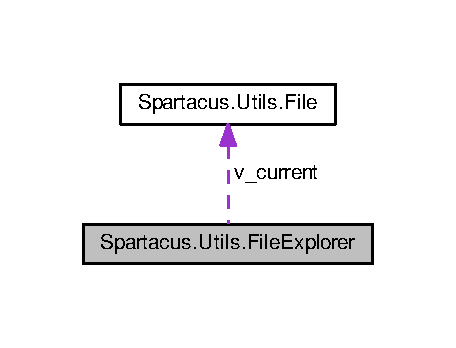
\includegraphics[width=219pt]{classSpartacus_1_1Utils_1_1FileExplorer__coll__graph}
\end{center}
\end{figure}
\subsection*{Métodos Públicos}
\begin{DoxyCompactItemize}
\item 
\hyperlink{classSpartacus_1_1Utils_1_1FileExplorer_a133727a338ccd4e44e9a32c0f89d9852}{File\+Explorer} ()
\begin{DoxyCompactList}\small\item\em Initializa uma nova instância da classe \hyperlink{classSpartacus_1_1Utils_1_1FileExplorer}{Spartacus.\+Utils.\+File\+Explorer}. \end{DoxyCompactList}\item 
\hyperlink{classSpartacus_1_1Utils_1_1FileExplorer_a37f733923b430db407d1459746d7fac7}{File\+Explorer} (string p\+\_\+root)
\begin{DoxyCompactList}\small\item\em Initializa uma nova instância da classe \hyperlink{classSpartacus_1_1Utils_1_1FileExplorer}{Spartacus.\+Utils.\+File\+Explorer}. \end{DoxyCompactList}\item 
\hyperlink{classSpartacus_1_1Utils_1_1FileExplorer_ac9adca2bd6d8767c21aa90a95efb087a}{File\+Explorer} (string p\+\_\+root, \hyperlink{namespaceSpartacus_1_1Utils_a9ee24558a33d60b42674bae3eed2a094}{Spartacus.\+Utils.\+Path\+Separator} p\+\_\+pathseparator)
\begin{DoxyCompactList}\small\item\em Inicializa uma nova instância da classe \hyperlink{classSpartacus_1_1Utils_1_1FileExplorer}{Spartacus.\+Utils.\+File\+Explorer}. \end{DoxyCompactList}\item 
void \hyperlink{classSpartacus_1_1Utils_1_1FileExplorer_a0b21899a7ac47d7a84d0558df390f388}{Set\+Root} (string p\+\_\+root)
\begin{DoxyCompactList}\small\item\em Seta a pasta raiz do explorador de arquivos. \end{DoxyCompactList}\item 
void \hyperlink{classSpartacus_1_1Utils_1_1FileExplorer_afc668f70066735934e76ed84c42b8d7e}{List} ()
\begin{DoxyCompactList}\small\item\em Constrói lista de arquivos e diretorios contidos no diretório atual. \end{DoxyCompactList}\item 
string\mbox{[}$\,$\mbox{]} \hyperlink{classSpartacus_1_1Utils_1_1FileExplorer_a1af76e64b4bb7ff7075179c881c08b71}{Filter\+List} (string p\+\_\+filter, System.\+I\+O.\+Search\+Option p\+\_\+searchoption)
\begin{DoxyCompactList}\small\item\em Lista todos os arquivos cujo nome corresponde ao filtro. O filtro é uma string que pode conter vários filtros separados por '$\vert$'. \end{DoxyCompactList}\item 
void \hyperlink{classSpartacus_1_1Utils_1_1FileExplorer_ac9273b0e7cd1365d67c60b9255e6f538}{Enter} (int p\+\_\+id)
\begin{DoxyCompactList}\small\item\em Entra no diretório especificado. \end{DoxyCompactList}\item 
void \hyperlink{classSpartacus_1_1Utils_1_1FileExplorer_a79d43d93289567d3d0544d9c7b61949e}{Return} ()
\begin{DoxyCompactList}\small\item\em Retorna para o diretório anterior, ou seja, o diretório pai do diretório atual. \end{DoxyCompactList}\item 
\hyperlink{classSpartacus_1_1Utils_1_1File}{Spartacus.\+Utils.\+File} \hyperlink{classSpartacus_1_1Utils_1_1FileExplorer_a75222d9146d14fb15e5fe46b0fa1f3c9}{Get} (int p\+\_\+id)
\begin{DoxyCompactList}\small\item\em Retorna o arquivo ou diretório solicitado de acordo com seu código dentro da lista de arquivos e diretórios. \end{DoxyCompactList}\item 
string \hyperlink{classSpartacus_1_1Utils_1_1FileExplorer_ad6f65e809b0c424f639dde8d6fd5d85f}{Put} (string p\+\_\+file)
\begin{DoxyCompactList}\small\item\em Cria um arquivo. \end{DoxyCompactList}\item 
string \hyperlink{classSpartacus_1_1Utils_1_1FileExplorer_a40dcbbe8a4d5def3f833e528466047b7}{Mkdir} (string p\+\_\+directory)
\begin{DoxyCompactList}\small\item\em Cria um diretório. \end{DoxyCompactList}\item 
void \hyperlink{classSpartacus_1_1Utils_1_1FileExplorer_ac36b8cdbb3a886587a8891d61fa8ed90}{Delete} (int p\+\_\+id)
\begin{DoxyCompactList}\small\item\em Deleta o arquivo ou diretório. \end{DoxyCompactList}\item 
void \hyperlink{classSpartacus_1_1Utils_1_1FileExplorer_a9f4f49e456a17be5e4051a79539b7459}{Filter\+All\+Attributes} (string p\+\_\+completefilter)
\begin{DoxyCompactList}\small\item\em Aplica o filtro do grid A\+J\+A\+X na lista de arquivos. \end{DoxyCompactList}\item 
void \hyperlink{classSpartacus_1_1Utils_1_1FileExplorer_a9d7be5225c56d655c107c0102c86ef12}{Sort\+Attribute} (int p\+\_\+attribute, int p\+\_\+sorttype)
\begin{DoxyCompactList}\small\item\em Ordena a lista de arquivos pela coluna passada como argumento, em ordem ascendente ou descendente. \end{DoxyCompactList}\item 
void \hyperlink{classSpartacus_1_1Utils_1_1FileExplorer_ad56f638a1f11734ca1157f1cdd39c7e7}{Split\+Into\+Pages} (int p\+\_\+numfilesperpage)
\begin{DoxyCompactList}\small\item\em Atribui um número de página a cada arquivo da lista de arquivos e conta o número de páginas. \end{DoxyCompactList}\item 
\hyperlink{classSpartacus_1_1Utils_1_1File}{Spartacus.\+Utils.\+File} \hyperlink{classSpartacus_1_1Utils_1_1FileExplorer_a698a5f476667204c0fbfad527371dca6}{Compress\+Directory} (string p\+\_\+zipfilename, \hyperlink{classSpartacus_1_1Utils_1_1File}{Spartacus.\+Utils.\+File} p\+\_\+directory)
\begin{DoxyCompactList}\small\item\em Cria um arquivo Z\+I\+P a partir de um diretório, no diretório pai do mesmo diretório. \end{DoxyCompactList}\end{DoxyCompactItemize}
\subsection*{Campos de Dados}
\begin{DoxyCompactItemize}
\item 
string \hyperlink{classSpartacus_1_1Utils_1_1FileExplorer_a398279cbdbce816d3c0d40b3dc02eb50}{v\+\_\+root}
\begin{DoxyCompactList}\small\item\em Pasta raiz do explorador de arquivos. \end{DoxyCompactList}\item 
\hyperlink{classSpartacus_1_1Utils_1_1File}{Spartacus.\+Utils.\+File} \hyperlink{classSpartacus_1_1Utils_1_1FileExplorer_a3b9d61aefae4f495fcc4709783671472}{v\+\_\+current}
\begin{DoxyCompactList}\small\item\em Nome da pasta atual. \end{DoxyCompactList}\item 
int \hyperlink{classSpartacus_1_1Utils_1_1FileExplorer_a3622a3fd986d0685ce13c5fe0ebb2c3b}{v\+\_\+currentlevel}
\begin{DoxyCompactList}\small\item\em Nível atual dentro da estrutura de diretórios. \end{DoxyCompactList}\item 
System.\+Collections.\+Array\+List \hyperlink{classSpartacus_1_1Utils_1_1FileExplorer_a94c423e8e9df914fb225b740e4829b11}{v\+\_\+files}
\begin{DoxyCompactList}\small\item\em Lista de arquivos e diretórios da pasta atual. \end{DoxyCompactList}\item 
System.\+Collections.\+Array\+List \hyperlink{classSpartacus_1_1Utils_1_1FileExplorer_adb13bc5f2309ceb21861d1a84caf7f98}{v\+\_\+filesorig}
\begin{DoxyCompactList}\small\item\em Lista original de arquivos e diretórios da pasta atual. \end{DoxyCompactList}\item 
\hyperlink{namespaceSpartacus_1_1Utils_a9ee24558a33d60b42674bae3eed2a094}{Spartacus.\+Utils.\+Path\+Separator} \hyperlink{classSpartacus_1_1Utils_1_1FileExplorer_a566ec72c60a0ddb78eec41f208237d61}{v\+\_\+pathseparator}
\begin{DoxyCompactList}\small\item\em Separador de diretórios. \end{DoxyCompactList}\item 
int \hyperlink{classSpartacus_1_1Utils_1_1FileExplorer_abbf2deab4665a8be42c23393bdbf54df}{v\+\_\+numfilesperpage}
\begin{DoxyCompactList}\small\item\em Número de arquivos por página. \end{DoxyCompactList}\item 
int \hyperlink{classSpartacus_1_1Utils_1_1FileExplorer_a8017af938b655e57eb51eb83fba48ed6}{v\+\_\+numpages}
\begin{DoxyCompactList}\small\item\em Número de páginas. \end{DoxyCompactList}\item 
string \hyperlink{classSpartacus_1_1Utils_1_1FileExplorer_a1e0f31dd0c66b2a6d5003a0ace555eab}{v\+\_\+protectpattern}
\begin{DoxyCompactList}\small\item\em Padrão de nome de arquivo ou diretório que deve ser protegido contra escrita (fictício e não permissões reais do arquivo). \end{DoxyCompactList}\item 
bool \hyperlink{classSpartacus_1_1Utils_1_1FileExplorer_adba2289bce9aadfdbb353f811fa0411c}{v\+\_\+showprotectpattern}
\begin{DoxyCompactList}\small\item\em Informa se a pasta com padrão de proteção deve ser mostrada ou não. \end{DoxyCompactList}\item 
int \hyperlink{classSpartacus_1_1Utils_1_1FileExplorer_a471c35d5854d9f4dbf605da187f262b1}{v\+\_\+protectedminlevel}
\begin{DoxyCompactList}\small\item\em Nível mínimo de proteção de escrita dentro da estrutura de diretórios. \end{DoxyCompactList}\item 
bool \hyperlink{classSpartacus_1_1Utils_1_1FileExplorer_ac0811882d93d76fb122f8aad7ec7b15d}{v\+\_\+showhiddenfiles}
\begin{DoxyCompactList}\small\item\em Informa se arquivos e diretórios ocultos devem ou não ser mostrados. \end{DoxyCompactList}\end{DoxyCompactItemize}


\subsection{Descrição Detalhada}
Classe \hyperlink{classSpartacus_1_1Utils_1_1FileExplorer}{File\+Explorer}. Representa um explorador de arquivos genérico, que pode ser usado em qualquer interface (prompt de comando, desktop ou web). 



\subsection{Construtores \& Destrutores}
\hypertarget{classSpartacus_1_1Utils_1_1FileExplorer_a133727a338ccd4e44e9a32c0f89d9852}{\index{Spartacus\+::\+Utils\+::\+File\+Explorer@{Spartacus\+::\+Utils\+::\+File\+Explorer}!File\+Explorer@{File\+Explorer}}
\index{File\+Explorer@{File\+Explorer}!Spartacus\+::\+Utils\+::\+File\+Explorer@{Spartacus\+::\+Utils\+::\+File\+Explorer}}
\subsubsection[{File\+Explorer}]{\setlength{\rightskip}{0pt plus 5cm}Spartacus.\+Utils.\+File\+Explorer.\+File\+Explorer (
\begin{DoxyParamCaption}
{}
\end{DoxyParamCaption}
)\hspace{0.3cm}{\ttfamily [inline]}}}\label{classSpartacus_1_1Utils_1_1FileExplorer_a133727a338ccd4e44e9a32c0f89d9852}


Initializa uma nova instância da classe \hyperlink{classSpartacus_1_1Utils_1_1FileExplorer}{Spartacus.\+Utils.\+File\+Explorer}. 

\hypertarget{classSpartacus_1_1Utils_1_1FileExplorer_a37f733923b430db407d1459746d7fac7}{\index{Spartacus\+::\+Utils\+::\+File\+Explorer@{Spartacus\+::\+Utils\+::\+File\+Explorer}!File\+Explorer@{File\+Explorer}}
\index{File\+Explorer@{File\+Explorer}!Spartacus\+::\+Utils\+::\+File\+Explorer@{Spartacus\+::\+Utils\+::\+File\+Explorer}}
\subsubsection[{File\+Explorer}]{\setlength{\rightskip}{0pt plus 5cm}Spartacus.\+Utils.\+File\+Explorer.\+File\+Explorer (
\begin{DoxyParamCaption}
\item[{string}]{p\+\_\+root}
\end{DoxyParamCaption}
)\hspace{0.3cm}{\ttfamily [inline]}}}\label{classSpartacus_1_1Utils_1_1FileExplorer_a37f733923b430db407d1459746d7fac7}


Initializa uma nova instância da classe \hyperlink{classSpartacus_1_1Utils_1_1FileExplorer}{Spartacus.\+Utils.\+File\+Explorer}. 


\begin{DoxyParams}{Parâmetros}
{\em p\+\_\+root} & Pasta raiz do explorador de arquivos. \\
\hline
\end{DoxyParams}
\hypertarget{classSpartacus_1_1Utils_1_1FileExplorer_ac9adca2bd6d8767c21aa90a95efb087a}{\index{Spartacus\+::\+Utils\+::\+File\+Explorer@{Spartacus\+::\+Utils\+::\+File\+Explorer}!File\+Explorer@{File\+Explorer}}
\index{File\+Explorer@{File\+Explorer}!Spartacus\+::\+Utils\+::\+File\+Explorer@{Spartacus\+::\+Utils\+::\+File\+Explorer}}
\subsubsection[{File\+Explorer}]{\setlength{\rightskip}{0pt plus 5cm}Spartacus.\+Utils.\+File\+Explorer.\+File\+Explorer (
\begin{DoxyParamCaption}
\item[{string}]{p\+\_\+root, }
\item[{{\bf Spartacus.\+Utils.\+Path\+Separator}}]{p\+\_\+pathseparator}
\end{DoxyParamCaption}
)\hspace{0.3cm}{\ttfamily [inline]}}}\label{classSpartacus_1_1Utils_1_1FileExplorer_ac9adca2bd6d8767c21aa90a95efb087a}


Inicializa uma nova instância da classe \hyperlink{classSpartacus_1_1Utils_1_1FileExplorer}{Spartacus.\+Utils.\+File\+Explorer}. 


\begin{DoxyParams}{Parâmetros}
{\em p\+\_\+root} & Pasta raiz do explorador de arquivos. \\
\hline
{\em p\+\_\+pathseparator} & Separador de diretórios. \\
\hline
\end{DoxyParams}


\subsection{Métodos}
\hypertarget{classSpartacus_1_1Utils_1_1FileExplorer_a698a5f476667204c0fbfad527371dca6}{\index{Spartacus\+::\+Utils\+::\+File\+Explorer@{Spartacus\+::\+Utils\+::\+File\+Explorer}!Compress\+Directory@{Compress\+Directory}}
\index{Compress\+Directory@{Compress\+Directory}!Spartacus\+::\+Utils\+::\+File\+Explorer@{Spartacus\+::\+Utils\+::\+File\+Explorer}}
\subsubsection[{Compress\+Directory}]{\setlength{\rightskip}{0pt plus 5cm}{\bf Spartacus.\+Utils.\+File} Spartacus.\+Utils.\+File\+Explorer.\+Compress\+Directory (
\begin{DoxyParamCaption}
\item[{string}]{p\+\_\+zipfilename, }
\item[{{\bf Spartacus.\+Utils.\+File}}]{p\+\_\+directory}
\end{DoxyParamCaption}
)\hspace{0.3cm}{\ttfamily [inline]}}}\label{classSpartacus_1_1Utils_1_1FileExplorer_a698a5f476667204c0fbfad527371dca6}


Cria um arquivo Z\+I\+P a partir de um diretório, no diretório pai do mesmo diretório. 

\begin{DoxyReturn}{Retorna}
Arquivo Z\+I\+P.
\end{DoxyReturn}

\begin{DoxyParams}{Parâmetros}
{\em p\+\_\+zipfilename} & Nome do arquivo Z\+I\+P a ser criado.\\
\hline
{\em p\+\_\+directory} & Diretório a ser compactado.\\
\hline
\end{DoxyParams}
\hypertarget{classSpartacus_1_1Utils_1_1FileExplorer_ac36b8cdbb3a886587a8891d61fa8ed90}{\index{Spartacus\+::\+Utils\+::\+File\+Explorer@{Spartacus\+::\+Utils\+::\+File\+Explorer}!Delete@{Delete}}
\index{Delete@{Delete}!Spartacus\+::\+Utils\+::\+File\+Explorer@{Spartacus\+::\+Utils\+::\+File\+Explorer}}
\subsubsection[{Delete}]{\setlength{\rightskip}{0pt plus 5cm}void Spartacus.\+Utils.\+File\+Explorer.\+Delete (
\begin{DoxyParamCaption}
\item[{int}]{p\+\_\+id}
\end{DoxyParamCaption}
)\hspace{0.3cm}{\ttfamily [inline]}}}\label{classSpartacus_1_1Utils_1_1FileExplorer_ac36b8cdbb3a886587a8891d61fa8ed90}


Deleta o arquivo ou diretório. 


\begin{DoxyParams}{Parâmetros}
{\em p\+\_\+id} & Código do arquivo dentro da lista de arquivos e diretórios. \\
\hline
\end{DoxyParams}

\begin{DoxyExceptions}{Exceções}
{\em \hyperlink{classSpartacus_1_1Utils_1_1Exception}{Spartacus.\+Utils.\+Exception}} & Exceção acontece quando não é possível remover o arquivo ou diretório.\\
\hline
\end{DoxyExceptions}
\hypertarget{classSpartacus_1_1Utils_1_1FileExplorer_ac9273b0e7cd1365d67c60b9255e6f538}{\index{Spartacus\+::\+Utils\+::\+File\+Explorer@{Spartacus\+::\+Utils\+::\+File\+Explorer}!Enter@{Enter}}
\index{Enter@{Enter}!Spartacus\+::\+Utils\+::\+File\+Explorer@{Spartacus\+::\+Utils\+::\+File\+Explorer}}
\subsubsection[{Enter}]{\setlength{\rightskip}{0pt plus 5cm}void Spartacus.\+Utils.\+File\+Explorer.\+Enter (
\begin{DoxyParamCaption}
\item[{int}]{p\+\_\+id}
\end{DoxyParamCaption}
)\hspace{0.3cm}{\ttfamily [inline]}}}\label{classSpartacus_1_1Utils_1_1FileExplorer_ac9273b0e7cd1365d67c60b9255e6f538}


Entra no diretório especificado. 


\begin{DoxyParams}{Parâmetros}
{\em p\+\_\+id} & Código do diretório dentro da lista de arquivos e diretórios. \\
\hline
\end{DoxyParams}

\begin{DoxyExceptions}{Exceções}
{\em \hyperlink{classSpartacus_1_1Utils_1_1Exception}{Spartacus.\+Utils.\+Exception}} & Exceção acontece quando o item referenciado não é um diretório.\\
\hline
\end{DoxyExceptions}
\hypertarget{classSpartacus_1_1Utils_1_1FileExplorer_a9f4f49e456a17be5e4051a79539b7459}{\index{Spartacus\+::\+Utils\+::\+File\+Explorer@{Spartacus\+::\+Utils\+::\+File\+Explorer}!Filter\+All\+Attributes@{Filter\+All\+Attributes}}
\index{Filter\+All\+Attributes@{Filter\+All\+Attributes}!Spartacus\+::\+Utils\+::\+File\+Explorer@{Spartacus\+::\+Utils\+::\+File\+Explorer}}
\subsubsection[{Filter\+All\+Attributes}]{\setlength{\rightskip}{0pt plus 5cm}void Spartacus.\+Utils.\+File\+Explorer.\+Filter\+All\+Attributes (
\begin{DoxyParamCaption}
\item[{string}]{p\+\_\+completefilter}
\end{DoxyParamCaption}
)\hspace{0.3cm}{\ttfamily [inline]}}}\label{classSpartacus_1_1Utils_1_1FileExplorer_a9f4f49e456a17be5e4051a79539b7459}


Aplica o filtro do grid A\+J\+A\+X na lista de arquivos. 


\begin{DoxyParams}{Parâmetros}
{\em p\+\_\+completefilter} & Filtro completo com valores separados por '\&'.\\
\hline
\end{DoxyParams}
\hypertarget{classSpartacus_1_1Utils_1_1FileExplorer_a1af76e64b4bb7ff7075179c881c08b71}{\index{Spartacus\+::\+Utils\+::\+File\+Explorer@{Spartacus\+::\+Utils\+::\+File\+Explorer}!Filter\+List@{Filter\+List}}
\index{Filter\+List@{Filter\+List}!Spartacus\+::\+Utils\+::\+File\+Explorer@{Spartacus\+::\+Utils\+::\+File\+Explorer}}
\subsubsection[{Filter\+List}]{\setlength{\rightskip}{0pt plus 5cm}string \mbox{[}$\,$\mbox{]} Spartacus.\+Utils.\+File\+Explorer.\+Filter\+List (
\begin{DoxyParamCaption}
\item[{string}]{p\+\_\+filter, }
\item[{System.\+I\+O.\+Search\+Option}]{p\+\_\+searchoption}
\end{DoxyParamCaption}
)\hspace{0.3cm}{\ttfamily [inline]}}}\label{classSpartacus_1_1Utils_1_1FileExplorer_a1af76e64b4bb7ff7075179c881c08b71}


Lista todos os arquivos cujo nome corresponde ao filtro. O filtro é uma string que pode conter vários filtros separados por '$\vert$'. 

\begin{DoxyReturn}{Retorna}
Lista com o nome completo de todos os arquivos que correspondem ao filtro.
\end{DoxyReturn}

\begin{DoxyParams}{Parâmetros}
{\em p\+\_\+filter} & String que pode conter vários filtros separados por '$\vert$'.\\
\hline
{\em p\+\_\+searchoption} & Opção de busca.\\
\hline
\end{DoxyParams}
\hypertarget{classSpartacus_1_1Utils_1_1FileExplorer_a75222d9146d14fb15e5fe46b0fa1f3c9}{\index{Spartacus\+::\+Utils\+::\+File\+Explorer@{Spartacus\+::\+Utils\+::\+File\+Explorer}!Get@{Get}}
\index{Get@{Get}!Spartacus\+::\+Utils\+::\+File\+Explorer@{Spartacus\+::\+Utils\+::\+File\+Explorer}}
\subsubsection[{Get}]{\setlength{\rightskip}{0pt plus 5cm}{\bf Spartacus.\+Utils.\+File} Spartacus.\+Utils.\+File\+Explorer.\+Get (
\begin{DoxyParamCaption}
\item[{int}]{p\+\_\+id}
\end{DoxyParamCaption}
)\hspace{0.3cm}{\ttfamily [inline]}}}\label{classSpartacus_1_1Utils_1_1FileExplorer_a75222d9146d14fb15e5fe46b0fa1f3c9}


Retorna o arquivo ou diretório solicitado de acordo com seu código dentro da lista de arquivos e diretórios. 

\begin{DoxyReturn}{Retorna}
Arquivo ou diretório especificado. 
\end{DoxyReturn}

\begin{DoxyParams}{Parâmetros}
{\em p\+\_\+id} & Código do arquivo ou diretório dentro da lista de arquivos e diretórios. \\
\hline
\end{DoxyParams}
\hypertarget{classSpartacus_1_1Utils_1_1FileExplorer_afc668f70066735934e76ed84c42b8d7e}{\index{Spartacus\+::\+Utils\+::\+File\+Explorer@{Spartacus\+::\+Utils\+::\+File\+Explorer}!List@{List}}
\index{List@{List}!Spartacus\+::\+Utils\+::\+File\+Explorer@{Spartacus\+::\+Utils\+::\+File\+Explorer}}
\subsubsection[{List}]{\setlength{\rightskip}{0pt plus 5cm}void Spartacus.\+Utils.\+File\+Explorer.\+List (
\begin{DoxyParamCaption}
{}
\end{DoxyParamCaption}
)\hspace{0.3cm}{\ttfamily [inline]}}}\label{classSpartacus_1_1Utils_1_1FileExplorer_afc668f70066735934e76ed84c42b8d7e}


Constrói lista de arquivos e diretorios contidos no diretório atual. 


\begin{DoxyExceptions}{Exceções}
{\em \hyperlink{classSpartacus_1_1Utils_1_1Exception}{Spartacus.\+Utils.\+Exception}} & Exceção acontece quando não conseguir listar o conteúdo do diretório atual.\\
\hline
\end{DoxyExceptions}
\hypertarget{classSpartacus_1_1Utils_1_1FileExplorer_a40dcbbe8a4d5def3f833e528466047b7}{\index{Spartacus\+::\+Utils\+::\+File\+Explorer@{Spartacus\+::\+Utils\+::\+File\+Explorer}!Mkdir@{Mkdir}}
\index{Mkdir@{Mkdir}!Spartacus\+::\+Utils\+::\+File\+Explorer@{Spartacus\+::\+Utils\+::\+File\+Explorer}}
\subsubsection[{Mkdir}]{\setlength{\rightskip}{0pt plus 5cm}string Spartacus.\+Utils.\+File\+Explorer.\+Mkdir (
\begin{DoxyParamCaption}
\item[{string}]{p\+\_\+directory}
\end{DoxyParamCaption}
)\hspace{0.3cm}{\ttfamily [inline]}}}\label{classSpartacus_1_1Utils_1_1FileExplorer_a40dcbbe8a4d5def3f833e528466047b7}


Cria um diretório. 

\begin{DoxyReturn}{Retorna}
Nome completo do novo diretório a ser criado. 
\end{DoxyReturn}

\begin{DoxyParams}{Parâmetros}
{\em p\+\_\+directory} & Nome do novo diretório a ser criado. \\
\hline
\end{DoxyParams}

\begin{DoxyExceptions}{Exceções}
{\em \hyperlink{classSpartacus_1_1Utils_1_1Exception}{Spartacus.\+Utils.\+Exception}} & Exceção acontece quando não é possível criar o diretório.\\
\hline
\end{DoxyExceptions}
\hypertarget{classSpartacus_1_1Utils_1_1FileExplorer_ad6f65e809b0c424f639dde8d6fd5d85f}{\index{Spartacus\+::\+Utils\+::\+File\+Explorer@{Spartacus\+::\+Utils\+::\+File\+Explorer}!Put@{Put}}
\index{Put@{Put}!Spartacus\+::\+Utils\+::\+File\+Explorer@{Spartacus\+::\+Utils\+::\+File\+Explorer}}
\subsubsection[{Put}]{\setlength{\rightskip}{0pt plus 5cm}string Spartacus.\+Utils.\+File\+Explorer.\+Put (
\begin{DoxyParamCaption}
\item[{string}]{p\+\_\+file}
\end{DoxyParamCaption}
)\hspace{0.3cm}{\ttfamily [inline]}}}\label{classSpartacus_1_1Utils_1_1FileExplorer_ad6f65e809b0c424f639dde8d6fd5d85f}


Cria um arquivo. 

\begin{DoxyReturn}{Retorna}
Nome completo do novo arquivo a ser criado. 
\end{DoxyReturn}

\begin{DoxyParams}{Parâmetros}
{\em p\+\_\+file} & Nome do novo arquivo a ser criado. \\
\hline
\end{DoxyParams}

\begin{DoxyExceptions}{Exceções}
{\em \hyperlink{classSpartacus_1_1Utils_1_1Exception}{Spartacus.\+Utils.\+Exception}} & Exceção acontece quando não é possível criar o arquivo.\\
\hline
\end{DoxyExceptions}
\hypertarget{classSpartacus_1_1Utils_1_1FileExplorer_a79d43d93289567d3d0544d9c7b61949e}{\index{Spartacus\+::\+Utils\+::\+File\+Explorer@{Spartacus\+::\+Utils\+::\+File\+Explorer}!Return@{Return}}
\index{Return@{Return}!Spartacus\+::\+Utils\+::\+File\+Explorer@{Spartacus\+::\+Utils\+::\+File\+Explorer}}
\subsubsection[{Return}]{\setlength{\rightskip}{0pt plus 5cm}void Spartacus.\+Utils.\+File\+Explorer.\+Return (
\begin{DoxyParamCaption}
{}
\end{DoxyParamCaption}
)\hspace{0.3cm}{\ttfamily [inline]}}}\label{classSpartacus_1_1Utils_1_1FileExplorer_a79d43d93289567d3d0544d9c7b61949e}


Retorna para o diretório anterior, ou seja, o diretório pai do diretório atual. 


\begin{DoxyExceptions}{Exceções}
{\em \hyperlink{classSpartacus_1_1Utils_1_1Exception}{Spartacus.\+Utils.\+Exception}} & Exceção acontece quando o diretório atual também é a raiz do explorador de arquivos.\\
\hline
\end{DoxyExceptions}
\hypertarget{classSpartacus_1_1Utils_1_1FileExplorer_a0b21899a7ac47d7a84d0558df390f388}{\index{Spartacus\+::\+Utils\+::\+File\+Explorer@{Spartacus\+::\+Utils\+::\+File\+Explorer}!Set\+Root@{Set\+Root}}
\index{Set\+Root@{Set\+Root}!Spartacus\+::\+Utils\+::\+File\+Explorer@{Spartacus\+::\+Utils\+::\+File\+Explorer}}
\subsubsection[{Set\+Root}]{\setlength{\rightskip}{0pt plus 5cm}void Spartacus.\+Utils.\+File\+Explorer.\+Set\+Root (
\begin{DoxyParamCaption}
\item[{string}]{p\+\_\+root}
\end{DoxyParamCaption}
)\hspace{0.3cm}{\ttfamily [inline]}}}\label{classSpartacus_1_1Utils_1_1FileExplorer_a0b21899a7ac47d7a84d0558df390f388}


Seta a pasta raiz do explorador de arquivos. 


\begin{DoxyParams}{Parâmetros}
{\em p\+\_\+root} & Pasta raiz do explorador de arquivos. \\
\hline
\end{DoxyParams}
\hypertarget{classSpartacus_1_1Utils_1_1FileExplorer_a9d7be5225c56d655c107c0102c86ef12}{\index{Spartacus\+::\+Utils\+::\+File\+Explorer@{Spartacus\+::\+Utils\+::\+File\+Explorer}!Sort\+Attribute@{Sort\+Attribute}}
\index{Sort\+Attribute@{Sort\+Attribute}!Spartacus\+::\+Utils\+::\+File\+Explorer@{Spartacus\+::\+Utils\+::\+File\+Explorer}}
\subsubsection[{Sort\+Attribute}]{\setlength{\rightskip}{0pt plus 5cm}void Spartacus.\+Utils.\+File\+Explorer.\+Sort\+Attribute (
\begin{DoxyParamCaption}
\item[{int}]{p\+\_\+attribute, }
\item[{int}]{p\+\_\+sorttype}
\end{DoxyParamCaption}
)\hspace{0.3cm}{\ttfamily [inline]}}}\label{classSpartacus_1_1Utils_1_1FileExplorer_a9d7be5225c56d655c107c0102c86ef12}


Ordena a lista de arquivos pela coluna passada como argumento, em ordem ascendente ou descendente. 


\begin{DoxyParams}{Parâmetros}
{\em p\+\_\+attribute} & Coluna a ser ordenada (1, 2, 3, 4, 5 ou 6).\\
\hline
{\em p\+\_\+sorttype} & Ordem (1\+: Ascendente ou 2\+: Descendente).\\
\hline
\end{DoxyParams}
\hypertarget{classSpartacus_1_1Utils_1_1FileExplorer_ad56f638a1f11734ca1157f1cdd39c7e7}{\index{Spartacus\+::\+Utils\+::\+File\+Explorer@{Spartacus\+::\+Utils\+::\+File\+Explorer}!Split\+Into\+Pages@{Split\+Into\+Pages}}
\index{Split\+Into\+Pages@{Split\+Into\+Pages}!Spartacus\+::\+Utils\+::\+File\+Explorer@{Spartacus\+::\+Utils\+::\+File\+Explorer}}
\subsubsection[{Split\+Into\+Pages}]{\setlength{\rightskip}{0pt plus 5cm}void Spartacus.\+Utils.\+File\+Explorer.\+Split\+Into\+Pages (
\begin{DoxyParamCaption}
\item[{int}]{p\+\_\+numfilesperpage}
\end{DoxyParamCaption}
)\hspace{0.3cm}{\ttfamily [inline]}}}\label{classSpartacus_1_1Utils_1_1FileExplorer_ad56f638a1f11734ca1157f1cdd39c7e7}


Atribui um número de página a cada arquivo da lista de arquivos e conta o número de páginas. 


\begin{DoxyParams}{Parâmetros}
{\em p\+\_\+numfilesperpage} & Número de arquivos por página.\\
\hline
\end{DoxyParams}


\subsection{Campos}
\hypertarget{classSpartacus_1_1Utils_1_1FileExplorer_a3b9d61aefae4f495fcc4709783671472}{\index{Spartacus\+::\+Utils\+::\+File\+Explorer@{Spartacus\+::\+Utils\+::\+File\+Explorer}!v\+\_\+current@{v\+\_\+current}}
\index{v\+\_\+current@{v\+\_\+current}!Spartacus\+::\+Utils\+::\+File\+Explorer@{Spartacus\+::\+Utils\+::\+File\+Explorer}}
\subsubsection[{v\+\_\+current}]{\setlength{\rightskip}{0pt plus 5cm}{\bf Spartacus.\+Utils.\+File} Spartacus.\+Utils.\+File\+Explorer.\+v\+\_\+current}}\label{classSpartacus_1_1Utils_1_1FileExplorer_a3b9d61aefae4f495fcc4709783671472}


Nome da pasta atual. 

\hypertarget{classSpartacus_1_1Utils_1_1FileExplorer_a3622a3fd986d0685ce13c5fe0ebb2c3b}{\index{Spartacus\+::\+Utils\+::\+File\+Explorer@{Spartacus\+::\+Utils\+::\+File\+Explorer}!v\+\_\+currentlevel@{v\+\_\+currentlevel}}
\index{v\+\_\+currentlevel@{v\+\_\+currentlevel}!Spartacus\+::\+Utils\+::\+File\+Explorer@{Spartacus\+::\+Utils\+::\+File\+Explorer}}
\subsubsection[{v\+\_\+currentlevel}]{\setlength{\rightskip}{0pt plus 5cm}int Spartacus.\+Utils.\+File\+Explorer.\+v\+\_\+currentlevel}}\label{classSpartacus_1_1Utils_1_1FileExplorer_a3622a3fd986d0685ce13c5fe0ebb2c3b}


Nível atual dentro da estrutura de diretórios. 

\hypertarget{classSpartacus_1_1Utils_1_1FileExplorer_a94c423e8e9df914fb225b740e4829b11}{\index{Spartacus\+::\+Utils\+::\+File\+Explorer@{Spartacus\+::\+Utils\+::\+File\+Explorer}!v\+\_\+files@{v\+\_\+files}}
\index{v\+\_\+files@{v\+\_\+files}!Spartacus\+::\+Utils\+::\+File\+Explorer@{Spartacus\+::\+Utils\+::\+File\+Explorer}}
\subsubsection[{v\+\_\+files}]{\setlength{\rightskip}{0pt plus 5cm}System.\+Collections.\+Array\+List Spartacus.\+Utils.\+File\+Explorer.\+v\+\_\+files}}\label{classSpartacus_1_1Utils_1_1FileExplorer_a94c423e8e9df914fb225b740e4829b11}


Lista de arquivos e diretórios da pasta atual. 

\hypertarget{classSpartacus_1_1Utils_1_1FileExplorer_adb13bc5f2309ceb21861d1a84caf7f98}{\index{Spartacus\+::\+Utils\+::\+File\+Explorer@{Spartacus\+::\+Utils\+::\+File\+Explorer}!v\+\_\+filesorig@{v\+\_\+filesorig}}
\index{v\+\_\+filesorig@{v\+\_\+filesorig}!Spartacus\+::\+Utils\+::\+File\+Explorer@{Spartacus\+::\+Utils\+::\+File\+Explorer}}
\subsubsection[{v\+\_\+filesorig}]{\setlength{\rightskip}{0pt plus 5cm}System.\+Collections.\+Array\+List Spartacus.\+Utils.\+File\+Explorer.\+v\+\_\+filesorig}}\label{classSpartacus_1_1Utils_1_1FileExplorer_adb13bc5f2309ceb21861d1a84caf7f98}


Lista original de arquivos e diretórios da pasta atual. 

\hypertarget{classSpartacus_1_1Utils_1_1FileExplorer_abbf2deab4665a8be42c23393bdbf54df}{\index{Spartacus\+::\+Utils\+::\+File\+Explorer@{Spartacus\+::\+Utils\+::\+File\+Explorer}!v\+\_\+numfilesperpage@{v\+\_\+numfilesperpage}}
\index{v\+\_\+numfilesperpage@{v\+\_\+numfilesperpage}!Spartacus\+::\+Utils\+::\+File\+Explorer@{Spartacus\+::\+Utils\+::\+File\+Explorer}}
\subsubsection[{v\+\_\+numfilesperpage}]{\setlength{\rightskip}{0pt plus 5cm}int Spartacus.\+Utils.\+File\+Explorer.\+v\+\_\+numfilesperpage}}\label{classSpartacus_1_1Utils_1_1FileExplorer_abbf2deab4665a8be42c23393bdbf54df}


Número de arquivos por página. 

\hypertarget{classSpartacus_1_1Utils_1_1FileExplorer_a8017af938b655e57eb51eb83fba48ed6}{\index{Spartacus\+::\+Utils\+::\+File\+Explorer@{Spartacus\+::\+Utils\+::\+File\+Explorer}!v\+\_\+numpages@{v\+\_\+numpages}}
\index{v\+\_\+numpages@{v\+\_\+numpages}!Spartacus\+::\+Utils\+::\+File\+Explorer@{Spartacus\+::\+Utils\+::\+File\+Explorer}}
\subsubsection[{v\+\_\+numpages}]{\setlength{\rightskip}{0pt plus 5cm}int Spartacus.\+Utils.\+File\+Explorer.\+v\+\_\+numpages}}\label{classSpartacus_1_1Utils_1_1FileExplorer_a8017af938b655e57eb51eb83fba48ed6}


Número de páginas. 

\hypertarget{classSpartacus_1_1Utils_1_1FileExplorer_a566ec72c60a0ddb78eec41f208237d61}{\index{Spartacus\+::\+Utils\+::\+File\+Explorer@{Spartacus\+::\+Utils\+::\+File\+Explorer}!v\+\_\+pathseparator@{v\+\_\+pathseparator}}
\index{v\+\_\+pathseparator@{v\+\_\+pathseparator}!Spartacus\+::\+Utils\+::\+File\+Explorer@{Spartacus\+::\+Utils\+::\+File\+Explorer}}
\subsubsection[{v\+\_\+pathseparator}]{\setlength{\rightskip}{0pt plus 5cm}{\bf Spartacus.\+Utils.\+Path\+Separator} Spartacus.\+Utils.\+File\+Explorer.\+v\+\_\+pathseparator}}\label{classSpartacus_1_1Utils_1_1FileExplorer_a566ec72c60a0ddb78eec41f208237d61}


Separador de diretórios. 

\hypertarget{classSpartacus_1_1Utils_1_1FileExplorer_a471c35d5854d9f4dbf605da187f262b1}{\index{Spartacus\+::\+Utils\+::\+File\+Explorer@{Spartacus\+::\+Utils\+::\+File\+Explorer}!v\+\_\+protectedminlevel@{v\+\_\+protectedminlevel}}
\index{v\+\_\+protectedminlevel@{v\+\_\+protectedminlevel}!Spartacus\+::\+Utils\+::\+File\+Explorer@{Spartacus\+::\+Utils\+::\+File\+Explorer}}
\subsubsection[{v\+\_\+protectedminlevel}]{\setlength{\rightskip}{0pt plus 5cm}int Spartacus.\+Utils.\+File\+Explorer.\+v\+\_\+protectedminlevel}}\label{classSpartacus_1_1Utils_1_1FileExplorer_a471c35d5854d9f4dbf605da187f262b1}


Nível mínimo de proteção de escrita dentro da estrutura de diretórios. 

\hypertarget{classSpartacus_1_1Utils_1_1FileExplorer_a1e0f31dd0c66b2a6d5003a0ace555eab}{\index{Spartacus\+::\+Utils\+::\+File\+Explorer@{Spartacus\+::\+Utils\+::\+File\+Explorer}!v\+\_\+protectpattern@{v\+\_\+protectpattern}}
\index{v\+\_\+protectpattern@{v\+\_\+protectpattern}!Spartacus\+::\+Utils\+::\+File\+Explorer@{Spartacus\+::\+Utils\+::\+File\+Explorer}}
\subsubsection[{v\+\_\+protectpattern}]{\setlength{\rightskip}{0pt plus 5cm}string Spartacus.\+Utils.\+File\+Explorer.\+v\+\_\+protectpattern}}\label{classSpartacus_1_1Utils_1_1FileExplorer_a1e0f31dd0c66b2a6d5003a0ace555eab}


Padrão de nome de arquivo ou diretório que deve ser protegido contra escrita (fictício e não permissões reais do arquivo). 

\hypertarget{classSpartacus_1_1Utils_1_1FileExplorer_a398279cbdbce816d3c0d40b3dc02eb50}{\index{Spartacus\+::\+Utils\+::\+File\+Explorer@{Spartacus\+::\+Utils\+::\+File\+Explorer}!v\+\_\+root@{v\+\_\+root}}
\index{v\+\_\+root@{v\+\_\+root}!Spartacus\+::\+Utils\+::\+File\+Explorer@{Spartacus\+::\+Utils\+::\+File\+Explorer}}
\subsubsection[{v\+\_\+root}]{\setlength{\rightskip}{0pt plus 5cm}string Spartacus.\+Utils.\+File\+Explorer.\+v\+\_\+root}}\label{classSpartacus_1_1Utils_1_1FileExplorer_a398279cbdbce816d3c0d40b3dc02eb50}


Pasta raiz do explorador de arquivos. 

\hypertarget{classSpartacus_1_1Utils_1_1FileExplorer_ac0811882d93d76fb122f8aad7ec7b15d}{\index{Spartacus\+::\+Utils\+::\+File\+Explorer@{Spartacus\+::\+Utils\+::\+File\+Explorer}!v\+\_\+showhiddenfiles@{v\+\_\+showhiddenfiles}}
\index{v\+\_\+showhiddenfiles@{v\+\_\+showhiddenfiles}!Spartacus\+::\+Utils\+::\+File\+Explorer@{Spartacus\+::\+Utils\+::\+File\+Explorer}}
\subsubsection[{v\+\_\+showhiddenfiles}]{\setlength{\rightskip}{0pt plus 5cm}bool Spartacus.\+Utils.\+File\+Explorer.\+v\+\_\+showhiddenfiles}}\label{classSpartacus_1_1Utils_1_1FileExplorer_ac0811882d93d76fb122f8aad7ec7b15d}


Informa se arquivos e diretórios ocultos devem ou não ser mostrados. 

\hypertarget{classSpartacus_1_1Utils_1_1FileExplorer_adba2289bce9aadfdbb353f811fa0411c}{\index{Spartacus\+::\+Utils\+::\+File\+Explorer@{Spartacus\+::\+Utils\+::\+File\+Explorer}!v\+\_\+showprotectpattern@{v\+\_\+showprotectpattern}}
\index{v\+\_\+showprotectpattern@{v\+\_\+showprotectpattern}!Spartacus\+::\+Utils\+::\+File\+Explorer@{Spartacus\+::\+Utils\+::\+File\+Explorer}}
\subsubsection[{v\+\_\+showprotectpattern}]{\setlength{\rightskip}{0pt plus 5cm}bool Spartacus.\+Utils.\+File\+Explorer.\+v\+\_\+showprotectpattern}}\label{classSpartacus_1_1Utils_1_1FileExplorer_adba2289bce9aadfdbb353f811fa0411c}


Informa se a pasta com padrão de proteção deve ser mostrada ou não. 



A documentação para esta classe foi gerada a partir do seguinte arquivo\+:\begin{DoxyCompactItemize}
\item 
Spartacus.\+Utils.\+File\+Explorer.\+cs\end{DoxyCompactItemize}

\hypertarget{classSpartacus_1_1Database_1_1Firebird}{\section{Referência da Classe Spartacus.\+Database.\+Firebird}
\label{classSpartacus_1_1Database_1_1Firebird}\index{Spartacus.\+Database.\+Firebird@{Spartacus.\+Database.\+Firebird}}
}


Classe \hyperlink{classSpartacus_1_1Database_1_1Firebird}{Spartacus.\+Database.\+Firebird}. Herda da classe \hyperlink{classSpartacus_1_1Database_1_1Generic}{Spartacus.\+Database.\+Generic}. Utiliza o \hyperlink{classSpartacus_1_1Database_1_1Firebird}{Firebird} .N\+E\+T Provider para acessar um S\+G\+B\+D \hyperlink{classSpartacus_1_1Database_1_1Firebird}{Firebird}.  




Diagrama de Hierarquia para Spartacus.\+Database.\+Firebird\+:\nopagebreak
\begin{figure}[H]
\begin{center}
\leavevmode
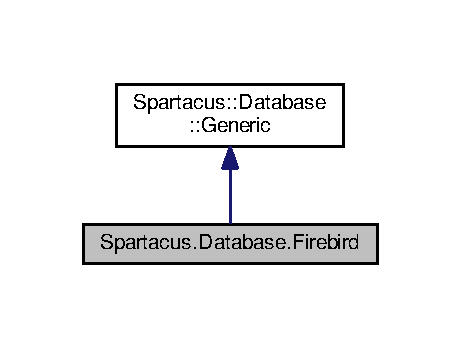
\includegraphics[width=221pt]{classSpartacus_1_1Database_1_1Firebird__inherit__graph}
\end{center}
\end{figure}


Diagrama de colaboração para Spartacus.\+Database.\+Firebird\+:\nopagebreak
\begin{figure}[H]
\begin{center}
\leavevmode
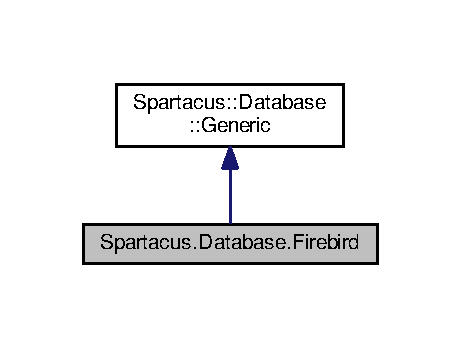
\includegraphics[width=221pt]{classSpartacus_1_1Database_1_1Firebird__coll__graph}
\end{center}
\end{figure}
\subsection*{Métodos Públicos}
\begin{DoxyCompactItemize}
\item 
\hyperlink{classSpartacus_1_1Database_1_1Firebird_ad561c2ad372a44fc785238e72dbc10b4}{Firebird} (string p\+\_\+source, string p\+\_\+port, string p\+\_\+file, string p\+\_\+user, string p\+\_\+password)
\begin{DoxyCompactList}\small\item\em Inicializa uma nova instancia da classe \hyperlink{classSpartacus_1_1Database_1_1Firebird}{Spartacus.\+Database.\+Firebird}. \end{DoxyCompactList}\item 
override System.\+Data.\+Data\+Table \hyperlink{classSpartacus_1_1Database_1_1Firebird_a10235140b612dd5b178169461962d2df}{Query} (string p\+\_\+sql, string p\+\_\+tablename)
\begin{DoxyCompactList}\small\item\em Realiza uma consulta no banco de dados, armazenando os dados de retorno em um System.\+Data.\+Data\+Table. \end{DoxyCompactList}\item 
override System.\+Data.\+Data\+Table \hyperlink{classSpartacus_1_1Database_1_1Firebird_a6243d18345e2b5f44ddcda032f6b2b9e}{Query} (string p\+\_\+sql, string p\+\_\+tablename, System.\+Data.\+Data\+Table p\+\_\+table)
\begin{DoxyCompactList}\small\item\em Realiza uma consulta no banco de dados, armazenando os dados de retorno em um System.\+Data.\+Data\+Table. \end{DoxyCompactList}\item 
override void \hyperlink{classSpartacus_1_1Database_1_1Firebird_a1844a94a27db40450a91a1d415a9d456}{Execute} (string p\+\_\+sql)
\begin{DoxyCompactList}\small\item\em Executa um código S\+Q\+L no banco de dados. \end{DoxyCompactList}\item 
override string \hyperlink{classSpartacus_1_1Database_1_1Firebird_ab785abbc3e5f8b989c10c3a771981a83}{Execute\+Scalar} (string p\+\_\+sql)
\begin{DoxyCompactList}\small\item\em Realiza uma consulta no banco de dados, armazenando um único dado de retorno em uma string. \end{DoxyCompactList}\end{DoxyCompactItemize}
\subsection*{Campos de Dados}
\begin{DoxyCompactItemize}
\item 
string \hyperlink{classSpartacus_1_1Database_1_1Firebird_afb3d04d42e84e18c12d75bed71fb0b45}{v\+\_\+connectionstring}
\begin{DoxyCompactList}\small\item\em String de conexão para acessar o banco. \end{DoxyCompactList}\end{DoxyCompactItemize}


\subsection{Descrição Detalhada}
Classe \hyperlink{classSpartacus_1_1Database_1_1Firebird}{Spartacus.\+Database.\+Firebird}. Herda da classe \hyperlink{classSpartacus_1_1Database_1_1Generic}{Spartacus.\+Database.\+Generic}. Utiliza o \hyperlink{classSpartacus_1_1Database_1_1Firebird}{Firebird} .N\+E\+T Provider para acessar um S\+G\+B\+D \hyperlink{classSpartacus_1_1Database_1_1Firebird}{Firebird}. 



\subsection{Construtores \& Destrutores}
\hypertarget{classSpartacus_1_1Database_1_1Firebird_ad561c2ad372a44fc785238e72dbc10b4}{\index{Spartacus\+::\+Database\+::\+Firebird@{Spartacus\+::\+Database\+::\+Firebird}!Firebird@{Firebird}}
\index{Firebird@{Firebird}!Spartacus\+::\+Database\+::\+Firebird@{Spartacus\+::\+Database\+::\+Firebird}}
\subsubsection[{Firebird}]{\setlength{\rightskip}{0pt plus 5cm}Spartacus.\+Database.\+Firebird.\+Firebird (
\begin{DoxyParamCaption}
\item[{string}]{p\+\_\+source, }
\item[{string}]{p\+\_\+port, }
\item[{string}]{p\+\_\+file, }
\item[{string}]{p\+\_\+user, }
\item[{string}]{p\+\_\+password}
\end{DoxyParamCaption}
)\hspace{0.3cm}{\ttfamily [inline]}}}\label{classSpartacus_1_1Database_1_1Firebird_ad561c2ad372a44fc785238e72dbc10b4}


Inicializa uma nova instancia da classe \hyperlink{classSpartacus_1_1Database_1_1Firebird}{Spartacus.\+Database.\+Firebird}. 


\begin{DoxyParams}{Parâmetros}
{\em p\+\_\+source} & I\+P do servidor \hyperlink{classSpartacus_1_1Database_1_1Firebird}{Firebird}. \\
\hline
{\em p\+\_\+port} & Porta de conexão. \\
\hline
{\em p\+\_\+file} & Caminho completo para o arquivo F\+D\+B ou G\+D\+B. \\
\hline
{\em p\+\_\+user} & Usuário do \hyperlink{classSpartacus_1_1Database_1_1Firebird}{Firebird}. \\
\hline
{\em p\+\_\+password} & Senha do \hyperlink{classSpartacus_1_1Database_1_1Firebird}{Firebird}. \\
\hline
\end{DoxyParams}


\subsection{Métodos}
\hypertarget{classSpartacus_1_1Database_1_1Firebird_a1844a94a27db40450a91a1d415a9d456}{\index{Spartacus\+::\+Database\+::\+Firebird@{Spartacus\+::\+Database\+::\+Firebird}!Execute@{Execute}}
\index{Execute@{Execute}!Spartacus\+::\+Database\+::\+Firebird@{Spartacus\+::\+Database\+::\+Firebird}}
\subsubsection[{Execute}]{\setlength{\rightskip}{0pt plus 5cm}override void Spartacus.\+Database.\+Firebird.\+Execute (
\begin{DoxyParamCaption}
\item[{string}]{p\+\_\+sql}
\end{DoxyParamCaption}
)\hspace{0.3cm}{\ttfamily [inline]}, {\ttfamily [virtual]}}}\label{classSpartacus_1_1Database_1_1Firebird_a1844a94a27db40450a91a1d415a9d456}


Executa um código S\+Q\+L no banco de dados. 


\begin{DoxyParams}{Parâmetros}
{\em p\+\_\+sql} & Código S\+Q\+L a ser executado no banco de dados. \\
\hline
\end{DoxyParams}

\begin{DoxyExceptions}{Exceções}
{\em \hyperlink{classSpartacus_1_1Database_1_1Exception}{Spartacus.\+Database.\+Exception}} & Exceção acontece quando não for possível executar o código S\+Q\+L.\\
\hline
\end{DoxyExceptions}


Implementa \hyperlink{classSpartacus_1_1Database_1_1Generic_a28f1c8821906653eb4ff1484de893d16}{Spartacus.\+Database.\+Generic}.

\hypertarget{classSpartacus_1_1Database_1_1Firebird_ab785abbc3e5f8b989c10c3a771981a83}{\index{Spartacus\+::\+Database\+::\+Firebird@{Spartacus\+::\+Database\+::\+Firebird}!Execute\+Scalar@{Execute\+Scalar}}
\index{Execute\+Scalar@{Execute\+Scalar}!Spartacus\+::\+Database\+::\+Firebird@{Spartacus\+::\+Database\+::\+Firebird}}
\subsubsection[{Execute\+Scalar}]{\setlength{\rightskip}{0pt plus 5cm}override string Spartacus.\+Database.\+Firebird.\+Execute\+Scalar (
\begin{DoxyParamCaption}
\item[{string}]{p\+\_\+sql}
\end{DoxyParamCaption}
)\hspace{0.3cm}{\ttfamily [inline]}, {\ttfamily [virtual]}}}\label{classSpartacus_1_1Database_1_1Firebird_ab785abbc3e5f8b989c10c3a771981a83}


Realiza uma consulta no banco de dados, armazenando um único dado de retorno em uma string. 

\begin{DoxyReturn}{Retorna}
string com o dado de retorno. 
\end{DoxyReturn}

\begin{DoxyParams}{Parâmetros}
{\em p\+\_\+sql} & Código S\+Q\+L a ser consultado no banco de dados. \\
\hline
\end{DoxyParams}

\begin{DoxyExceptions}{Exceções}
{\em \hyperlink{classSpartacus_1_1Database_1_1Exception}{Spartacus.\+Database.\+Exception}} & Exceção acontece quando não for possível executar o código S\+Q\+L.\\
\hline
\end{DoxyExceptions}


Implementa \hyperlink{classSpartacus_1_1Database_1_1Generic_a983620fd71f520deb71ae55304b98bf6}{Spartacus.\+Database.\+Generic}.

\hypertarget{classSpartacus_1_1Database_1_1Firebird_a10235140b612dd5b178169461962d2df}{\index{Spartacus\+::\+Database\+::\+Firebird@{Spartacus\+::\+Database\+::\+Firebird}!Query@{Query}}
\index{Query@{Query}!Spartacus\+::\+Database\+::\+Firebird@{Spartacus\+::\+Database\+::\+Firebird}}
\subsubsection[{Query}]{\setlength{\rightskip}{0pt plus 5cm}override System.\+Data.\+Data\+Table Spartacus.\+Database.\+Firebird.\+Query (
\begin{DoxyParamCaption}
\item[{string}]{p\+\_\+sql, }
\item[{string}]{p\+\_\+tablename}
\end{DoxyParamCaption}
)\hspace{0.3cm}{\ttfamily [inline]}, {\ttfamily [virtual]}}}\label{classSpartacus_1_1Database_1_1Firebird_a10235140b612dd5b178169461962d2df}


Realiza uma consulta no banco de dados, armazenando os dados de retorno em um System.\+Data.\+Data\+Table. 


\begin{DoxyParams}{Parâmetros}
{\em p\+\_\+sql} & Código S\+Q\+L a ser consultado no banco de dados. \\
\hline
{\em p\+\_\+tablename} & Nome virtual da tabela onde deve ser armazenado o resultado, para fins de cache. \\
\hline
\end{DoxyParams}
\begin{DoxyReturn}{Retorna}
Retorna uma System.\+Data.\+Data\+Table com os dados de retorno da consulta.
\end{DoxyReturn}

\begin{DoxyExceptions}{Exceções}
{\em \hyperlink{classSpartacus_1_1Database_1_1Exception}{Spartacus.\+Database.\+Exception}} & Exceção acontece quando não for possível executar a consulta.\\
\hline
\end{DoxyExceptions}


Implementa \hyperlink{classSpartacus_1_1Database_1_1Generic_a23dc0eb8f4722d1adb1935044bc878ff}{Spartacus.\+Database.\+Generic}.

\hypertarget{classSpartacus_1_1Database_1_1Firebird_a6243d18345e2b5f44ddcda032f6b2b9e}{\index{Spartacus\+::\+Database\+::\+Firebird@{Spartacus\+::\+Database\+::\+Firebird}!Query@{Query}}
\index{Query@{Query}!Spartacus\+::\+Database\+::\+Firebird@{Spartacus\+::\+Database\+::\+Firebird}}
\subsubsection[{Query}]{\setlength{\rightskip}{0pt plus 5cm}override System.\+Data.\+Data\+Table Spartacus.\+Database.\+Firebird.\+Query (
\begin{DoxyParamCaption}
\item[{string}]{p\+\_\+sql, }
\item[{string}]{p\+\_\+tablename, }
\item[{System.\+Data.\+Data\+Table}]{p\+\_\+table}
\end{DoxyParamCaption}
)\hspace{0.3cm}{\ttfamily [inline]}, {\ttfamily [virtual]}}}\label{classSpartacus_1_1Database_1_1Firebird_a6243d18345e2b5f44ddcda032f6b2b9e}


Realiza uma consulta no banco de dados, armazenando os dados de retorno em um System.\+Data.\+Data\+Table. 


\begin{DoxyParams}{Parâmetros}
{\em p\+\_\+sql} & Código S\+Q\+L a ser consultado no banco de dados. \\
\hline
{\em p\+\_\+tablename} & Nome virtual da tabela onde deve ser armazenado o resultado, para fins de cache. \\
\hline
{\em p\+\_\+table} & Tabela que contém definições de nomes e tipos de colunas. \\
\hline
\end{DoxyParams}
\begin{DoxyReturn}{Retorna}
Retorna uma System.\+Data.\+Data\+Table com os dados de retorno da consulta.
\end{DoxyReturn}

\begin{DoxyExceptions}{Exceções}
{\em \hyperlink{classSpartacus_1_1Database_1_1Exception}{Spartacus.\+Database.\+Exception}} & Exceção acontece quando não for possível executar a consulta.\\
\hline
\end{DoxyExceptions}


Implementa \hyperlink{classSpartacus_1_1Database_1_1Generic_a434ce0b27dfa73d909bc79c0b8471e54}{Spartacus.\+Database.\+Generic}.



\subsection{Campos}
\hypertarget{classSpartacus_1_1Database_1_1Firebird_afb3d04d42e84e18c12d75bed71fb0b45}{\index{Spartacus\+::\+Database\+::\+Firebird@{Spartacus\+::\+Database\+::\+Firebird}!v\+\_\+connectionstring@{v\+\_\+connectionstring}}
\index{v\+\_\+connectionstring@{v\+\_\+connectionstring}!Spartacus\+::\+Database\+::\+Firebird@{Spartacus\+::\+Database\+::\+Firebird}}
\subsubsection[{v\+\_\+connectionstring}]{\setlength{\rightskip}{0pt plus 5cm}string Spartacus.\+Database.\+Firebird.\+v\+\_\+connectionstring}}\label{classSpartacus_1_1Database_1_1Firebird_afb3d04d42e84e18c12d75bed71fb0b45}


String de conexão para acessar o banco. 



A documentação para esta classe foi gerada a partir do seguinte arquivo\+:\begin{DoxyCompactItemize}
\item 
Spartacus.\+Database.\+Firebird.\+cs\end{DoxyCompactItemize}

\hypertarget{classSpartacus_1_1Database_1_1Generic}{\section{Referência da Classe Spartacus.\+Database.\+Generic}
\label{classSpartacus_1_1Database_1_1Generic}\index{Spartacus.\+Database.\+Generic@{Spartacus.\+Database.\+Generic}}
}


Classe abstrata \hyperlink{classSpartacus_1_1Database_1_1Generic}{Spartacus.\+Database.\+Generic}. Armazena informações de conexão que são genéricas a qualquer S\+G\+B\+D. Provê polimorfismo, por ser uma classe abstrata.  




Diagrama de Hierarquia para Spartacus.\+Database.\+Generic\+:\nopagebreak
\begin{figure}[H]
\begin{center}
\leavevmode
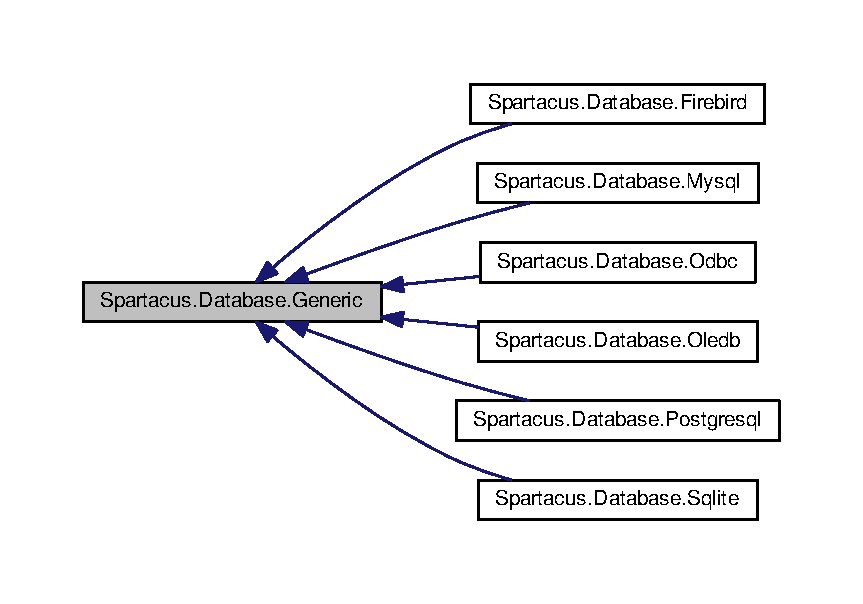
\includegraphics[width=350pt]{classSpartacus_1_1Database_1_1Generic__inherit__graph}
\end{center}
\end{figure}
\subsection*{Métodos Públicos}
\begin{DoxyCompactItemize}
\item 
\hyperlink{classSpartacus_1_1Database_1_1Generic_a622b197eddc5c95c47c848a5820addca}{Generic} (string p\+\_\+host, string p\+\_\+port, string p\+\_\+service, string p\+\_\+user, string p\+\_\+password)
\begin{DoxyCompactList}\small\item\em Inicializa uma nova instância da classe \hyperlink{classSpartacus_1_1Database_1_1Generic}{Spartacus.\+Database.\+Generic}. Armazena informações de conexão que são genéricas a qualquer S\+G\+B\+D. \end{DoxyCompactList}\item 
\hyperlink{classSpartacus_1_1Database_1_1Generic_ae767e531163e6d35c9da13bf1a26da5b}{Generic} (string p\+\_\+dsn, string p\+\_\+user, string p\+\_\+password)
\begin{DoxyCompactList}\small\item\em Inicializa uma nova instância da classe \hyperlink{classSpartacus_1_1Database_1_1Generic}{Spartacus.\+Database.\+Generic}. Armazena informações de conexão que são genéricas a qualquer S\+G\+B\+D. \end{DoxyCompactList}\item 
\hyperlink{classSpartacus_1_1Database_1_1Generic_a135fa36ed3379d3e7360a44935d3507e}{Generic} (string p\+\_\+file)
\begin{DoxyCompactList}\small\item\em Inicializa uma nova instância da classe \hyperlink{classSpartacus_1_1Database_1_1Generic}{Spartacus.\+Database.\+Generic}. Armazena informações de conexão que são genéricas a qualquer S\+G\+B\+D. \end{DoxyCompactList}\item 
abstract System.\+Data.\+Data\+Table \hyperlink{classSpartacus_1_1Database_1_1Generic_a23dc0eb8f4722d1adb1935044bc878ff}{Query} (string p\+\_\+sql, string p\+\_\+tablename)
\begin{DoxyCompactList}\small\item\em Realiza uma consulta no banco de dados, armazenando os dados de retorno em um . \end{DoxyCompactList}\item 
abstract System.\+Data.\+Data\+Table \hyperlink{classSpartacus_1_1Database_1_1Generic_a434ce0b27dfa73d909bc79c0b8471e54}{Query} (string p\+\_\+sql, string p\+\_\+tablename, System.\+Data.\+Data\+Table p\+\_\+table)
\begin{DoxyCompactList}\small\item\em Realiza uma consulta no banco de dados, armazenando os dados de retorno em um . \end{DoxyCompactList}\item 
abstract void \hyperlink{classSpartacus_1_1Database_1_1Generic_a28f1c8821906653eb4ff1484de893d16}{Execute} (string p\+\_\+sql)
\begin{DoxyCompactList}\small\item\em Executa uma instrução S\+Q\+L no banco de dados. \end{DoxyCompactList}\item 
abstract string \hyperlink{classSpartacus_1_1Database_1_1Generic_a983620fd71f520deb71ae55304b98bf6}{Execute\+Scalar} (string p\+\_\+sql)
\begin{DoxyCompactList}\small\item\em Realiza uma consulta no banco de dados, armazenando um único dado de retorno em uma string. \end{DoxyCompactList}\end{DoxyCompactItemize}
\subsection*{Campos de Dados}
\begin{DoxyCompactItemize}
\item 
string \hyperlink{classSpartacus_1_1Database_1_1Generic_adcf095a019d81c98b5f4c23ffe010cc4}{v\+\_\+host}
\begin{DoxyCompactList}\small\item\em Hostname ou I\+P onde o banco de dados está localizado. \end{DoxyCompactList}\item 
string \hyperlink{classSpartacus_1_1Database_1_1Generic_a5df6e2c77be89b3e34903ca4fc0068d0}{v\+\_\+port}
\begin{DoxyCompactList}\small\item\em Porta T\+C\+P para conectar-\/se ao S\+G\+B\+G. \end{DoxyCompactList}\item 
string \hyperlink{classSpartacus_1_1Database_1_1Generic_a3b7fd3196d76de6475c4a18edbfeea8f}{v\+\_\+service}
\begin{DoxyCompactList}\small\item\em Nome do serviço que representa o banco ao qual desejamos nos conectar. \end{DoxyCompactList}\item 
string \hyperlink{classSpartacus_1_1Database_1_1Generic_a945755698e1b479f3e581ea918338ef5}{v\+\_\+user}
\begin{DoxyCompactList}\small\item\em Usuário ou schema para se conectar ao banco de dados. \end{DoxyCompactList}\item 
string \hyperlink{classSpartacus_1_1Database_1_1Generic_a7a40ef878e5d8371034ced66a7b7b2bb}{v\+\_\+password}
\begin{DoxyCompactList}\small\item\em A senha do usuário ou schema. \end{DoxyCompactList}\item 
string \hyperlink{classSpartacus_1_1Database_1_1Generic_a91f7c26ea6ab2875fbeafc42905b423f}{v\+\_\+dsn}
\begin{DoxyCompactList}\small\item\em D\+S\+N (Data Source Name) \end{DoxyCompactList}\item 
string \hyperlink{classSpartacus_1_1Database_1_1Generic_a2afdda7bc7ad1bad84a5dc08bf6bd4e6}{v\+\_\+file}
\begin{DoxyCompactList}\small\item\em Arquivo do banco de dados. \end{DoxyCompactList}\end{DoxyCompactItemize}


\subsection{Descrição Detalhada}
Classe abstrata \hyperlink{classSpartacus_1_1Database_1_1Generic}{Spartacus.\+Database.\+Generic}. Armazena informações de conexão que são genéricas a qualquer S\+G\+B\+D. Provê polimorfismo, por ser uma classe abstrata. 



\subsection{Construtores \& Destrutores}
\hypertarget{classSpartacus_1_1Database_1_1Generic_a622b197eddc5c95c47c848a5820addca}{\index{Spartacus\+::\+Database\+::\+Generic@{Spartacus\+::\+Database\+::\+Generic}!Generic@{Generic}}
\index{Generic@{Generic}!Spartacus\+::\+Database\+::\+Generic@{Spartacus\+::\+Database\+::\+Generic}}
\subsubsection[{Generic}]{\setlength{\rightskip}{0pt plus 5cm}Spartacus.\+Database.\+Generic.\+Generic (
\begin{DoxyParamCaption}
\item[{string}]{p\+\_\+host, }
\item[{string}]{p\+\_\+port, }
\item[{string}]{p\+\_\+service, }
\item[{string}]{p\+\_\+user, }
\item[{string}]{p\+\_\+password}
\end{DoxyParamCaption}
)\hspace{0.3cm}{\ttfamily [inline]}}}\label{classSpartacus_1_1Database_1_1Generic_a622b197eddc5c95c47c848a5820addca}


Inicializa uma nova instância da classe \hyperlink{classSpartacus_1_1Database_1_1Generic}{Spartacus.\+Database.\+Generic}. Armazena informações de conexão que são genéricas a qualquer S\+G\+B\+D. 


\begin{DoxyParams}{Parâmetros}
{\em p\+\_\+host} & Hostname ou I\+P onde o banco de dados está localizado. \\
\hline
{\em p\+\_\+port} & Porta T\+C\+P para conectar-\/se ao S\+G\+B\+G. \\
\hline
{\em p\+\_\+service} & Nome do serviço que representa o banco ao qual desejamos nos conectar. \\
\hline
{\em p\+\_\+user} & Usuário ou schema para se conectar ao banco de dados. \\
\hline
{\em p\+\_\+password} & A senha do usuário ou schema. \\
\hline
\end{DoxyParams}
\hypertarget{classSpartacus_1_1Database_1_1Generic_ae767e531163e6d35c9da13bf1a26da5b}{\index{Spartacus\+::\+Database\+::\+Generic@{Spartacus\+::\+Database\+::\+Generic}!Generic@{Generic}}
\index{Generic@{Generic}!Spartacus\+::\+Database\+::\+Generic@{Spartacus\+::\+Database\+::\+Generic}}
\subsubsection[{Generic}]{\setlength{\rightskip}{0pt plus 5cm}Spartacus.\+Database.\+Generic.\+Generic (
\begin{DoxyParamCaption}
\item[{string}]{p\+\_\+dsn, }
\item[{string}]{p\+\_\+user, }
\item[{string}]{p\+\_\+password}
\end{DoxyParamCaption}
)\hspace{0.3cm}{\ttfamily [inline]}}}\label{classSpartacus_1_1Database_1_1Generic_ae767e531163e6d35c9da13bf1a26da5b}


Inicializa uma nova instância da classe \hyperlink{classSpartacus_1_1Database_1_1Generic}{Spartacus.\+Database.\+Generic}. Armazena informações de conexão que são genéricas a qualquer S\+G\+B\+D. 


\begin{DoxyParams}{Parâmetros}
{\em p\+\_\+file} & D\+S\+N (Data Source Name). \\
\hline
{\em p\+\_\+user} & Usuário ou schema para se conectar ao banco de dados. \\
\hline
{\em p\+\_\+password} & A senha do usuário ou schema. \\
\hline
\end{DoxyParams}
\hypertarget{classSpartacus_1_1Database_1_1Generic_a135fa36ed3379d3e7360a44935d3507e}{\index{Spartacus\+::\+Database\+::\+Generic@{Spartacus\+::\+Database\+::\+Generic}!Generic@{Generic}}
\index{Generic@{Generic}!Spartacus\+::\+Database\+::\+Generic@{Spartacus\+::\+Database\+::\+Generic}}
\subsubsection[{Generic}]{\setlength{\rightskip}{0pt plus 5cm}Spartacus.\+Database.\+Generic.\+Generic (
\begin{DoxyParamCaption}
\item[{string}]{p\+\_\+file}
\end{DoxyParamCaption}
)\hspace{0.3cm}{\ttfamily [inline]}}}\label{classSpartacus_1_1Database_1_1Generic_a135fa36ed3379d3e7360a44935d3507e}


Inicializa uma nova instância da classe \hyperlink{classSpartacus_1_1Database_1_1Generic}{Spartacus.\+Database.\+Generic}. Armazena informações de conexão que são genéricas a qualquer S\+G\+B\+D. 


\begin{DoxyParams}{Parâmetros}
{\em p\+\_\+file} & Arquivo do banco de dados. \\
\hline
\end{DoxyParams}


\subsection{Métodos}
\hypertarget{classSpartacus_1_1Database_1_1Generic_a28f1c8821906653eb4ff1484de893d16}{\index{Spartacus\+::\+Database\+::\+Generic@{Spartacus\+::\+Database\+::\+Generic}!Execute@{Execute}}
\index{Execute@{Execute}!Spartacus\+::\+Database\+::\+Generic@{Spartacus\+::\+Database\+::\+Generic}}
\subsubsection[{Execute}]{\setlength{\rightskip}{0pt plus 5cm}abstract void Spartacus.\+Database.\+Generic.\+Execute (
\begin{DoxyParamCaption}
\item[{string}]{p\+\_\+sql}
\end{DoxyParamCaption}
)\hspace{0.3cm}{\ttfamily [pure virtual]}}}\label{classSpartacus_1_1Database_1_1Generic_a28f1c8821906653eb4ff1484de893d16}


Executa uma instrução S\+Q\+L no banco de dados. 


\begin{DoxyParams}{Parâmetros}
{\em p\+\_\+sql} & Código S\+Q\+L a ser executado no banco de dados. \\
\hline
\end{DoxyParams}


Implementado por \hyperlink{classSpartacus_1_1Database_1_1Oledb_acfe60cb51ca949f93a1197c3cdf88231}{Spartacus.\+Database.\+Oledb}, \hyperlink{classSpartacus_1_1Database_1_1Firebird_a1844a94a27db40450a91a1d415a9d456}{Spartacus.\+Database.\+Firebird}, \hyperlink{classSpartacus_1_1Database_1_1Mysql_afdef08fb8a30287e8c550798aa6b6742}{Spartacus.\+Database.\+Mysql}, \hyperlink{classSpartacus_1_1Database_1_1Postgresql_a30357f4e3fc07945f58f9bdad4843460}{Spartacus.\+Database.\+Postgresql}, \hyperlink{classSpartacus_1_1Database_1_1Odbc_a37ff1148e0cb0c03941189bf21d9b8ed}{Spartacus.\+Database.\+Odbc} e \hyperlink{classSpartacus_1_1Database_1_1Sqlite_adb68d4ddb00d814f9741ec87e88d788a}{Spartacus.\+Database.\+Sqlite}.

\hypertarget{classSpartacus_1_1Database_1_1Generic_a983620fd71f520deb71ae55304b98bf6}{\index{Spartacus\+::\+Database\+::\+Generic@{Spartacus\+::\+Database\+::\+Generic}!Execute\+Scalar@{Execute\+Scalar}}
\index{Execute\+Scalar@{Execute\+Scalar}!Spartacus\+::\+Database\+::\+Generic@{Spartacus\+::\+Database\+::\+Generic}}
\subsubsection[{Execute\+Scalar}]{\setlength{\rightskip}{0pt plus 5cm}abstract string Spartacus.\+Database.\+Generic.\+Execute\+Scalar (
\begin{DoxyParamCaption}
\item[{string}]{p\+\_\+sql}
\end{DoxyParamCaption}
)\hspace{0.3cm}{\ttfamily [pure virtual]}}}\label{classSpartacus_1_1Database_1_1Generic_a983620fd71f520deb71ae55304b98bf6}


Realiza uma consulta no banco de dados, armazenando um único dado de retorno em uma string. 

\begin{DoxyReturn}{Retorna}
string com o dado de retorno. 
\end{DoxyReturn}

\begin{DoxyParams}{Parâmetros}
{\em p\+\_\+sql} & Código S\+Q\+L a ser consultado no banco de dados. \\
\hline
\end{DoxyParams}


Implementado por \hyperlink{classSpartacus_1_1Database_1_1Oledb_a7131081aa9dcb742321104b3a2c0c1f5}{Spartacus.\+Database.\+Oledb}, \hyperlink{classSpartacus_1_1Database_1_1Firebird_ab785abbc3e5f8b989c10c3a771981a83}{Spartacus.\+Database.\+Firebird}, \hyperlink{classSpartacus_1_1Database_1_1Mysql_ac6d8b14aed570a1a740481a0720620ab}{Spartacus.\+Database.\+Mysql}, \hyperlink{classSpartacus_1_1Database_1_1Postgresql_a4c0c196e35ba1253d5b5783c26c93d08}{Spartacus.\+Database.\+Postgresql}, \hyperlink{classSpartacus_1_1Database_1_1Odbc_ab4fcfd110084f00e66aded3478f13aca}{Spartacus.\+Database.\+Odbc} e \hyperlink{classSpartacus_1_1Database_1_1Sqlite_a0f8931cb84b7c91dce7bd45089896d46}{Spartacus.\+Database.\+Sqlite}.

\hypertarget{classSpartacus_1_1Database_1_1Generic_a23dc0eb8f4722d1adb1935044bc878ff}{\index{Spartacus\+::\+Database\+::\+Generic@{Spartacus\+::\+Database\+::\+Generic}!Query@{Query}}
\index{Query@{Query}!Spartacus\+::\+Database\+::\+Generic@{Spartacus\+::\+Database\+::\+Generic}}
\subsubsection[{Query}]{\setlength{\rightskip}{0pt plus 5cm}abstract System.\+Data.\+Data\+Table Spartacus.\+Database.\+Generic.\+Query (
\begin{DoxyParamCaption}
\item[{string}]{p\+\_\+sql, }
\item[{string}]{p\+\_\+tablename}
\end{DoxyParamCaption}
)\hspace{0.3cm}{\ttfamily [pure virtual]}}}\label{classSpartacus_1_1Database_1_1Generic_a23dc0eb8f4722d1adb1935044bc878ff}


Realiza uma consulta no banco de dados, armazenando os dados de retorno em um . 


\begin{DoxyParams}{Parâmetros}
{\em p\+\_\+sql} & Código S\+Q\+L a ser consultado no banco de dados. \\
\hline
{\em p\+\_\+tablename} & Nome virtual da tabela onde deve ser armazenado o resultado, para fins de cache. \\
\hline
\end{DoxyParams}


Implementado por \hyperlink{classSpartacus_1_1Database_1_1Oledb_a6f914652553778f6e0a683ac92ab1f87}{Spartacus.\+Database.\+Oledb}, \hyperlink{classSpartacus_1_1Database_1_1Firebird_a10235140b612dd5b178169461962d2df}{Spartacus.\+Database.\+Firebird}, \hyperlink{classSpartacus_1_1Database_1_1Mysql_a3546716a22fd53251603f2ab36d34410}{Spartacus.\+Database.\+Mysql}, \hyperlink{classSpartacus_1_1Database_1_1Postgresql_a4a60b1e3851bb0b9bec5ad3d8b6bdc4e}{Spartacus.\+Database.\+Postgresql}, \hyperlink{classSpartacus_1_1Database_1_1Odbc_a2332e648d04783ce92a9680f6cd69411}{Spartacus.\+Database.\+Odbc} e \hyperlink{classSpartacus_1_1Database_1_1Sqlite_a6b452dd40baf4fb82f3cf1dc2b5adef2}{Spartacus.\+Database.\+Sqlite}.

\hypertarget{classSpartacus_1_1Database_1_1Generic_a434ce0b27dfa73d909bc79c0b8471e54}{\index{Spartacus\+::\+Database\+::\+Generic@{Spartacus\+::\+Database\+::\+Generic}!Query@{Query}}
\index{Query@{Query}!Spartacus\+::\+Database\+::\+Generic@{Spartacus\+::\+Database\+::\+Generic}}
\subsubsection[{Query}]{\setlength{\rightskip}{0pt plus 5cm}abstract System.\+Data.\+Data\+Table Spartacus.\+Database.\+Generic.\+Query (
\begin{DoxyParamCaption}
\item[{string}]{p\+\_\+sql, }
\item[{string}]{p\+\_\+tablename, }
\item[{System.\+Data.\+Data\+Table}]{p\+\_\+table}
\end{DoxyParamCaption}
)\hspace{0.3cm}{\ttfamily [pure virtual]}}}\label{classSpartacus_1_1Database_1_1Generic_a434ce0b27dfa73d909bc79c0b8471e54}


Realiza uma consulta no banco de dados, armazenando os dados de retorno em um . 


\begin{DoxyParams}{Parâmetros}
{\em p\+\_\+sql} & Código S\+Q\+L a ser consultado no banco de dados. \\
\hline
{\em p\+\_\+tablename} & Nome virtual da tabela onde deve ser armazenado o resultado, para fins de cache. \\
\hline
{\em p\+\_\+table} & Tabela que contém definições de nomes e tipos de colunas. \\
\hline
\end{DoxyParams}


Implementado por \hyperlink{classSpartacus_1_1Database_1_1Oledb_ab5f3ae20ac53dcc95182c0845a04d460}{Spartacus.\+Database.\+Oledb}, \hyperlink{classSpartacus_1_1Database_1_1Firebird_a6243d18345e2b5f44ddcda032f6b2b9e}{Spartacus.\+Database.\+Firebird}, \hyperlink{classSpartacus_1_1Database_1_1Mysql_a2b7f2096a3ee819670c49ed41cf04f75}{Spartacus.\+Database.\+Mysql}, \hyperlink{classSpartacus_1_1Database_1_1Postgresql_ad14dbb0c81571d02b368388d8a8ebd97}{Spartacus.\+Database.\+Postgresql}, \hyperlink{classSpartacus_1_1Database_1_1Odbc_a7b6d07dad45f3124d081976d2b51ed4b}{Spartacus.\+Database.\+Odbc} e \hyperlink{classSpartacus_1_1Database_1_1Sqlite_a935c96905011800e4df8ad0a7ca9bcf3}{Spartacus.\+Database.\+Sqlite}.



\subsection{Campos}
\hypertarget{classSpartacus_1_1Database_1_1Generic_a91f7c26ea6ab2875fbeafc42905b423f}{\index{Spartacus\+::\+Database\+::\+Generic@{Spartacus\+::\+Database\+::\+Generic}!v\+\_\+dsn@{v\+\_\+dsn}}
\index{v\+\_\+dsn@{v\+\_\+dsn}!Spartacus\+::\+Database\+::\+Generic@{Spartacus\+::\+Database\+::\+Generic}}
\subsubsection[{v\+\_\+dsn}]{\setlength{\rightskip}{0pt plus 5cm}string Spartacus.\+Database.\+Generic.\+v\+\_\+dsn}}\label{classSpartacus_1_1Database_1_1Generic_a91f7c26ea6ab2875fbeafc42905b423f}


D\+S\+N (Data Source Name) 

\hypertarget{classSpartacus_1_1Database_1_1Generic_a2afdda7bc7ad1bad84a5dc08bf6bd4e6}{\index{Spartacus\+::\+Database\+::\+Generic@{Spartacus\+::\+Database\+::\+Generic}!v\+\_\+file@{v\+\_\+file}}
\index{v\+\_\+file@{v\+\_\+file}!Spartacus\+::\+Database\+::\+Generic@{Spartacus\+::\+Database\+::\+Generic}}
\subsubsection[{v\+\_\+file}]{\setlength{\rightskip}{0pt plus 5cm}string Spartacus.\+Database.\+Generic.\+v\+\_\+file}}\label{classSpartacus_1_1Database_1_1Generic_a2afdda7bc7ad1bad84a5dc08bf6bd4e6}


Arquivo do banco de dados. 

\hypertarget{classSpartacus_1_1Database_1_1Generic_adcf095a019d81c98b5f4c23ffe010cc4}{\index{Spartacus\+::\+Database\+::\+Generic@{Spartacus\+::\+Database\+::\+Generic}!v\+\_\+host@{v\+\_\+host}}
\index{v\+\_\+host@{v\+\_\+host}!Spartacus\+::\+Database\+::\+Generic@{Spartacus\+::\+Database\+::\+Generic}}
\subsubsection[{v\+\_\+host}]{\setlength{\rightskip}{0pt plus 5cm}string Spartacus.\+Database.\+Generic.\+v\+\_\+host}}\label{classSpartacus_1_1Database_1_1Generic_adcf095a019d81c98b5f4c23ffe010cc4}


Hostname ou I\+P onde o banco de dados está localizado. 

\hypertarget{classSpartacus_1_1Database_1_1Generic_a7a40ef878e5d8371034ced66a7b7b2bb}{\index{Spartacus\+::\+Database\+::\+Generic@{Spartacus\+::\+Database\+::\+Generic}!v\+\_\+password@{v\+\_\+password}}
\index{v\+\_\+password@{v\+\_\+password}!Spartacus\+::\+Database\+::\+Generic@{Spartacus\+::\+Database\+::\+Generic}}
\subsubsection[{v\+\_\+password}]{\setlength{\rightskip}{0pt plus 5cm}string Spartacus.\+Database.\+Generic.\+v\+\_\+password}}\label{classSpartacus_1_1Database_1_1Generic_a7a40ef878e5d8371034ced66a7b7b2bb}


A senha do usuário ou schema. 

\hypertarget{classSpartacus_1_1Database_1_1Generic_a5df6e2c77be89b3e34903ca4fc0068d0}{\index{Spartacus\+::\+Database\+::\+Generic@{Spartacus\+::\+Database\+::\+Generic}!v\+\_\+port@{v\+\_\+port}}
\index{v\+\_\+port@{v\+\_\+port}!Spartacus\+::\+Database\+::\+Generic@{Spartacus\+::\+Database\+::\+Generic}}
\subsubsection[{v\+\_\+port}]{\setlength{\rightskip}{0pt plus 5cm}string Spartacus.\+Database.\+Generic.\+v\+\_\+port}}\label{classSpartacus_1_1Database_1_1Generic_a5df6e2c77be89b3e34903ca4fc0068d0}


Porta T\+C\+P para conectar-\/se ao S\+G\+B\+G. 

\hypertarget{classSpartacus_1_1Database_1_1Generic_a3b7fd3196d76de6475c4a18edbfeea8f}{\index{Spartacus\+::\+Database\+::\+Generic@{Spartacus\+::\+Database\+::\+Generic}!v\+\_\+service@{v\+\_\+service}}
\index{v\+\_\+service@{v\+\_\+service}!Spartacus\+::\+Database\+::\+Generic@{Spartacus\+::\+Database\+::\+Generic}}
\subsubsection[{v\+\_\+service}]{\setlength{\rightskip}{0pt plus 5cm}string Spartacus.\+Database.\+Generic.\+v\+\_\+service}}\label{classSpartacus_1_1Database_1_1Generic_a3b7fd3196d76de6475c4a18edbfeea8f}


Nome do serviço que representa o banco ao qual desejamos nos conectar. 

\hypertarget{classSpartacus_1_1Database_1_1Generic_a945755698e1b479f3e581ea918338ef5}{\index{Spartacus\+::\+Database\+::\+Generic@{Spartacus\+::\+Database\+::\+Generic}!v\+\_\+user@{v\+\_\+user}}
\index{v\+\_\+user@{v\+\_\+user}!Spartacus\+::\+Database\+::\+Generic@{Spartacus\+::\+Database\+::\+Generic}}
\subsubsection[{v\+\_\+user}]{\setlength{\rightskip}{0pt plus 5cm}string Spartacus.\+Database.\+Generic.\+v\+\_\+user}}\label{classSpartacus_1_1Database_1_1Generic_a945755698e1b479f3e581ea918338ef5}


Usuário ou schema para se conectar ao banco de dados. 



A documentação para esta classe foi gerada a partir do seguinte arquivo\+:\begin{DoxyCompactItemize}
\item 
Spartacus.\+Database.\+Generic.\+cs\end{DoxyCompactItemize}

\hypertarget{classSpartacus_1_1Database_1_1Mysql}{\section{Referência da Classe Spartacus.\+Database.\+Mysql}
\label{classSpartacus_1_1Database_1_1Mysql}\index{Spartacus.\+Database.\+Mysql@{Spartacus.\+Database.\+Mysql}}
}


Classe \hyperlink{classSpartacus_1_1Database_1_1Mysql}{Spartacus.\+Database.\+Mysql}. Herda da classe \hyperlink{classSpartacus_1_1Database_1_1Generic}{Spartacus.\+Database.\+Generic}. Utiliza o My\+S\+Q\+L .N\+E\+T Provider para acessar um S\+G\+B\+D My\+S\+Q\+L.  




Diagrama de Hierarquia para Spartacus.\+Database.\+Mysql\+:


Diagrama de colaboração para Spartacus.\+Database.\+Mysql\+:
\subsection*{Métodos Públicos}
\begin{DoxyCompactItemize}
\item 
\hyperlink{classSpartacus_1_1Database_1_1Mysql_aa1a7b4639cb22e84da677a4186efa060}{Mysql} (string p\+\_\+server, string p\+\_\+port, string p\+\_\+database, string p\+\_\+user, string p\+\_\+password)
\begin{DoxyCompactList}\small\item\em Inicializa uma nova instancia da classe \hyperlink{classSpartacus_1_1Database_1_1Mysql}{Spartacus.\+Database.\+Mysql}. \end{DoxyCompactList}\item 
override void \hyperlink{classSpartacus_1_1Database_1_1Mysql_a5169783f95c51db388b841b4bd9207f5}{Connect} ()
\begin{DoxyCompactList}\small\item\em Conectar ao banco de dados. \end{DoxyCompactList}\item 
override void \hyperlink{classSpartacus_1_1Database_1_1Mysql_ab7000e1b5ceedaaeaf3c824e22ec1b14}{Disconnect} ()
\begin{DoxyCompactList}\small\item\em Desconectar do banco de dados. \end{DoxyCompactList}\item 
override System.\+Data.\+Data\+Table \hyperlink{classSpartacus_1_1Database_1_1Mysql_a3546716a22fd53251603f2ab36d34410}{Query} (string p\+\_\+sql, string p\+\_\+tablename)
\begin{DoxyCompactList}\small\item\em Realiza uma consulta no banco de dados, armazenando os dados de retorno em um System.\+Data.\+Data\+Table. \end{DoxyCompactList}\item 
override System.\+Data.\+Data\+Table \hyperlink{classSpartacus_1_1Database_1_1Mysql_a2b7f2096a3ee819670c49ed41cf04f75}{Query} (string p\+\_\+sql, string p\+\_\+tablename, System.\+Data.\+Data\+Table p\+\_\+table)
\begin{DoxyCompactList}\small\item\em Realiza uma consulta no banco de dados, armazenando os dados de retorno em um System.\+Data.\+Data\+Table. \end{DoxyCompactList}\item 
override void \hyperlink{classSpartacus_1_1Database_1_1Mysql_afdef08fb8a30287e8c550798aa6b6742}{Execute} (string p\+\_\+sql)
\begin{DoxyCompactList}\small\item\em Executa um código S\+Q\+L no banco de dados. \end{DoxyCompactList}\item 
override string \hyperlink{classSpartacus_1_1Database_1_1Mysql_ac6d8b14aed570a1a740481a0720620ab}{Execute\+Scalar} (string p\+\_\+sql)
\begin{DoxyCompactList}\small\item\em Realiza uma consulta no banco de dados, armazenando um único dado de retorno em uma string. \end{DoxyCompactList}\end{DoxyCompactItemize}
\subsection*{Campos de Dados}
\begin{DoxyCompactItemize}
\item 
string \hyperlink{classSpartacus_1_1Database_1_1Mysql_ac29f25cd328e6bedd0b2f122040674ca}{v\+\_\+connectionstring}
\begin{DoxyCompactList}\small\item\em String de conexão para acessar o banco. \end{DoxyCompactList}\end{DoxyCompactItemize}


\subsection{Descrição Detalhada}
Classe \hyperlink{classSpartacus_1_1Database_1_1Mysql}{Spartacus.\+Database.\+Mysql}. Herda da classe \hyperlink{classSpartacus_1_1Database_1_1Generic}{Spartacus.\+Database.\+Generic}. Utiliza o My\+S\+Q\+L .N\+E\+T Provider para acessar um S\+G\+B\+D My\+S\+Q\+L. 



\subsection{Construtores \& Destrutores}
\hypertarget{classSpartacus_1_1Database_1_1Mysql_aa1a7b4639cb22e84da677a4186efa060}{\index{Spartacus\+::\+Database\+::\+Mysql@{Spartacus\+::\+Database\+::\+Mysql}!Mysql@{Mysql}}
\index{Mysql@{Mysql}!Spartacus\+::\+Database\+::\+Mysql@{Spartacus\+::\+Database\+::\+Mysql}}
\subsubsection[{Mysql}]{\setlength{\rightskip}{0pt plus 5cm}Spartacus.\+Database.\+Mysql.\+Mysql (
\begin{DoxyParamCaption}
\item[{string}]{p\+\_\+server, }
\item[{string}]{p\+\_\+port, }
\item[{string}]{p\+\_\+database, }
\item[{string}]{p\+\_\+user, }
\item[{string}]{p\+\_\+password}
\end{DoxyParamCaption}
)\hspace{0.3cm}{\ttfamily [inline]}}}\label{classSpartacus_1_1Database_1_1Mysql_aa1a7b4639cb22e84da677a4186efa060}


Inicializa uma nova instancia da classe \hyperlink{classSpartacus_1_1Database_1_1Mysql}{Spartacus.\+Database.\+Mysql}. 


\begin{DoxyParams}{Parâmetros}
{\em p\+\_\+server} & I\+P do servidor My\+S\+Q\+L. \\
\hline
{\em p\+\_\+port} & Porta de conexão. \\
\hline
{\em p\+\_\+database} & Nome da base de dados ou schema. \\
\hline
{\em p\+\_\+user} & Usuário do My\+S\+Q\+L. \\
\hline
{\em p\+\_\+password} & Senha do My\+S\+Q\+L. \\
\hline
\end{DoxyParams}


\subsection{Métodos}
\hypertarget{classSpartacus_1_1Database_1_1Mysql_a5169783f95c51db388b841b4bd9207f5}{\index{Spartacus\+::\+Database\+::\+Mysql@{Spartacus\+::\+Database\+::\+Mysql}!Connect@{Connect}}
\index{Connect@{Connect}!Spartacus\+::\+Database\+::\+Mysql@{Spartacus\+::\+Database\+::\+Mysql}}
\subsubsection[{Connect}]{\setlength{\rightskip}{0pt plus 5cm}override void Spartacus.\+Database.\+Mysql.\+Connect (
\begin{DoxyParamCaption}
{}
\end{DoxyParamCaption}
)\hspace{0.3cm}{\ttfamily [inline]}, {\ttfamily [virtual]}}}\label{classSpartacus_1_1Database_1_1Mysql_a5169783f95c51db388b841b4bd9207f5}


Conectar ao banco de dados. 


\begin{DoxyExceptions}{Exceções}
{\em \hyperlink{classSpartacus_1_1Database_1_1Exception}{Spartacus.\+Database.\+Exception}} & Exceção acontece quando não for possível se conectar ao banco de dados.\\
\hline
\end{DoxyExceptions}


Implementa \hyperlink{classSpartacus_1_1Database_1_1Generic_a0f3940aeabde41676f15366e83eff166}{Spartacus.\+Database.\+Generic}.

\hypertarget{classSpartacus_1_1Database_1_1Mysql_ab7000e1b5ceedaaeaf3c824e22ec1b14}{\index{Spartacus\+::\+Database\+::\+Mysql@{Spartacus\+::\+Database\+::\+Mysql}!Disconnect@{Disconnect}}
\index{Disconnect@{Disconnect}!Spartacus\+::\+Database\+::\+Mysql@{Spartacus\+::\+Database\+::\+Mysql}}
\subsubsection[{Disconnect}]{\setlength{\rightskip}{0pt plus 5cm}override void Spartacus.\+Database.\+Mysql.\+Disconnect (
\begin{DoxyParamCaption}
{}
\end{DoxyParamCaption}
)\hspace{0.3cm}{\ttfamily [inline]}, {\ttfamily [virtual]}}}\label{classSpartacus_1_1Database_1_1Mysql_ab7000e1b5ceedaaeaf3c824e22ec1b14}


Desconectar do banco de dados. 


\begin{DoxyExceptions}{Exceções}
{\em \hyperlink{classSpartacus_1_1Database_1_1Exception}{Spartacus.\+Database.\+Exception}} & Exceção acontece quando não for possível se desconectar do banco de dados.\\
\hline
\end{DoxyExceptions}


Implementa \hyperlink{classSpartacus_1_1Database_1_1Generic_a765dda5d5d8a768885fabd9799a0a180}{Spartacus.\+Database.\+Generic}.

\hypertarget{classSpartacus_1_1Database_1_1Mysql_afdef08fb8a30287e8c550798aa6b6742}{\index{Spartacus\+::\+Database\+::\+Mysql@{Spartacus\+::\+Database\+::\+Mysql}!Execute@{Execute}}
\index{Execute@{Execute}!Spartacus\+::\+Database\+::\+Mysql@{Spartacus\+::\+Database\+::\+Mysql}}
\subsubsection[{Execute}]{\setlength{\rightskip}{0pt plus 5cm}override void Spartacus.\+Database.\+Mysql.\+Execute (
\begin{DoxyParamCaption}
\item[{string}]{p\+\_\+sql}
\end{DoxyParamCaption}
)\hspace{0.3cm}{\ttfamily [inline]}, {\ttfamily [virtual]}}}\label{classSpartacus_1_1Database_1_1Mysql_afdef08fb8a30287e8c550798aa6b6742}


Executa um código S\+Q\+L no banco de dados. 


\begin{DoxyParams}{Parâmetros}
{\em p\+\_\+sql} & Código S\+Q\+L a ser executado no banco de dados. \\
\hline
\end{DoxyParams}

\begin{DoxyExceptions}{Exceções}
{\em \hyperlink{classSpartacus_1_1Database_1_1Exception}{Spartacus.\+Database.\+Exception}} & Exceção acontece quando não for possível executar o código S\+Q\+L.\\
\hline
\end{DoxyExceptions}


Implementa \hyperlink{classSpartacus_1_1Database_1_1Generic_a28f1c8821906653eb4ff1484de893d16}{Spartacus.\+Database.\+Generic}.

\hypertarget{classSpartacus_1_1Database_1_1Mysql_ac6d8b14aed570a1a740481a0720620ab}{\index{Spartacus\+::\+Database\+::\+Mysql@{Spartacus\+::\+Database\+::\+Mysql}!Execute\+Scalar@{Execute\+Scalar}}
\index{Execute\+Scalar@{Execute\+Scalar}!Spartacus\+::\+Database\+::\+Mysql@{Spartacus\+::\+Database\+::\+Mysql}}
\subsubsection[{Execute\+Scalar}]{\setlength{\rightskip}{0pt plus 5cm}override string Spartacus.\+Database.\+Mysql.\+Execute\+Scalar (
\begin{DoxyParamCaption}
\item[{string}]{p\+\_\+sql}
\end{DoxyParamCaption}
)\hspace{0.3cm}{\ttfamily [inline]}, {\ttfamily [virtual]}}}\label{classSpartacus_1_1Database_1_1Mysql_ac6d8b14aed570a1a740481a0720620ab}


Realiza uma consulta no banco de dados, armazenando um único dado de retorno em uma string. 

\begin{DoxyReturn}{Retorna}
string com o dado de retorno. 
\end{DoxyReturn}

\begin{DoxyParams}{Parâmetros}
{\em p\+\_\+sql} & Código S\+Q\+L a ser consultado no banco de dados. \\
\hline
\end{DoxyParams}

\begin{DoxyExceptions}{Exceções}
{\em \hyperlink{classSpartacus_1_1Database_1_1Exception}{Spartacus.\+Database.\+Exception}} & Exceção acontece quando não for possível executar o código S\+Q\+L.\\
\hline
\end{DoxyExceptions}


Implementa \hyperlink{classSpartacus_1_1Database_1_1Generic_a983620fd71f520deb71ae55304b98bf6}{Spartacus.\+Database.\+Generic}.

\hypertarget{classSpartacus_1_1Database_1_1Mysql_a3546716a22fd53251603f2ab36d34410}{\index{Spartacus\+::\+Database\+::\+Mysql@{Spartacus\+::\+Database\+::\+Mysql}!Query@{Query}}
\index{Query@{Query}!Spartacus\+::\+Database\+::\+Mysql@{Spartacus\+::\+Database\+::\+Mysql}}
\subsubsection[{Query}]{\setlength{\rightskip}{0pt plus 5cm}override System.\+Data.\+Data\+Table Spartacus.\+Database.\+Mysql.\+Query (
\begin{DoxyParamCaption}
\item[{string}]{p\+\_\+sql, }
\item[{string}]{p\+\_\+tablename}
\end{DoxyParamCaption}
)\hspace{0.3cm}{\ttfamily [inline]}, {\ttfamily [virtual]}}}\label{classSpartacus_1_1Database_1_1Mysql_a3546716a22fd53251603f2ab36d34410}


Realiza uma consulta no banco de dados, armazenando os dados de retorno em um System.\+Data.\+Data\+Table. 


\begin{DoxyParams}{Parâmetros}
{\em p\+\_\+sql} & Código S\+Q\+L a ser consultado no banco de dados. \\
\hline
{\em p\+\_\+tablename} & Nome virtual da tabela onde deve ser armazenado o resultado, para fins de cache. \\
\hline
\end{DoxyParams}
\begin{DoxyReturn}{Retorna}
Retorna uma System.\+Data.\+Data\+Table com os dados de retorno da consulta.
\end{DoxyReturn}

\begin{DoxyExceptions}{Exceções}
{\em \hyperlink{classSpartacus_1_1Database_1_1Exception}{Spartacus.\+Database.\+Exception}} & Exceção acontece quando não for possível executar a consulta.\\
\hline
\end{DoxyExceptions}


Implementa \hyperlink{classSpartacus_1_1Database_1_1Generic_a23dc0eb8f4722d1adb1935044bc878ff}{Spartacus.\+Database.\+Generic}.

\hypertarget{classSpartacus_1_1Database_1_1Mysql_a2b7f2096a3ee819670c49ed41cf04f75}{\index{Spartacus\+::\+Database\+::\+Mysql@{Spartacus\+::\+Database\+::\+Mysql}!Query@{Query}}
\index{Query@{Query}!Spartacus\+::\+Database\+::\+Mysql@{Spartacus\+::\+Database\+::\+Mysql}}
\subsubsection[{Query}]{\setlength{\rightskip}{0pt plus 5cm}override System.\+Data.\+Data\+Table Spartacus.\+Database.\+Mysql.\+Query (
\begin{DoxyParamCaption}
\item[{string}]{p\+\_\+sql, }
\item[{string}]{p\+\_\+tablename, }
\item[{System.\+Data.\+Data\+Table}]{p\+\_\+table}
\end{DoxyParamCaption}
)\hspace{0.3cm}{\ttfamily [inline]}, {\ttfamily [virtual]}}}\label{classSpartacus_1_1Database_1_1Mysql_a2b7f2096a3ee819670c49ed41cf04f75}


Realiza uma consulta no banco de dados, armazenando os dados de retorno em um System.\+Data.\+Data\+Table. 


\begin{DoxyParams}{Parâmetros}
{\em p\+\_\+sql} & Código S\+Q\+L a ser consultado no banco de dados. \\
\hline
{\em p\+\_\+tablename} & Nome virtual da tabela onde deve ser armazenado o resultado, para fins de cache. \\
\hline
{\em p\+\_\+table} & Tabela que contém definições de nomes e tipos de colunas. \\
\hline
\end{DoxyParams}
\begin{DoxyReturn}{Retorna}
Retorna uma System.\+Data.\+Data\+Table com os dados de retorno da consulta.
\end{DoxyReturn}

\begin{DoxyExceptions}{Exceções}
{\em \hyperlink{classSpartacus_1_1Database_1_1Exception}{Spartacus.\+Database.\+Exception}} & Exceção acontece quando não for possível executar a consulta.\\
\hline
\end{DoxyExceptions}


Implementa \hyperlink{classSpartacus_1_1Database_1_1Generic_a434ce0b27dfa73d909bc79c0b8471e54}{Spartacus.\+Database.\+Generic}.



\subsection{Campos}
\hypertarget{classSpartacus_1_1Database_1_1Mysql_ac29f25cd328e6bedd0b2f122040674ca}{\index{Spartacus\+::\+Database\+::\+Mysql@{Spartacus\+::\+Database\+::\+Mysql}!v\+\_\+connectionstring@{v\+\_\+connectionstring}}
\index{v\+\_\+connectionstring@{v\+\_\+connectionstring}!Spartacus\+::\+Database\+::\+Mysql@{Spartacus\+::\+Database\+::\+Mysql}}
\subsubsection[{v\+\_\+connectionstring}]{\setlength{\rightskip}{0pt plus 5cm}string Spartacus.\+Database.\+Mysql.\+v\+\_\+connectionstring}}\label{classSpartacus_1_1Database_1_1Mysql_ac29f25cd328e6bedd0b2f122040674ca}


String de conexão para acessar o banco. 



A documentação para esta classe foi gerada a partir do seguinte arquivo\+:\begin{DoxyCompactItemize}
\item 
Spartacus.\+Database.\+Mysql.\+cs\end{DoxyCompactItemize}

\hypertarget{classSpartacus_1_1Database_1_1Odbc}{\section{Referência da Classe Spartacus.\+Database.\+Odbc}
\label{classSpartacus_1_1Database_1_1Odbc}\index{Spartacus.\+Database.\+Odbc@{Spartacus.\+Database.\+Odbc}}
}


Classe \hyperlink{classSpartacus_1_1Database_1_1Odbc}{Spartacus.\+Database.\+Odbc}. Herda da classe \hyperlink{classSpartacus_1_1Database_1_1Generic}{Spartacus.\+Database.\+Generic}. Utiliza a implementação O\+D\+B\+C (Open \hyperlink{namespaceSpartacus_1_1Database}{Database} Connectivity) para acessar qualquer S\+G\+B\+D.  




Diagrama de Hierarquia para Spartacus.\+Database.\+Odbc\+:


Diagrama de colaboração para Spartacus.\+Database.\+Odbc\+:
\subsection*{Métodos Públicos}
\begin{DoxyCompactItemize}
\item 
\hyperlink{classSpartacus_1_1Database_1_1Odbc_a2ea31921d3a0d8e25b73a05e89784bdc}{Odbc} (string p\+\_\+dsn, string p\+\_\+user, string p\+\_\+password)
\begin{DoxyCompactList}\small\item\em Inicializa uma nova instância da classe \hyperlink{classSpartacus_1_1Database_1_1Odbc}{Spartacus.\+Database.\+Odbc}. Cria a string de conexão ao banco. \end{DoxyCompactList}\item 
override void \hyperlink{classSpartacus_1_1Database_1_1Odbc_a306058e9deb3a18bfdb228488a5d7641}{Connect} ()
\begin{DoxyCompactList}\small\item\em Conectar ao banco de dados. \end{DoxyCompactList}\item 
override void \hyperlink{classSpartacus_1_1Database_1_1Odbc_a7b2a59398269853f6ad7f3af308afadf}{Disconnect} ()
\begin{DoxyCompactList}\small\item\em Desconectar do banco de dados. \end{DoxyCompactList}\item 
override System.\+Data.\+Data\+Table \hyperlink{classSpartacus_1_1Database_1_1Odbc_a2332e648d04783ce92a9680f6cd69411}{Query} (string p\+\_\+sql, string p\+\_\+tablename)
\begin{DoxyCompactList}\small\item\em Realiza uma consulta no banco de dados, armazenando os dados de retorno em um System.\+Data.\+Data\+Table. \end{DoxyCompactList}\item 
override System.\+Data.\+Data\+Table \hyperlink{classSpartacus_1_1Database_1_1Odbc_a7b6d07dad45f3124d081976d2b51ed4b}{Query} (string p\+\_\+sql, string p\+\_\+tablename, System.\+Data.\+Data\+Table p\+\_\+table)
\begin{DoxyCompactList}\small\item\em Realiza uma consulta no banco de dados, armazenando os dados de retorno em um System.\+Data.\+Data\+Table. \end{DoxyCompactList}\item 
override void \hyperlink{classSpartacus_1_1Database_1_1Odbc_a37ff1148e0cb0c03941189bf21d9b8ed}{Execute} (string p\+\_\+sql)
\begin{DoxyCompactList}\small\item\em Executa um código S\+Q\+L no banco de dados. \end{DoxyCompactList}\item 
override string \hyperlink{classSpartacus_1_1Database_1_1Odbc_ab4fcfd110084f00e66aded3478f13aca}{Execute\+Scalar} (string p\+\_\+sql)
\begin{DoxyCompactList}\small\item\em Realiza uma consulta no banco de dados, armazenando um único dado de retorno em uma string. \end{DoxyCompactList}\end{DoxyCompactItemize}
\subsection*{Campos de Dados}
\begin{DoxyCompactItemize}
\item 
string \hyperlink{classSpartacus_1_1Database_1_1Odbc_a4f31d12ddac65ac9ce6ab02eb7fbced8}{v\+\_\+connectionstring}
\begin{DoxyCompactList}\small\item\em String de conexão para acessar o banco. \end{DoxyCompactList}\end{DoxyCompactItemize}


\subsection{Descrição Detalhada}
Classe \hyperlink{classSpartacus_1_1Database_1_1Odbc}{Spartacus.\+Database.\+Odbc}. Herda da classe \hyperlink{classSpartacus_1_1Database_1_1Generic}{Spartacus.\+Database.\+Generic}. Utiliza a implementação O\+D\+B\+C (Open \hyperlink{namespaceSpartacus_1_1Database}{Database} Connectivity) para acessar qualquer S\+G\+B\+D. 



\subsection{Construtores \& Destrutores}
\hypertarget{classSpartacus_1_1Database_1_1Odbc_a2ea31921d3a0d8e25b73a05e89784bdc}{\index{Spartacus\+::\+Database\+::\+Odbc@{Spartacus\+::\+Database\+::\+Odbc}!Odbc@{Odbc}}
\index{Odbc@{Odbc}!Spartacus\+::\+Database\+::\+Odbc@{Spartacus\+::\+Database\+::\+Odbc}}
\subsubsection[{Odbc}]{\setlength{\rightskip}{0pt plus 5cm}Spartacus.\+Database.\+Odbc.\+Odbc (
\begin{DoxyParamCaption}
\item[{string}]{p\+\_\+dsn, }
\item[{string}]{p\+\_\+user, }
\item[{string}]{p\+\_\+password}
\end{DoxyParamCaption}
)\hspace{0.3cm}{\ttfamily [inline]}}}\label{classSpartacus_1_1Database_1_1Odbc_a2ea31921d3a0d8e25b73a05e89784bdc}


Inicializa uma nova instância da classe \hyperlink{classSpartacus_1_1Database_1_1Odbc}{Spartacus.\+Database.\+Odbc}. Cria a string de conexão ao banco. 


\begin{DoxyParams}{Parâmetros}
{\em p\+\_\+dsn} & D\+S\+N (Data Source Name). \\
\hline
{\em p\+\_\+user} & Usuário ou schema para se conectar ao banco de dados. \\
\hline
{\em p\+\_\+password} & A senha do usuário ou schema. \\
\hline
\end{DoxyParams}


\subsection{Métodos}
\hypertarget{classSpartacus_1_1Database_1_1Odbc_a306058e9deb3a18bfdb228488a5d7641}{\index{Spartacus\+::\+Database\+::\+Odbc@{Spartacus\+::\+Database\+::\+Odbc}!Connect@{Connect}}
\index{Connect@{Connect}!Spartacus\+::\+Database\+::\+Odbc@{Spartacus\+::\+Database\+::\+Odbc}}
\subsubsection[{Connect}]{\setlength{\rightskip}{0pt plus 5cm}override void Spartacus.\+Database.\+Odbc.\+Connect (
\begin{DoxyParamCaption}
{}
\end{DoxyParamCaption}
)\hspace{0.3cm}{\ttfamily [inline]}, {\ttfamily [virtual]}}}\label{classSpartacus_1_1Database_1_1Odbc_a306058e9deb3a18bfdb228488a5d7641}


Conectar ao banco de dados. 


\begin{DoxyExceptions}{Exceções}
{\em \hyperlink{classSpartacus_1_1Database_1_1Exception}{Spartacus.\+Database.\+Exception}} & Exceção acontece quando não for possível se conectar ao banco de dados.\\
\hline
\end{DoxyExceptions}


Implementa \hyperlink{classSpartacus_1_1Database_1_1Generic_a0f3940aeabde41676f15366e83eff166}{Spartacus.\+Database.\+Generic}.

\hypertarget{classSpartacus_1_1Database_1_1Odbc_a7b2a59398269853f6ad7f3af308afadf}{\index{Spartacus\+::\+Database\+::\+Odbc@{Spartacus\+::\+Database\+::\+Odbc}!Disconnect@{Disconnect}}
\index{Disconnect@{Disconnect}!Spartacus\+::\+Database\+::\+Odbc@{Spartacus\+::\+Database\+::\+Odbc}}
\subsubsection[{Disconnect}]{\setlength{\rightskip}{0pt plus 5cm}override void Spartacus.\+Database.\+Odbc.\+Disconnect (
\begin{DoxyParamCaption}
{}
\end{DoxyParamCaption}
)\hspace{0.3cm}{\ttfamily [inline]}, {\ttfamily [virtual]}}}\label{classSpartacus_1_1Database_1_1Odbc_a7b2a59398269853f6ad7f3af308afadf}


Desconectar do banco de dados. 


\begin{DoxyExceptions}{Exceções}
{\em \hyperlink{classSpartacus_1_1Database_1_1Exception}{Spartacus.\+Database.\+Exception}} & Exceção acontece quando não for possível se desconectar do banco de dados.\\
\hline
\end{DoxyExceptions}


Implementa \hyperlink{classSpartacus_1_1Database_1_1Generic_a765dda5d5d8a768885fabd9799a0a180}{Spartacus.\+Database.\+Generic}.

\hypertarget{classSpartacus_1_1Database_1_1Odbc_a37ff1148e0cb0c03941189bf21d9b8ed}{\index{Spartacus\+::\+Database\+::\+Odbc@{Spartacus\+::\+Database\+::\+Odbc}!Execute@{Execute}}
\index{Execute@{Execute}!Spartacus\+::\+Database\+::\+Odbc@{Spartacus\+::\+Database\+::\+Odbc}}
\subsubsection[{Execute}]{\setlength{\rightskip}{0pt plus 5cm}override void Spartacus.\+Database.\+Odbc.\+Execute (
\begin{DoxyParamCaption}
\item[{string}]{p\+\_\+sql}
\end{DoxyParamCaption}
)\hspace{0.3cm}{\ttfamily [inline]}, {\ttfamily [virtual]}}}\label{classSpartacus_1_1Database_1_1Odbc_a37ff1148e0cb0c03941189bf21d9b8ed}


Executa um código S\+Q\+L no banco de dados. 


\begin{DoxyParams}{Parâmetros}
{\em p\+\_\+sql} & Código S\+Q\+L a ser executado no banco de dados. \\
\hline
\end{DoxyParams}

\begin{DoxyExceptions}{Exceções}
{\em \hyperlink{classSpartacus_1_1Database_1_1Exception}{Spartacus.\+Database.\+Exception}} & Exceção acontece quando não for possível executar o código S\+Q\+L.\\
\hline
\end{DoxyExceptions}


Implementa \hyperlink{classSpartacus_1_1Database_1_1Generic_a28f1c8821906653eb4ff1484de893d16}{Spartacus.\+Database.\+Generic}.

\hypertarget{classSpartacus_1_1Database_1_1Odbc_ab4fcfd110084f00e66aded3478f13aca}{\index{Spartacus\+::\+Database\+::\+Odbc@{Spartacus\+::\+Database\+::\+Odbc}!Execute\+Scalar@{Execute\+Scalar}}
\index{Execute\+Scalar@{Execute\+Scalar}!Spartacus\+::\+Database\+::\+Odbc@{Spartacus\+::\+Database\+::\+Odbc}}
\subsubsection[{Execute\+Scalar}]{\setlength{\rightskip}{0pt plus 5cm}override string Spartacus.\+Database.\+Odbc.\+Execute\+Scalar (
\begin{DoxyParamCaption}
\item[{string}]{p\+\_\+sql}
\end{DoxyParamCaption}
)\hspace{0.3cm}{\ttfamily [inline]}, {\ttfamily [virtual]}}}\label{classSpartacus_1_1Database_1_1Odbc_ab4fcfd110084f00e66aded3478f13aca}


Realiza uma consulta no banco de dados, armazenando um único dado de retorno em uma string. 

\begin{DoxyReturn}{Retorna}
string com o dado de retorno. 
\end{DoxyReturn}

\begin{DoxyParams}{Parâmetros}
{\em p\+\_\+sql} & Código S\+Q\+L a ser consultado no banco de dados. \\
\hline
\end{DoxyParams}

\begin{DoxyExceptions}{Exceções}
{\em \hyperlink{classSpartacus_1_1Database_1_1Exception}{Spartacus.\+Database.\+Exception}} & Exceção acontece quando não for possível executar o código S\+Q\+L.\\
\hline
\end{DoxyExceptions}


Implementa \hyperlink{classSpartacus_1_1Database_1_1Generic_a983620fd71f520deb71ae55304b98bf6}{Spartacus.\+Database.\+Generic}.

\hypertarget{classSpartacus_1_1Database_1_1Odbc_a2332e648d04783ce92a9680f6cd69411}{\index{Spartacus\+::\+Database\+::\+Odbc@{Spartacus\+::\+Database\+::\+Odbc}!Query@{Query}}
\index{Query@{Query}!Spartacus\+::\+Database\+::\+Odbc@{Spartacus\+::\+Database\+::\+Odbc}}
\subsubsection[{Query}]{\setlength{\rightskip}{0pt plus 5cm}override System.\+Data.\+Data\+Table Spartacus.\+Database.\+Odbc.\+Query (
\begin{DoxyParamCaption}
\item[{string}]{p\+\_\+sql, }
\item[{string}]{p\+\_\+tablename}
\end{DoxyParamCaption}
)\hspace{0.3cm}{\ttfamily [inline]}, {\ttfamily [virtual]}}}\label{classSpartacus_1_1Database_1_1Odbc_a2332e648d04783ce92a9680f6cd69411}


Realiza uma consulta no banco de dados, armazenando os dados de retorno em um System.\+Data.\+Data\+Table. 


\begin{DoxyParams}{Parâmetros}
{\em p\+\_\+sql} & Código S\+Q\+L a ser consultado no banco de dados. \\
\hline
{\em p\+\_\+tablename} & Nome virtual da tabela onde deve ser armazenado o resultado, para fins de cache. \\
\hline
\end{DoxyParams}
\begin{DoxyReturn}{Retorna}
Retorna uma System.\+Data.\+Data\+Table com os dados de retorno da consulta.
\end{DoxyReturn}

\begin{DoxyExceptions}{Exceções}
{\em \hyperlink{classSpartacus_1_1Database_1_1Exception}{Spartacus.\+Database.\+Exception}} & Exceção acontece quando não for possível executar a consulta.\\
\hline
\end{DoxyExceptions}


Implementa \hyperlink{classSpartacus_1_1Database_1_1Generic_a23dc0eb8f4722d1adb1935044bc878ff}{Spartacus.\+Database.\+Generic}.

\hypertarget{classSpartacus_1_1Database_1_1Odbc_a7b6d07dad45f3124d081976d2b51ed4b}{\index{Spartacus\+::\+Database\+::\+Odbc@{Spartacus\+::\+Database\+::\+Odbc}!Query@{Query}}
\index{Query@{Query}!Spartacus\+::\+Database\+::\+Odbc@{Spartacus\+::\+Database\+::\+Odbc}}
\subsubsection[{Query}]{\setlength{\rightskip}{0pt plus 5cm}override System.\+Data.\+Data\+Table Spartacus.\+Database.\+Odbc.\+Query (
\begin{DoxyParamCaption}
\item[{string}]{p\+\_\+sql, }
\item[{string}]{p\+\_\+tablename, }
\item[{System.\+Data.\+Data\+Table}]{p\+\_\+table}
\end{DoxyParamCaption}
)\hspace{0.3cm}{\ttfamily [inline]}, {\ttfamily [virtual]}}}\label{classSpartacus_1_1Database_1_1Odbc_a7b6d07dad45f3124d081976d2b51ed4b}


Realiza uma consulta no banco de dados, armazenando os dados de retorno em um System.\+Data.\+Data\+Table. 


\begin{DoxyParams}{Parâmetros}
{\em p\+\_\+sql} & Código S\+Q\+L a ser consultado no banco de dados. \\
\hline
{\em p\+\_\+tablename} & Nome virtual da tabela onde deve ser armazenado o resultado, para fins de cache. \\
\hline
{\em p\+\_\+table} & Tabela que contém definições de nomes e tipos de colunas. \\
\hline
\end{DoxyParams}
\begin{DoxyReturn}{Retorna}
Retorna uma System.\+Data.\+Data\+Table com os dados de retorno da consulta.
\end{DoxyReturn}

\begin{DoxyExceptions}{Exceções}
{\em \hyperlink{classSpartacus_1_1Database_1_1Exception}{Spartacus.\+Database.\+Exception}} & Exceção acontece quando não for possível executar a consulta.\\
\hline
\end{DoxyExceptions}


Implementa \hyperlink{classSpartacus_1_1Database_1_1Generic_a434ce0b27dfa73d909bc79c0b8471e54}{Spartacus.\+Database.\+Generic}.



\subsection{Campos}
\hypertarget{classSpartacus_1_1Database_1_1Odbc_a4f31d12ddac65ac9ce6ab02eb7fbced8}{\index{Spartacus\+::\+Database\+::\+Odbc@{Spartacus\+::\+Database\+::\+Odbc}!v\+\_\+connectionstring@{v\+\_\+connectionstring}}
\index{v\+\_\+connectionstring@{v\+\_\+connectionstring}!Spartacus\+::\+Database\+::\+Odbc@{Spartacus\+::\+Database\+::\+Odbc}}
\subsubsection[{v\+\_\+connectionstring}]{\setlength{\rightskip}{0pt plus 5cm}string Spartacus.\+Database.\+Odbc.\+v\+\_\+connectionstring}}\label{classSpartacus_1_1Database_1_1Odbc_a4f31d12ddac65ac9ce6ab02eb7fbced8}


String de conexão para acessar o banco. 



A documentação para esta classe foi gerada a partir do seguinte arquivo\+:\begin{DoxyCompactItemize}
\item 
Spartacus.\+Database.\+Odbc.\+cs\end{DoxyCompactItemize}

\hypertarget{classSpartacus_1_1Database_1_1Oledb}{\section{Referência da Classe Spartacus.\+Database.\+Oledb}
\label{classSpartacus_1_1Database_1_1Oledb}\index{Spartacus.\+Database.\+Oledb@{Spartacus.\+Database.\+Oledb}}
}


Classe \hyperlink{classSpartacus_1_1Database_1_1Oledb}{Spartacus.\+Database.\+Oledb}; Herda da classe \hyperlink{classSpartacus_1_1Database_1_1Generic}{Spartacus.\+Database.\+Generic}. Utiliza a implementação O\+L\+E D\+B para acessar qualquer S\+G\+B\+D.  




Diagrama de Hierarquia para Spartacus.\+Database.\+Oledb\+:\nopagebreak
\begin{figure}[H]
\begin{center}
\leavevmode
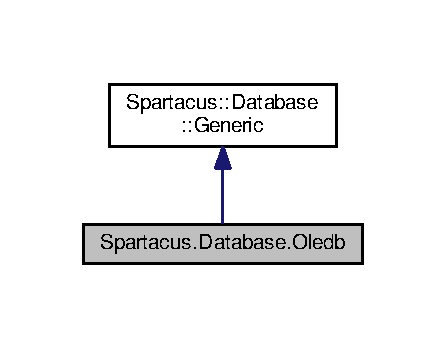
\includegraphics[width=214pt]{classSpartacus_1_1Database_1_1Oledb__inherit__graph}
\end{center}
\end{figure}


Diagrama de colaboração para Spartacus.\+Database.\+Oledb\+:\nopagebreak
\begin{figure}[H]
\begin{center}
\leavevmode
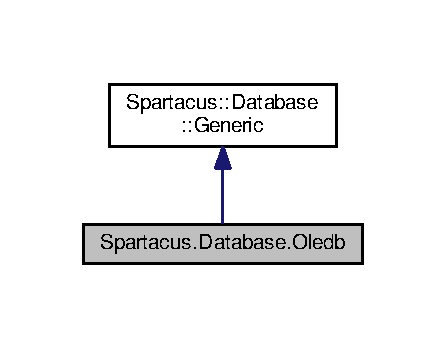
\includegraphics[width=214pt]{classSpartacus_1_1Database_1_1Oledb__coll__graph}
\end{center}
\end{figure}
\subsection*{Métodos Públicos}
\begin{DoxyCompactItemize}
\item 
\hyperlink{classSpartacus_1_1Database_1_1Oledb_a151e92500d1aa88e96169201d3138b0a}{Oledb} (string p\+\_\+provider, string p\+\_\+host, string p\+\_\+port, string p\+\_\+service, string p\+\_\+user, string p\+\_\+password)
\begin{DoxyCompactList}\small\item\em Inicializa uma nova instância da classe \hyperlink{classSpartacus_1_1Database_1_1Oledb}{Spartacus.\+Database.\+Oledb}. Cria a string de conexão ao banco. \end{DoxyCompactList}\item 
override System.\+Data.\+Data\+Table \hyperlink{classSpartacus_1_1Database_1_1Oledb_a6f914652553778f6e0a683ac92ab1f87}{Query} (string p\+\_\+sql, string p\+\_\+tablename)
\begin{DoxyCompactList}\small\item\em Realiza uma consulta no banco de dados, armazenando os dados de retorno em um System.\+Data.\+Data\+Table. \end{DoxyCompactList}\item 
override System.\+Data.\+Data\+Table \hyperlink{classSpartacus_1_1Database_1_1Oledb_ab5f3ae20ac53dcc95182c0845a04d460}{Query} (string p\+\_\+sql, string p\+\_\+tablename, System.\+Data.\+Data\+Table p\+\_\+table)
\begin{DoxyCompactList}\small\item\em Realiza uma consulta no banco de dados, armazenando os dados de retorno em um System.\+Data.\+Data\+Table. \end{DoxyCompactList}\item 
override void \hyperlink{classSpartacus_1_1Database_1_1Oledb_acfe60cb51ca949f93a1197c3cdf88231}{Execute} (string p\+\_\+sql)
\begin{DoxyCompactList}\small\item\em Executa um código S\+Q\+L no banco de dados. \end{DoxyCompactList}\item 
override string \hyperlink{classSpartacus_1_1Database_1_1Oledb_a7131081aa9dcb742321104b3a2c0c1f5}{Execute\+Scalar} (string p\+\_\+sql)
\begin{DoxyCompactList}\small\item\em Realiza uma consulta no banco de dados, armazenando um único dado de retorno em uma string. \end{DoxyCompactList}\end{DoxyCompactItemize}
\subsection*{Campos de Dados}
\begin{DoxyCompactItemize}
\item 
string \hyperlink{classSpartacus_1_1Database_1_1Oledb_a7bfa2fa4427cb9a5ae00fc0e58562ece}{v\+\_\+connectionstring}
\begin{DoxyCompactList}\small\item\em String de conexão para acessar o banco. \end{DoxyCompactList}\end{DoxyCompactItemize}


\subsection{Descrição Detalhada}
Classe \hyperlink{classSpartacus_1_1Database_1_1Oledb}{Spartacus.\+Database.\+Oledb}; Herda da classe \hyperlink{classSpartacus_1_1Database_1_1Generic}{Spartacus.\+Database.\+Generic}. Utiliza a implementação O\+L\+E D\+B para acessar qualquer S\+G\+B\+D. 



\subsection{Construtores \& Destrutores}
\hypertarget{classSpartacus_1_1Database_1_1Oledb_a151e92500d1aa88e96169201d3138b0a}{\index{Spartacus\+::\+Database\+::\+Oledb@{Spartacus\+::\+Database\+::\+Oledb}!Oledb@{Oledb}}
\index{Oledb@{Oledb}!Spartacus\+::\+Database\+::\+Oledb@{Spartacus\+::\+Database\+::\+Oledb}}
\subsubsection[{Oledb}]{\setlength{\rightskip}{0pt plus 5cm}Spartacus.\+Database.\+Oledb.\+Oledb (
\begin{DoxyParamCaption}
\item[{string}]{p\+\_\+provider, }
\item[{string}]{p\+\_\+host, }
\item[{string}]{p\+\_\+port, }
\item[{string}]{p\+\_\+service, }
\item[{string}]{p\+\_\+user, }
\item[{string}]{p\+\_\+password}
\end{DoxyParamCaption}
)\hspace{0.3cm}{\ttfamily [inline]}}}\label{classSpartacus_1_1Database_1_1Oledb_a151e92500d1aa88e96169201d3138b0a}


Inicializa uma nova instância da classe \hyperlink{classSpartacus_1_1Database_1_1Oledb}{Spartacus.\+Database.\+Oledb}. Cria a string de conexão ao banco. 


\begin{DoxyParams}{Parâmetros}
{\em p\+\_\+provider} & S\+G\+B\+D que fornece o banco de dados. \\
\hline
{\em p\+\_\+host} & Hostname ou I\+P onde o banco de dados está localizado. \\
\hline
{\em p\+\_\+port} & Porta T\+C\+P para conectar-\/se ao S\+G\+B\+G. \\
\hline
{\em p\+\_\+service} & Nome do serviço que representa o banco ao qual desejamos nos conectar. \\
\hline
{\em p\+\_\+user} & Usuário ou schema para se conectar ao banco de dados. \\
\hline
{\em p\+\_\+password} & A senha do usuário ou schema. \\
\hline
\end{DoxyParams}


\subsection{Métodos}
\hypertarget{classSpartacus_1_1Database_1_1Oledb_acfe60cb51ca949f93a1197c3cdf88231}{\index{Spartacus\+::\+Database\+::\+Oledb@{Spartacus\+::\+Database\+::\+Oledb}!Execute@{Execute}}
\index{Execute@{Execute}!Spartacus\+::\+Database\+::\+Oledb@{Spartacus\+::\+Database\+::\+Oledb}}
\subsubsection[{Execute}]{\setlength{\rightskip}{0pt plus 5cm}override void Spartacus.\+Database.\+Oledb.\+Execute (
\begin{DoxyParamCaption}
\item[{string}]{p\+\_\+sql}
\end{DoxyParamCaption}
)\hspace{0.3cm}{\ttfamily [inline]}, {\ttfamily [virtual]}}}\label{classSpartacus_1_1Database_1_1Oledb_acfe60cb51ca949f93a1197c3cdf88231}


Executa um código S\+Q\+L no banco de dados. 


\begin{DoxyParams}{Parâmetros}
{\em p\+\_\+sql} & Código S\+Q\+L a ser executado no banco de dados. \\
\hline
\end{DoxyParams}

\begin{DoxyExceptions}{Exceções}
{\em \hyperlink{classSpartacus_1_1Database_1_1Exception}{Spartacus.\+Database.\+Exception}} & Exceção acontece quando não for possível executar o código S\+Q\+L.\\
\hline
\end{DoxyExceptions}


Implementa \hyperlink{classSpartacus_1_1Database_1_1Generic_a28f1c8821906653eb4ff1484de893d16}{Spartacus.\+Database.\+Generic}.

\hypertarget{classSpartacus_1_1Database_1_1Oledb_a7131081aa9dcb742321104b3a2c0c1f5}{\index{Spartacus\+::\+Database\+::\+Oledb@{Spartacus\+::\+Database\+::\+Oledb}!Execute\+Scalar@{Execute\+Scalar}}
\index{Execute\+Scalar@{Execute\+Scalar}!Spartacus\+::\+Database\+::\+Oledb@{Spartacus\+::\+Database\+::\+Oledb}}
\subsubsection[{Execute\+Scalar}]{\setlength{\rightskip}{0pt plus 5cm}override string Spartacus.\+Database.\+Oledb.\+Execute\+Scalar (
\begin{DoxyParamCaption}
\item[{string}]{p\+\_\+sql}
\end{DoxyParamCaption}
)\hspace{0.3cm}{\ttfamily [inline]}, {\ttfamily [virtual]}}}\label{classSpartacus_1_1Database_1_1Oledb_a7131081aa9dcb742321104b3a2c0c1f5}


Realiza uma consulta no banco de dados, armazenando um único dado de retorno em uma string. 

\begin{DoxyReturn}{Retorna}
string com o dado de retorno. 
\end{DoxyReturn}

\begin{DoxyParams}{Parâmetros}
{\em p\+\_\+sql} & Código S\+Q\+L a ser consultado no banco de dados. \\
\hline
\end{DoxyParams}

\begin{DoxyExceptions}{Exceções}
{\em \hyperlink{classSpartacus_1_1Database_1_1Exception}{Spartacus.\+Database.\+Exception}} & Exceção acontece quando não for possível executar o código S\+Q\+L.\\
\hline
\end{DoxyExceptions}


Implementa \hyperlink{classSpartacus_1_1Database_1_1Generic_a983620fd71f520deb71ae55304b98bf6}{Spartacus.\+Database.\+Generic}.

\hypertarget{classSpartacus_1_1Database_1_1Oledb_a6f914652553778f6e0a683ac92ab1f87}{\index{Spartacus\+::\+Database\+::\+Oledb@{Spartacus\+::\+Database\+::\+Oledb}!Query@{Query}}
\index{Query@{Query}!Spartacus\+::\+Database\+::\+Oledb@{Spartacus\+::\+Database\+::\+Oledb}}
\subsubsection[{Query}]{\setlength{\rightskip}{0pt plus 5cm}override System.\+Data.\+Data\+Table Spartacus.\+Database.\+Oledb.\+Query (
\begin{DoxyParamCaption}
\item[{string}]{p\+\_\+sql, }
\item[{string}]{p\+\_\+tablename}
\end{DoxyParamCaption}
)\hspace{0.3cm}{\ttfamily [inline]}, {\ttfamily [virtual]}}}\label{classSpartacus_1_1Database_1_1Oledb_a6f914652553778f6e0a683ac92ab1f87}


Realiza uma consulta no banco de dados, armazenando os dados de retorno em um System.\+Data.\+Data\+Table. 


\begin{DoxyParams}{Parâmetros}
{\em p\+\_\+sql} & Código S\+Q\+L a ser consultado no banco de dados. \\
\hline
{\em p\+\_\+tablename} & Nome virtual da tabela onde deve ser armazenado o resultado, para fins de cache. \\
\hline
\end{DoxyParams}
\begin{DoxyReturn}{Retorna}
Retorna uma System.\+Data.\+Data\+Table com os dados de retorno da consulta.
\end{DoxyReturn}

\begin{DoxyExceptions}{Exceções}
{\em \hyperlink{classSpartacus_1_1Database_1_1Exception}{Spartacus.\+Database.\+Exception}} & Exceção acontece quando não for possível executar a consulta.\\
\hline
\end{DoxyExceptions}


Implementa \hyperlink{classSpartacus_1_1Database_1_1Generic_a23dc0eb8f4722d1adb1935044bc878ff}{Spartacus.\+Database.\+Generic}.

\hypertarget{classSpartacus_1_1Database_1_1Oledb_ab5f3ae20ac53dcc95182c0845a04d460}{\index{Spartacus\+::\+Database\+::\+Oledb@{Spartacus\+::\+Database\+::\+Oledb}!Query@{Query}}
\index{Query@{Query}!Spartacus\+::\+Database\+::\+Oledb@{Spartacus\+::\+Database\+::\+Oledb}}
\subsubsection[{Query}]{\setlength{\rightskip}{0pt plus 5cm}override System.\+Data.\+Data\+Table Spartacus.\+Database.\+Oledb.\+Query (
\begin{DoxyParamCaption}
\item[{string}]{p\+\_\+sql, }
\item[{string}]{p\+\_\+tablename, }
\item[{System.\+Data.\+Data\+Table}]{p\+\_\+table}
\end{DoxyParamCaption}
)\hspace{0.3cm}{\ttfamily [inline]}, {\ttfamily [virtual]}}}\label{classSpartacus_1_1Database_1_1Oledb_ab5f3ae20ac53dcc95182c0845a04d460}


Realiza uma consulta no banco de dados, armazenando os dados de retorno em um System.\+Data.\+Data\+Table. 


\begin{DoxyParams}{Parâmetros}
{\em p\+\_\+sql} & Código S\+Q\+L a ser consultado no banco de dados. \\
\hline
{\em p\+\_\+tablename} & Nome virtual da tabela onde deve ser armazenado o resultado, para fins de cache. \\
\hline
{\em p\+\_\+table} & Tabela que contém definições de nomes e tipos de colunas. \\
\hline
\end{DoxyParams}
\begin{DoxyReturn}{Retorna}
Retorna uma System.\+Data.\+Data\+Table com os dados de retorno da consulta.
\end{DoxyReturn}

\begin{DoxyExceptions}{Exceções}
{\em \hyperlink{classSpartacus_1_1Database_1_1Exception}{Spartacus.\+Database.\+Exception}} & Exceção acontece quando não for possível executar a consulta.\\
\hline
\end{DoxyExceptions}


Implementa \hyperlink{classSpartacus_1_1Database_1_1Generic_a434ce0b27dfa73d909bc79c0b8471e54}{Spartacus.\+Database.\+Generic}.



\subsection{Campos}
\hypertarget{classSpartacus_1_1Database_1_1Oledb_a7bfa2fa4427cb9a5ae00fc0e58562ece}{\index{Spartacus\+::\+Database\+::\+Oledb@{Spartacus\+::\+Database\+::\+Oledb}!v\+\_\+connectionstring@{v\+\_\+connectionstring}}
\index{v\+\_\+connectionstring@{v\+\_\+connectionstring}!Spartacus\+::\+Database\+::\+Oledb@{Spartacus\+::\+Database\+::\+Oledb}}
\subsubsection[{v\+\_\+connectionstring}]{\setlength{\rightskip}{0pt plus 5cm}string Spartacus.\+Database.\+Oledb.\+v\+\_\+connectionstring}}\label{classSpartacus_1_1Database_1_1Oledb_a7bfa2fa4427cb9a5ae00fc0e58562ece}


String de conexão para acessar o banco. 



A documentação para esta classe foi gerada a partir do seguinte arquivo\+:\begin{DoxyCompactItemize}
\item 
Spartacus.\+Database.\+Oledb.\+cs\end{DoxyCompactItemize}

\hypertarget{classSpartacus_1_1Database_1_1Parameter}{\section{Referência da Classe Spartacus.\+Database.\+Parameter}
\label{classSpartacus_1_1Database_1_1Parameter}\index{Spartacus.\+Database.\+Parameter@{Spartacus.\+Database.\+Parameter}}
}


Classe \hyperlink{classSpartacus_1_1Database_1_1Parameter}{Parameter}. Representa um parâmetro da classe \hyperlink{classSpartacus_1_1Database_1_1Command}{Spartacus.\+Database.\+Command}.  


\subsection*{Métodos Públicos}
\begin{DoxyCompactItemize}
\item 
\hyperlink{classSpartacus_1_1Database_1_1Parameter_abb88975fcb3c617dfd1507876423d0f8}{Parameter} (String p\+\_\+name, \hyperlink{namespaceSpartacus_1_1Database_a9d4c2be7c9bc257b8d34c84b43e5ec32}{Spartacus.\+Database.\+Type} p\+\_\+type)
\begin{DoxyCompactList}\small\item\em Inicializa uma instância da classe \hyperlink{classSpartacus_1_1Database_1_1Parameter}{Spartacus.\+Database.\+Parameter} . \end{DoxyCompactList}\item 
string \hyperlink{classSpartacus_1_1Database_1_1Parameter_a2402087cb5b054351038a72541e0bdf8}{Text} ()
\begin{DoxyCompactList}\small\item\em Escreve o valor do Parâmetro em formato de string, para ser usado dentro do Comando S\+Q\+L. Monta a string de acordo com os atributos do Parâmetro. \end{DoxyCompactList}\end{DoxyCompactItemize}
\subsection*{Campos de Dados}
\begin{DoxyCompactItemize}
\item 
string \hyperlink{classSpartacus_1_1Database_1_1Parameter_a5bea1044f316cf4507de807026b1599a}{v\+\_\+name}
\begin{DoxyCompactList}\small\item\em Nome do Parâmetro dentro do Comando S\+Q\+L. Deve ser único dentro de uma mesma classe \hyperlink{classSpartacus_1_1Database_1_1Command}{Spartacus.\+Database.\+Command}. \end{DoxyCompactList}\item 
\hyperlink{namespaceSpartacus_1_1Database_a9d4c2be7c9bc257b8d34c84b43e5ec32}{Spartacus.\+Database.\+Type} \hyperlink{classSpartacus_1_1Database_1_1Parameter_a0185e9a5eb61471aed6a5fe31f7fdac6}{v\+\_\+type}
\begin{DoxyCompactList}\small\item\em Tipo de Dados. \end{DoxyCompactList}\item 
string \hyperlink{classSpartacus_1_1Database_1_1Parameter_a124939a3bf560bd654e83b54f94c522b}{v\+\_\+value}
\begin{DoxyCompactList}\small\item\em Valor atual do Parâmetro. \end{DoxyCompactList}\item 
string \hyperlink{classSpartacus_1_1Database_1_1Parameter_a55aba864768ac148a7153eb51b7cf845}{v\+\_\+dateformat}
\begin{DoxyCompactList}\small\item\em Formato de Data, usado se caso o Parâmetro for do tipo D\+A\+T\+E. \end{DoxyCompactList}\item 
\hyperlink{namespaceSpartacus_1_1Database_a5c77dce887cad55e7ea67f0f98a7d71f}{Spartacus.\+Database.\+Locale} \hyperlink{classSpartacus_1_1Database_1_1Parameter_abc543efca34bb719b603e7157202b37a}{v\+\_\+locale}
\begin{DoxyCompactList}\small\item\em Localização, representação de números reais. \end{DoxyCompactList}\item 
bool \hyperlink{classSpartacus_1_1Database_1_1Parameter_af422ee9e94e89ad0994b6ac2de2833ba}{v\+\_\+null}
\begin{DoxyCompactList}\small\item\em Indica se o Parâmetro possui valor N\+U\+L\+L ou não. \end{DoxyCompactList}\item 
string \hyperlink{classSpartacus_1_1Database_1_1Parameter_a94ea1be55d0301fa86f274a52206c214}{v\+\_\+description}
\begin{DoxyCompactList}\small\item\em Descrição do parâmetro, a ser mostrado para o usuário. \end{DoxyCompactList}\end{DoxyCompactItemize}


\subsection{Descrição Detalhada}
Classe \hyperlink{classSpartacus_1_1Database_1_1Parameter}{Parameter}. Representa um parâmetro da classe \hyperlink{classSpartacus_1_1Database_1_1Command}{Spartacus.\+Database.\+Command}. 



\subsection{Construtores \& Destrutores}
\hypertarget{classSpartacus_1_1Database_1_1Parameter_abb88975fcb3c617dfd1507876423d0f8}{\index{Spartacus\+::\+Database\+::\+Parameter@{Spartacus\+::\+Database\+::\+Parameter}!Parameter@{Parameter}}
\index{Parameter@{Parameter}!Spartacus\+::\+Database\+::\+Parameter@{Spartacus\+::\+Database\+::\+Parameter}}
\subsubsection[{Parameter}]{\setlength{\rightskip}{0pt plus 5cm}Spartacus.\+Database.\+Parameter.\+Parameter (
\begin{DoxyParamCaption}
\item[{String}]{p\+\_\+name, }
\item[{{\bf Spartacus.\+Database.\+Type}}]{p\+\_\+type}
\end{DoxyParamCaption}
)\hspace{0.3cm}{\ttfamily [inline]}}}\label{classSpartacus_1_1Database_1_1Parameter_abb88975fcb3c617dfd1507876423d0f8}


Inicializa uma instância da classe \hyperlink{classSpartacus_1_1Database_1_1Parameter}{Spartacus.\+Database.\+Parameter} . 


\begin{DoxyParams}{Parâmetros}
{\em p\+\_\+name} & Nome do parâmetro dentro do Comando S\+Q\+L. \\
\hline
{\em p\+\_\+type} & Tipo de dados do parâmetro. \\
\hline
\end{DoxyParams}


\subsection{Métodos}
\hypertarget{classSpartacus_1_1Database_1_1Parameter_a2402087cb5b054351038a72541e0bdf8}{\index{Spartacus\+::\+Database\+::\+Parameter@{Spartacus\+::\+Database\+::\+Parameter}!Text@{Text}}
\index{Text@{Text}!Spartacus\+::\+Database\+::\+Parameter@{Spartacus\+::\+Database\+::\+Parameter}}
\subsubsection[{Text}]{\setlength{\rightskip}{0pt plus 5cm}string Spartacus.\+Database.\+Parameter.\+Text (
\begin{DoxyParamCaption}
{}
\end{DoxyParamCaption}
)\hspace{0.3cm}{\ttfamily [inline]}}}\label{classSpartacus_1_1Database_1_1Parameter_a2402087cb5b054351038a72541e0bdf8}


Escreve o valor do Parâmetro em formato de string, para ser usado dentro do Comando S\+Q\+L. Monta a string de acordo com os atributos do Parâmetro. 



\subsection{Campos}
\hypertarget{classSpartacus_1_1Database_1_1Parameter_a55aba864768ac148a7153eb51b7cf845}{\index{Spartacus\+::\+Database\+::\+Parameter@{Spartacus\+::\+Database\+::\+Parameter}!v\+\_\+dateformat@{v\+\_\+dateformat}}
\index{v\+\_\+dateformat@{v\+\_\+dateformat}!Spartacus\+::\+Database\+::\+Parameter@{Spartacus\+::\+Database\+::\+Parameter}}
\subsubsection[{v\+\_\+dateformat}]{\setlength{\rightskip}{0pt plus 5cm}string Spartacus.\+Database.\+Parameter.\+v\+\_\+dateformat}}\label{classSpartacus_1_1Database_1_1Parameter_a55aba864768ac148a7153eb51b7cf845}


Formato de Data, usado se caso o Parâmetro for do tipo D\+A\+T\+E. 

\hypertarget{classSpartacus_1_1Database_1_1Parameter_a94ea1be55d0301fa86f274a52206c214}{\index{Spartacus\+::\+Database\+::\+Parameter@{Spartacus\+::\+Database\+::\+Parameter}!v\+\_\+description@{v\+\_\+description}}
\index{v\+\_\+description@{v\+\_\+description}!Spartacus\+::\+Database\+::\+Parameter@{Spartacus\+::\+Database\+::\+Parameter}}
\subsubsection[{v\+\_\+description}]{\setlength{\rightskip}{0pt plus 5cm}string Spartacus.\+Database.\+Parameter.\+v\+\_\+description}}\label{classSpartacus_1_1Database_1_1Parameter_a94ea1be55d0301fa86f274a52206c214}


Descrição do parâmetro, a ser mostrado para o usuário. 

\hypertarget{classSpartacus_1_1Database_1_1Parameter_abc543efca34bb719b603e7157202b37a}{\index{Spartacus\+::\+Database\+::\+Parameter@{Spartacus\+::\+Database\+::\+Parameter}!v\+\_\+locale@{v\+\_\+locale}}
\index{v\+\_\+locale@{v\+\_\+locale}!Spartacus\+::\+Database\+::\+Parameter@{Spartacus\+::\+Database\+::\+Parameter}}
\subsubsection[{v\+\_\+locale}]{\setlength{\rightskip}{0pt plus 5cm}{\bf Spartacus.\+Database.\+Locale} Spartacus.\+Database.\+Parameter.\+v\+\_\+locale}}\label{classSpartacus_1_1Database_1_1Parameter_abc543efca34bb719b603e7157202b37a}


Localização, representação de números reais. 

\hypertarget{classSpartacus_1_1Database_1_1Parameter_a5bea1044f316cf4507de807026b1599a}{\index{Spartacus\+::\+Database\+::\+Parameter@{Spartacus\+::\+Database\+::\+Parameter}!v\+\_\+name@{v\+\_\+name}}
\index{v\+\_\+name@{v\+\_\+name}!Spartacus\+::\+Database\+::\+Parameter@{Spartacus\+::\+Database\+::\+Parameter}}
\subsubsection[{v\+\_\+name}]{\setlength{\rightskip}{0pt plus 5cm}string Spartacus.\+Database.\+Parameter.\+v\+\_\+name}}\label{classSpartacus_1_1Database_1_1Parameter_a5bea1044f316cf4507de807026b1599a}


Nome do Parâmetro dentro do Comando S\+Q\+L. Deve ser único dentro de uma mesma classe \hyperlink{classSpartacus_1_1Database_1_1Command}{Spartacus.\+Database.\+Command}. 

\hypertarget{classSpartacus_1_1Database_1_1Parameter_af422ee9e94e89ad0994b6ac2de2833ba}{\index{Spartacus\+::\+Database\+::\+Parameter@{Spartacus\+::\+Database\+::\+Parameter}!v\+\_\+null@{v\+\_\+null}}
\index{v\+\_\+null@{v\+\_\+null}!Spartacus\+::\+Database\+::\+Parameter@{Spartacus\+::\+Database\+::\+Parameter}}
\subsubsection[{v\+\_\+null}]{\setlength{\rightskip}{0pt plus 5cm}bool Spartacus.\+Database.\+Parameter.\+v\+\_\+null}}\label{classSpartacus_1_1Database_1_1Parameter_af422ee9e94e89ad0994b6ac2de2833ba}


Indica se o Parâmetro possui valor N\+U\+L\+L ou não. 

\hypertarget{classSpartacus_1_1Database_1_1Parameter_a0185e9a5eb61471aed6a5fe31f7fdac6}{\index{Spartacus\+::\+Database\+::\+Parameter@{Spartacus\+::\+Database\+::\+Parameter}!v\+\_\+type@{v\+\_\+type}}
\index{v\+\_\+type@{v\+\_\+type}!Spartacus\+::\+Database\+::\+Parameter@{Spartacus\+::\+Database\+::\+Parameter}}
\subsubsection[{v\+\_\+type}]{\setlength{\rightskip}{0pt plus 5cm}{\bf Spartacus.\+Database.\+Type} Spartacus.\+Database.\+Parameter.\+v\+\_\+type}}\label{classSpartacus_1_1Database_1_1Parameter_a0185e9a5eb61471aed6a5fe31f7fdac6}


Tipo de Dados. 

\hypertarget{classSpartacus_1_1Database_1_1Parameter_a124939a3bf560bd654e83b54f94c522b}{\index{Spartacus\+::\+Database\+::\+Parameter@{Spartacus\+::\+Database\+::\+Parameter}!v\+\_\+value@{v\+\_\+value}}
\index{v\+\_\+value@{v\+\_\+value}!Spartacus\+::\+Database\+::\+Parameter@{Spartacus\+::\+Database\+::\+Parameter}}
\subsubsection[{v\+\_\+value}]{\setlength{\rightskip}{0pt plus 5cm}string Spartacus.\+Database.\+Parameter.\+v\+\_\+value}}\label{classSpartacus_1_1Database_1_1Parameter_a124939a3bf560bd654e83b54f94c522b}


Valor atual do Parâmetro. 



A documentação para esta classe foi gerada a partir do seguinte arquivo\+:\begin{DoxyCompactItemize}
\item 
Spartacus.\+Database.\+Parameter.\+cs\end{DoxyCompactItemize}

\hypertarget{classSpartacus_1_1Database_1_1Sqlite}{\section{Referência da Classe Spartacus.\+Database.\+Sqlite}
\label{classSpartacus_1_1Database_1_1Sqlite}\index{Spartacus.\+Database.\+Sqlite@{Spartacus.\+Database.\+Sqlite}}
}


Classe \hyperlink{classSpartacus_1_1Database_1_1Sqlite}{Spartacus.\+Database.\+Sqlite}. Herda da classe \hyperlink{classSpartacus_1_1Database_1_1Generic}{Spartacus.\+Database.\+Generic}. Utiliza o Mono.\+Data.\+Sqlite para acessar um S\+G\+B\+D \hyperlink{classSpartacus_1_1Database_1_1Sqlite}{Sqlite}.  




Diagrama de Hierarquia para Spartacus.\+Database.\+Sqlite\+:


Diagrama de colaboração para Spartacus.\+Database.\+Sqlite\+:
\subsection*{Métodos Públicos}
\begin{DoxyCompactItemize}
\item 
\hyperlink{classSpartacus_1_1Database_1_1Sqlite_ac093bc658547c155306908a97e7e725d}{Sqlite} (string p\+\_\+file)
\begin{DoxyCompactList}\small\item\em Inicializa uma nova instancia da classe \hyperlink{classSpartacus_1_1Database_1_1Sqlite}{Spartacus.\+Database.\+Sqlite}. \end{DoxyCompactList}\item 
override void \hyperlink{classSpartacus_1_1Database_1_1Sqlite_a7bbbff1d7f1b76d0545cc6fd7ce03c32}{Connect} ()
\begin{DoxyCompactList}\small\item\em Conectar ao banco de dados. \end{DoxyCompactList}\item 
override void \hyperlink{classSpartacus_1_1Database_1_1Sqlite_a1ecb802399c8b374d23edaf4237ce667}{Disconnect} ()
\begin{DoxyCompactList}\small\item\em Desconectar do banco de dados. \end{DoxyCompactList}\item 
override System.\+Data.\+Data\+Table \hyperlink{classSpartacus_1_1Database_1_1Sqlite_a6b452dd40baf4fb82f3cf1dc2b5adef2}{Query} (string p\+\_\+sql, string p\+\_\+tablename)
\begin{DoxyCompactList}\small\item\em Realiza uma consulta no banco de dados, armazenando os dados de retorno em um System.\+Data.\+Data\+Table. \end{DoxyCompactList}\item 
override System.\+Data.\+Data\+Table \hyperlink{classSpartacus_1_1Database_1_1Sqlite_a935c96905011800e4df8ad0a7ca9bcf3}{Query} (string p\+\_\+sql, string p\+\_\+tablename, System.\+Data.\+Data\+Table p\+\_\+table)
\begin{DoxyCompactList}\small\item\em Realiza uma consulta no banco de dados, armazenando os dados de retorno em um System.\+Data.\+Data\+Table. \end{DoxyCompactList}\item 
override void \hyperlink{classSpartacus_1_1Database_1_1Sqlite_adb68d4ddb00d814f9741ec87e88d788a}{Execute} (string p\+\_\+sql)
\begin{DoxyCompactList}\small\item\em Executa um código S\+Q\+L no banco de dados. \end{DoxyCompactList}\item 
override string \hyperlink{classSpartacus_1_1Database_1_1Sqlite_a0f8931cb84b7c91dce7bd45089896d46}{Execute\+Scalar} (string p\+\_\+sql)
\begin{DoxyCompactList}\small\item\em Realiza uma consulta no banco de dados, armazenando um único dado de retorno em uma string. \end{DoxyCompactList}\end{DoxyCompactItemize}
\subsection*{Campos de Dados}
\begin{DoxyCompactItemize}
\item 
string \hyperlink{classSpartacus_1_1Database_1_1Sqlite_aef2f3f04e82b23a55a684c532f6aee99}{v\+\_\+connectionstring}
\begin{DoxyCompactList}\small\item\em String de conexão para acessar o banco. \end{DoxyCompactList}\end{DoxyCompactItemize}


\subsection{Descrição Detalhada}
Classe \hyperlink{classSpartacus_1_1Database_1_1Sqlite}{Spartacus.\+Database.\+Sqlite}. Herda da classe \hyperlink{classSpartacus_1_1Database_1_1Generic}{Spartacus.\+Database.\+Generic}. Utiliza o Mono.\+Data.\+Sqlite para acessar um S\+G\+B\+D \hyperlink{classSpartacus_1_1Database_1_1Sqlite}{Sqlite}. 



\subsection{Construtores \& Destrutores}
\hypertarget{classSpartacus_1_1Database_1_1Sqlite_ac093bc658547c155306908a97e7e725d}{\index{Spartacus\+::\+Database\+::\+Sqlite@{Spartacus\+::\+Database\+::\+Sqlite}!Sqlite@{Sqlite}}
\index{Sqlite@{Sqlite}!Spartacus\+::\+Database\+::\+Sqlite@{Spartacus\+::\+Database\+::\+Sqlite}}
\subsubsection[{Sqlite}]{\setlength{\rightskip}{0pt plus 5cm}Spartacus.\+Database.\+Sqlite.\+Sqlite (
\begin{DoxyParamCaption}
\item[{string}]{p\+\_\+file}
\end{DoxyParamCaption}
)\hspace{0.3cm}{\ttfamily [inline]}}}\label{classSpartacus_1_1Database_1_1Sqlite_ac093bc658547c155306908a97e7e725d}


Inicializa uma nova instancia da classe \hyperlink{classSpartacus_1_1Database_1_1Sqlite}{Spartacus.\+Database.\+Sqlite}. 


\begin{DoxyParams}{Parâmetros}
{\em p\+\_\+file} & Caminho para o arquivo D\+B. \\
\hline
\end{DoxyParams}


\subsection{Métodos}
\hypertarget{classSpartacus_1_1Database_1_1Sqlite_a7bbbff1d7f1b76d0545cc6fd7ce03c32}{\index{Spartacus\+::\+Database\+::\+Sqlite@{Spartacus\+::\+Database\+::\+Sqlite}!Connect@{Connect}}
\index{Connect@{Connect}!Spartacus\+::\+Database\+::\+Sqlite@{Spartacus\+::\+Database\+::\+Sqlite}}
\subsubsection[{Connect}]{\setlength{\rightskip}{0pt plus 5cm}override void Spartacus.\+Database.\+Sqlite.\+Connect (
\begin{DoxyParamCaption}
{}
\end{DoxyParamCaption}
)\hspace{0.3cm}{\ttfamily [inline]}, {\ttfamily [virtual]}}}\label{classSpartacus_1_1Database_1_1Sqlite_a7bbbff1d7f1b76d0545cc6fd7ce03c32}


Conectar ao banco de dados. 


\begin{DoxyExceptions}{Exceções}
{\em \hyperlink{classSpartacus_1_1Database_1_1Exception}{Spartacus.\+Database.\+Exception}} & Exceção acontece quando não for possível se conectar ao banco de dados.\\
\hline
\end{DoxyExceptions}


Implementa \hyperlink{classSpartacus_1_1Database_1_1Generic_a0f3940aeabde41676f15366e83eff166}{Spartacus.\+Database.\+Generic}.

\hypertarget{classSpartacus_1_1Database_1_1Sqlite_a1ecb802399c8b374d23edaf4237ce667}{\index{Spartacus\+::\+Database\+::\+Sqlite@{Spartacus\+::\+Database\+::\+Sqlite}!Disconnect@{Disconnect}}
\index{Disconnect@{Disconnect}!Spartacus\+::\+Database\+::\+Sqlite@{Spartacus\+::\+Database\+::\+Sqlite}}
\subsubsection[{Disconnect}]{\setlength{\rightskip}{0pt plus 5cm}override void Spartacus.\+Database.\+Sqlite.\+Disconnect (
\begin{DoxyParamCaption}
{}
\end{DoxyParamCaption}
)\hspace{0.3cm}{\ttfamily [inline]}, {\ttfamily [virtual]}}}\label{classSpartacus_1_1Database_1_1Sqlite_a1ecb802399c8b374d23edaf4237ce667}


Desconectar do banco de dados. 


\begin{DoxyExceptions}{Exceções}
{\em \hyperlink{classSpartacus_1_1Database_1_1Exception}{Spartacus.\+Database.\+Exception}} & Exceção acontece quando não for possível se desconectar do banco de dados.\\
\hline
\end{DoxyExceptions}


Implementa \hyperlink{classSpartacus_1_1Database_1_1Generic_a765dda5d5d8a768885fabd9799a0a180}{Spartacus.\+Database.\+Generic}.

\hypertarget{classSpartacus_1_1Database_1_1Sqlite_adb68d4ddb00d814f9741ec87e88d788a}{\index{Spartacus\+::\+Database\+::\+Sqlite@{Spartacus\+::\+Database\+::\+Sqlite}!Execute@{Execute}}
\index{Execute@{Execute}!Spartacus\+::\+Database\+::\+Sqlite@{Spartacus\+::\+Database\+::\+Sqlite}}
\subsubsection[{Execute}]{\setlength{\rightskip}{0pt plus 5cm}override void Spartacus.\+Database.\+Sqlite.\+Execute (
\begin{DoxyParamCaption}
\item[{string}]{p\+\_\+sql}
\end{DoxyParamCaption}
)\hspace{0.3cm}{\ttfamily [inline]}, {\ttfamily [virtual]}}}\label{classSpartacus_1_1Database_1_1Sqlite_adb68d4ddb00d814f9741ec87e88d788a}


Executa um código S\+Q\+L no banco de dados. 


\begin{DoxyParams}{Parâmetros}
{\em p\+\_\+sql} & Código S\+Q\+L a ser executado no banco de dados. \\
\hline
\end{DoxyParams}

\begin{DoxyExceptions}{Exceções}
{\em \hyperlink{classSpartacus_1_1Database_1_1Exception}{Spartacus.\+Database.\+Exception}} & Exceção acontece quando não for possível executar o código S\+Q\+L.\\
\hline
\end{DoxyExceptions}


Implementa \hyperlink{classSpartacus_1_1Database_1_1Generic_a28f1c8821906653eb4ff1484de893d16}{Spartacus.\+Database.\+Generic}.

\hypertarget{classSpartacus_1_1Database_1_1Sqlite_a0f8931cb84b7c91dce7bd45089896d46}{\index{Spartacus\+::\+Database\+::\+Sqlite@{Spartacus\+::\+Database\+::\+Sqlite}!Execute\+Scalar@{Execute\+Scalar}}
\index{Execute\+Scalar@{Execute\+Scalar}!Spartacus\+::\+Database\+::\+Sqlite@{Spartacus\+::\+Database\+::\+Sqlite}}
\subsubsection[{Execute\+Scalar}]{\setlength{\rightskip}{0pt plus 5cm}override string Spartacus.\+Database.\+Sqlite.\+Execute\+Scalar (
\begin{DoxyParamCaption}
\item[{string}]{p\+\_\+sql}
\end{DoxyParamCaption}
)\hspace{0.3cm}{\ttfamily [inline]}, {\ttfamily [virtual]}}}\label{classSpartacus_1_1Database_1_1Sqlite_a0f8931cb84b7c91dce7bd45089896d46}


Realiza uma consulta no banco de dados, armazenando um único dado de retorno em uma string. 

\begin{DoxyReturn}{Retorna}
string com o dado de retorno. 
\end{DoxyReturn}

\begin{DoxyParams}{Parâmetros}
{\em p\+\_\+sql} & Código S\+Q\+L a ser consultado no banco de dados. \\
\hline
\end{DoxyParams}

\begin{DoxyExceptions}{Exceções}
{\em \hyperlink{classSpartacus_1_1Database_1_1Exception}{Spartacus.\+Database.\+Exception}} & Exceção acontece quando não for possível executar o código S\+Q\+L.\\
\hline
\end{DoxyExceptions}


Implementa \hyperlink{classSpartacus_1_1Database_1_1Generic_a983620fd71f520deb71ae55304b98bf6}{Spartacus.\+Database.\+Generic}.

\hypertarget{classSpartacus_1_1Database_1_1Sqlite_a6b452dd40baf4fb82f3cf1dc2b5adef2}{\index{Spartacus\+::\+Database\+::\+Sqlite@{Spartacus\+::\+Database\+::\+Sqlite}!Query@{Query}}
\index{Query@{Query}!Spartacus\+::\+Database\+::\+Sqlite@{Spartacus\+::\+Database\+::\+Sqlite}}
\subsubsection[{Query}]{\setlength{\rightskip}{0pt plus 5cm}override System.\+Data.\+Data\+Table Spartacus.\+Database.\+Sqlite.\+Query (
\begin{DoxyParamCaption}
\item[{string}]{p\+\_\+sql, }
\item[{string}]{p\+\_\+tablename}
\end{DoxyParamCaption}
)\hspace{0.3cm}{\ttfamily [inline]}, {\ttfamily [virtual]}}}\label{classSpartacus_1_1Database_1_1Sqlite_a6b452dd40baf4fb82f3cf1dc2b5adef2}


Realiza uma consulta no banco de dados, armazenando os dados de retorno em um System.\+Data.\+Data\+Table. 


\begin{DoxyParams}{Parâmetros}
{\em p\+\_\+sql} & Código S\+Q\+L a ser consultado no banco de dados. \\
\hline
{\em p\+\_\+tablename} & Nome virtual da tabela onde deve ser armazenado o resultado, para fins de cache. \\
\hline
\end{DoxyParams}
\begin{DoxyReturn}{Retorna}
Retorna uma System.\+Data.\+Data\+Table com os dados de retorno da consulta.
\end{DoxyReturn}

\begin{DoxyExceptions}{Exceções}
{\em \hyperlink{classSpartacus_1_1Database_1_1Exception}{Spartacus.\+Database.\+Exception}} & Exceção acontece quando não for possível executar a consulta.\\
\hline
\end{DoxyExceptions}


Implementa \hyperlink{classSpartacus_1_1Database_1_1Generic_a23dc0eb8f4722d1adb1935044bc878ff}{Spartacus.\+Database.\+Generic}.

\hypertarget{classSpartacus_1_1Database_1_1Sqlite_a935c96905011800e4df8ad0a7ca9bcf3}{\index{Spartacus\+::\+Database\+::\+Sqlite@{Spartacus\+::\+Database\+::\+Sqlite}!Query@{Query}}
\index{Query@{Query}!Spartacus\+::\+Database\+::\+Sqlite@{Spartacus\+::\+Database\+::\+Sqlite}}
\subsubsection[{Query}]{\setlength{\rightskip}{0pt plus 5cm}override System.\+Data.\+Data\+Table Spartacus.\+Database.\+Sqlite.\+Query (
\begin{DoxyParamCaption}
\item[{string}]{p\+\_\+sql, }
\item[{string}]{p\+\_\+tablename, }
\item[{System.\+Data.\+Data\+Table}]{p\+\_\+table}
\end{DoxyParamCaption}
)\hspace{0.3cm}{\ttfamily [inline]}, {\ttfamily [virtual]}}}\label{classSpartacus_1_1Database_1_1Sqlite_a935c96905011800e4df8ad0a7ca9bcf3}


Realiza uma consulta no banco de dados, armazenando os dados de retorno em um System.\+Data.\+Data\+Table. 


\begin{DoxyParams}{Parâmetros}
{\em p\+\_\+sql} & Código S\+Q\+L a ser consultado no banco de dados. \\
\hline
{\em p\+\_\+tablename} & Nome virtual da tabela onde deve ser armazenado o resultado, para fins de cache. \\
\hline
{\em p\+\_\+table} & Tabela que contém definições de nomes e tipos de colunas. \\
\hline
\end{DoxyParams}
\begin{DoxyReturn}{Retorna}
Retorna uma System.\+Data.\+Data\+Table com os dados de retorno da consulta.
\end{DoxyReturn}

\begin{DoxyExceptions}{Exceções}
{\em \hyperlink{classSpartacus_1_1Database_1_1Exception}{Spartacus.\+Database.\+Exception}} & Exceção acontece quando não for possível executar a consulta.\\
\hline
\end{DoxyExceptions}


Implementa \hyperlink{classSpartacus_1_1Database_1_1Generic_a434ce0b27dfa73d909bc79c0b8471e54}{Spartacus.\+Database.\+Generic}.



\subsection{Campos}
\hypertarget{classSpartacus_1_1Database_1_1Sqlite_aef2f3f04e82b23a55a684c532f6aee99}{\index{Spartacus\+::\+Database\+::\+Sqlite@{Spartacus\+::\+Database\+::\+Sqlite}!v\+\_\+connectionstring@{v\+\_\+connectionstring}}
\index{v\+\_\+connectionstring@{v\+\_\+connectionstring}!Spartacus\+::\+Database\+::\+Sqlite@{Spartacus\+::\+Database\+::\+Sqlite}}
\subsubsection[{v\+\_\+connectionstring}]{\setlength{\rightskip}{0pt plus 5cm}string Spartacus.\+Database.\+Sqlite.\+v\+\_\+connectionstring}}\label{classSpartacus_1_1Database_1_1Sqlite_aef2f3f04e82b23a55a684c532f6aee99}


String de conexão para acessar o banco. 



A documentação para esta classe foi gerada a partir do seguinte arquivo\+:\begin{DoxyCompactItemize}
\item 
Spartacus.\+Database.\+Sqlite.\+cs\end{DoxyCompactItemize}

\hypertarget{classSpartacus_1_1Utils_1_1Synchronizer}{\section{Referência da Classe Spartacus.\+Utils.\+Synchronizer}
\label{classSpartacus_1_1Utils_1_1Synchronizer}\index{Spartacus.\+Utils.\+Synchronizer@{Spartacus.\+Utils.\+Synchronizer}}
}


Classe \hyperlink{classSpartacus_1_1Utils_1_1Synchronizer}{Synchronizer}. Sincroniza duas pastas.  


\subsection*{Métodos Públicos}
\begin{DoxyCompactItemize}
\item 
\hyperlink{classSpartacus_1_1Utils_1_1Synchronizer_ab2ecf07a457f700c24ab0043d80a9079}{Synchronizer} ()
\begin{DoxyCompactList}\small\item\em Inicializa uma nova instância da classe \hyperlink{classSpartacus_1_1Utils_1_1Synchronizer}{Spartacus.\+Utils.\+Synchronizer}. \end{DoxyCompactList}\item 
void \hyperlink{classSpartacus_1_1Utils_1_1Synchronizer_a8f56ebe8182239d7b3234eec66f9da06}{Execute} (\hyperlink{namespaceSpartacus_1_1Utils_ae4b47116ae1dc35f3dc3ea735874beee}{Spartacus.\+Utils.\+Tree\+Type} p\+\_\+treetype, string p\+\_\+leftfilename, string p\+\_\+rightfilename, \hyperlink{namespaceSpartacus_1_1Utils_a835f63b39808393d4b72d203056ae42e}{Spartacus.\+Utils.\+Sync\+Action} p\+\_\+existleft\+\_\+directory\+\_\+action, \hyperlink{namespaceSpartacus_1_1Utils_a835f63b39808393d4b72d203056ae42e}{Spartacus.\+Utils.\+Sync\+Action} p\+\_\+existleft\+\_\+file\+\_\+action, \hyperlink{namespaceSpartacus_1_1Utils_a835f63b39808393d4b72d203056ae42e}{Spartacus.\+Utils.\+Sync\+Action} p\+\_\+existright\+\_\+directory\+\_\+action, \hyperlink{namespaceSpartacus_1_1Utils_a835f63b39808393d4b72d203056ae42e}{Spartacus.\+Utils.\+Sync\+Action} p\+\_\+existright\+\_\+file\+\_\+action, \hyperlink{namespaceSpartacus_1_1Utils_a835f63b39808393d4b72d203056ae42e}{Spartacus.\+Utils.\+Sync\+Action} p\+\_\+newerleft\+\_\+file\+\_\+action, \hyperlink{namespaceSpartacus_1_1Utils_a835f63b39808393d4b72d203056ae42e}{Spartacus.\+Utils.\+Sync\+Action} p\+\_\+newerright\+\_\+file\+\_\+action)
\begin{DoxyCompactList}\small\item\em Executa a comparação de diretórios e a criação de script de sincronização. \end{DoxyCompactList}\end{DoxyCompactItemize}


\subsection{Descrição Detalhada}
Classe \hyperlink{classSpartacus_1_1Utils_1_1Synchronizer}{Synchronizer}. Sincroniza duas pastas. 



\subsection{Construtores \& Destrutores}
\hypertarget{classSpartacus_1_1Utils_1_1Synchronizer_ab2ecf07a457f700c24ab0043d80a9079}{\index{Spartacus\+::\+Utils\+::\+Synchronizer@{Spartacus\+::\+Utils\+::\+Synchronizer}!Synchronizer@{Synchronizer}}
\index{Synchronizer@{Synchronizer}!Spartacus\+::\+Utils\+::\+Synchronizer@{Spartacus\+::\+Utils\+::\+Synchronizer}}
\subsubsection[{Synchronizer}]{\setlength{\rightskip}{0pt plus 5cm}Spartacus.\+Utils.\+Synchronizer.\+Synchronizer (
\begin{DoxyParamCaption}
{}
\end{DoxyParamCaption}
)\hspace{0.3cm}{\ttfamily [inline]}}}\label{classSpartacus_1_1Utils_1_1Synchronizer_ab2ecf07a457f700c24ab0043d80a9079}


Inicializa uma nova instância da classe \hyperlink{classSpartacus_1_1Utils_1_1Synchronizer}{Spartacus.\+Utils.\+Synchronizer}. 



\subsection{Métodos}
\hypertarget{classSpartacus_1_1Utils_1_1Synchronizer_a8f56ebe8182239d7b3234eec66f9da06}{\index{Spartacus\+::\+Utils\+::\+Synchronizer@{Spartacus\+::\+Utils\+::\+Synchronizer}!Execute@{Execute}}
\index{Execute@{Execute}!Spartacus\+::\+Utils\+::\+Synchronizer@{Spartacus\+::\+Utils\+::\+Synchronizer}}
\subsubsection[{Execute}]{\setlength{\rightskip}{0pt plus 5cm}void Spartacus.\+Utils.\+Synchronizer.\+Execute (
\begin{DoxyParamCaption}
\item[{{\bf Spartacus.\+Utils.\+Tree\+Type}}]{p\+\_\+treetype, }
\item[{string}]{p\+\_\+leftfilename, }
\item[{string}]{p\+\_\+rightfilename, }
\item[{{\bf Spartacus.\+Utils.\+Sync\+Action}}]{p\+\_\+existleft\+\_\+directory\+\_\+action, }
\item[{{\bf Spartacus.\+Utils.\+Sync\+Action}}]{p\+\_\+existleft\+\_\+file\+\_\+action, }
\item[{{\bf Spartacus.\+Utils.\+Sync\+Action}}]{p\+\_\+existright\+\_\+directory\+\_\+action, }
\item[{{\bf Spartacus.\+Utils.\+Sync\+Action}}]{p\+\_\+existright\+\_\+file\+\_\+action, }
\item[{{\bf Spartacus.\+Utils.\+Sync\+Action}}]{p\+\_\+newerleft\+\_\+file\+\_\+action, }
\item[{{\bf Spartacus.\+Utils.\+Sync\+Action}}]{p\+\_\+newerright\+\_\+file\+\_\+action}
\end{DoxyParamCaption}
)\hspace{0.3cm}{\ttfamily [inline]}}}\label{classSpartacus_1_1Utils_1_1Synchronizer_a8f56ebe8182239d7b3234eec66f9da06}


Executa a comparação de diretórios e a criação de script de sincronização. 


\begin{DoxyParams}{Parâmetros}
{\em p\+\_\+treetype} & Forma de obtenção da árvore de arquivos. \\
\hline
{\em p\+\_\+leftfilename} & Nome do arquivo que contém a árvore de arquivos da esquerda. \\
\hline
{\em p\+\_\+rightfilename} & Nome do arquivo que contém a árvore de arquivos da direita. \\
\hline
{\em p\+\_\+existleft\+\_\+directory\+\_\+action} & Ação a ser tomada ao ser identificado um diretório que existe apenas do lado esquerdo. \\
\hline
{\em p\+\_\+existleft\+\_\+file\+\_\+action} & Ação a ser tomada ao ser identificado um arquivo que existe apenas do lado esquerdo. \\
\hline
{\em p\+\_\+existright\+\_\+directory\+\_\+action} & Ação a ser tomada ao ser identificado um diretório que existe apenas do lado direito. \\
\hline
{\em p\+\_\+existright\+\_\+file\+\_\+action} & Ação a ser tomada ao ser identificado um arquivo que existe apenas do lado direito. \\
\hline
{\em p\+\_\+newerleft\+\_\+file\+\_\+action} & Ação a ser tomada ao ser identificado um arquivo mais recente no lado esquerdo. \\
\hline
{\em p\+\_\+newerright\+\_\+file\+\_\+action} & Ação a ser tomada ao ser identificado um arquivo mais recente no lado direito. \\
\hline
\end{DoxyParams}


A documentação para esta classe foi gerada a partir do seguinte arquivo\+:\begin{DoxyCompactItemize}
\item 
Spartacus.\+Utils.\+Synchronizer.\+cs\end{DoxyCompactItemize}

%--- End generated contents ---

% Index
\newpage
\phantomsection
\addcontentsline{toc}{chapter}{Índice}
\printindex

\end{document}
